\documentclass[a4paper,openright,12pt]{memoir}

\usepackage{color}
\providecommand{\red}[1]{\textcolor{red}{#1}}
\providecommand{\blue}[1]{\textcolor{blue}{#1}}

\usepackage{lipsum}
\nouppercaseheads
\makepagestyle{mystyle}
% \makefootrule{mystyle}{\textwidth}{\normalrulethickness}{0pt}
\makeheadrule{mystyle}{\textwidth}{\normalrulethickness}
\makeevenhead{mystyle}{Introduction to Computational Physics}{}{Gerson J. Ferreira - INFIS - UFU - Brazil}
\makeoddhead{mystyle}{}{}{\itshape\leftmark}
\makeevenfoot{mystyle}{\thepage}{}{}
\makeoddfoot{mystyle}{}{}{\thepage}
\makepsmarks{mystyle}{%
\createmark{chapter}{left}{nonumber}{}{}}
\pagestyle{mystyle}

\providecommand{\tin}{\ensuremath{<}}
\providecommand{\tout}{\ensuremath{>}}
\providecommand{\bmr}{\bm{r}} % vector r
\providecommand{\brho}{\bm{\rho}} % vector rho
\providecommand{\ket}[1]{\mbox{\ensuremath{\vert #1\rangle}}} % KET
\providecommand{\bra}[1]{\langle #1\vert} % BRA
\providecommand{\bracket}[2]{\langle #1\vert #2\rangle} % BRAKET
\providecommand{\mean}[1]{\langle #1 \rangle} % MEDIA
\providecommand{\Tr}{\ensuremath{\text{Tr}}}

\settocdepth{subsection}
\setsecnumdepth{subsection}

\usepackage[pdftex]{graphicx}
\usepackage{amssymb}
\usepackage{amsmath}
\usepackage{bm}

% \usepackage[num]{abntex2cite} % Citações padrão ABNT
\bibliographystyle{unsrt}

%  compilação de fontes
\usepackage[utf8]{inputenc}
\usepackage{fourier}
\usepackage{microtype} % para melhorias de justificação
\usepackage[dvipsnames]{xcolor} % para cores
\usepackage{graphicx} % para imagens
\usepackage{booktabs,tabularx,rotating} % para tabelas
\usepackage{mdframed} % para caixas de texto como na CIP do verso do título
\usepackage{multicol} % tabelas com colunas mescladas
\usepackage{lettrine} % letras capitulares
\usepackage{xspace} % para nao precisar de espaços com {} depois de comandos como \LaTeX e abreviações criadas pelo usuário
\usepackage{leading} % espaçamento entrelinhas (leading)
\leading{13pt}
\definecolor{blue}{RGB}{41,5,195} % alterando o aspecto da cor azul




\usepackage{minted}
\usepackage{tcolorbox}
\usepackage{etoolbox}
% \BeforeBeginEnvironment{minted}{\begin{center}\begin{tcolorbox}[width=0.95\textwidth]}%
% \AfterEndEnvironment{minted}{\end{tcolorbox}\end{center}}%
\setminted{ %
    linenos=false,            % Line numbers
    autogobble=true,          % Automatically remove common whitespace
    %bgcolor=dark-bg,
    %frame=lines,
    framesep=2mm,
    fontsize=\footnotesize
}

% ============================================================
%      ENVIRONMENT FOR EXAMPLES
% ============================================================
% ============================================================
\newcommand*\ruleline[1]{\par\noindent\raisebox{.8ex}{\makebox[\linewidth]{\hrulefill\hspace{1ex}\raisebox{-.8ex}{#1}\hspace{1ex}\hrulefill}}}
\newcounter{ctExample}
\newenvironment{example}[1]
{
    \refstepcounter{ctExample}
    \begin{center}
    \begin{tcolorbox}[width=0.95\textwidth]
    \ruleline{\texttt{Example \thectExample: #1}}
    \vspace*{-0.2cm}
}{
    \end{tcolorbox}
    \end{center}
}
\numberwithin{ctExample}{chapter}

% ============================================================
%      ENVIRONMENT FOR PROBLEMS
% ============================================================
% ============================================================
\newcounter{ctProblem}
\newenvironment{problem}[1]
{
  \refstepcounter{ctProblem}
  \noindent \textbf{Problem \thectProblem:} #1 \hrulefill
}{
  \vspace{0.3cm}
}
\numberwithin{ctProblem}{chapter}



\title{Computational Physics}
\author{Gerson J. Ferreira}
\date{\today}


% informações do PDF
\makeatletter
\usepackage{hyperref}
\hypersetup{
 %pagebackref=true,
 pageanchor=false,
 pdftitle={\@title}, 
 pdfauthor={\@author},
 pdfsubject={\@title},
 pdfcreator={LaTeX with abnTeX2},
 pdfkeywords={abnt}{latex}{abntex}{abntex2}{livro}, 
 colorlinks=true, % false: boxed links; true: colored links
 linkcolor=blue, % color of internal links
 citecolor=blue, % color of links to bibliography
 filecolor=magenta, % color of file links
 urlcolor=blue,
 bookmarksdepth=4
}
\makeatother
% ---

% Estilo de capítulos
\chapterstyle{veelo} % madsen, lyhne, pedersen, Veja outros estilos em: http://www.tex.ac.uk/tex-archive/info/MemoirChapStyles/MemoirChapStyles.pdf


% Controle do espaçamento entre um parágrafo e outro:
\setlength{\parskip}{0.2cm}  % tente também \onelineskip
%% Não recomendado mudar.

% Margens do documento 
 \setlrmarginsandblock{2.5cm}{3.5cm}{*}
 \setulmarginsandblock{2.5cm}{3.5cm}{*}
 \checkandfixthelayout
% ---





\begin{document}
\frenchspacing

\frontmatter
% \maketitle

\begin{titlingpage}
\phantom{xxx}
\vspace{0.5cm}
\huge
\raggedright
Gerson J. Ferreira \\ \normalsize Nanosciences Group \textcolor{blue}{www.infis.ufu.br/gnano}
\\
\vspace{2.5cm}
\huge 
{\raggedleft
\textit{\textcolor{blue}{Introduction to Computational Physics}}\\
\Large 
with examples in Julia \\
}
\centering
\vspace{4cm}
\huge This is a draft!\\
\Large
Please check for an updated version on\\
\url{http://www.infis.ufu.br/gerson}
\\
\large
Currently, I'm not working on this text. I'll start to review and improve/finish some sections next semester.
\vfill
\Large
Institute of Physics, Federal University of Uberlândia \\ \today
\end{titlingpage}

\pdfbookmark[0]{\contentsname}{toc}
\renewcommand{\baselinestretch}{1.2}\normalsize
\tableofcontents*
\renewcommand{\baselinestretch}{1.0}\normalsize

\mainmatter

\chapter*{Introduction}
\addcontentsline{toc}{chapter}{Introduction}

\lettrine[nindent=0.35em,lhang=0.40,loversize=0.3]{T}{hese are the class notes} for the course ``Computational Physics'', lectured to the students of \textit{Bacharelado em Física de Materiais}, \textit{Física Médica}, and \textit{Licenciatura em Física} from the \textit{Instituto de Física}, \textit{Universidade Federal de Uberlândia} (UFU). Since this is an optional class intended for students with diverse knowledge and interest in Computational Physics and computer languages, I choose to discuss selected topics superficially with practical examples that may interest the students. Advanced topics are proposed as \textit{home projects} to the students accordingly to their interest. 

The ideal environment to develop the proposed lessons is the Linux operational system, preferably Debian-based distributions\footnote{Debian: \url{www.debian.org}, Ubuntu: \url{www.ubuntu.com}.}. However, for the lessons and examples of this notes we use the recently developed \texttt{Julia}\footnote{Julia: \url{www.julialang.com}.} language, which is open-source and available to any OS (GNU/Linux, Apple OS X, and MS Windows). This language has a syntax similar to MATLAB, but with many improvements. Julia was explicitly developed for numerical calculus focusing in vector and matrix operations, linear algebra, and distributed parallel execution. Moreover, a large community of developers bring extra functionalities to Julia via packages, \textit{e.g.:} the \texttt{PyPlot} package is plotting environment based on \texttt{matplotlib}, and the \texttt{ODE} package provides efficient implementation of adaptive Runge-Kutta algorithms for ordinary differential equations. Complementing Julia, we may discuss other efficient plotting tools like \texttt{gnuplot}\footnote{gnuplot: \url{www.gnuplot.info}.} and \texttt{Asymptote}\footnote{Asymptote: \url{asymptote.sourceforge.net}.}.

\textbf{Home projects.} When it comes to Computational Physics, each problem has a certain degree of difficulty, computational cost (processing time, memory, ...) and challenges to overcome. Therefore, the \textit{home projects} can be taken by group of students accordingly to the difficulty of the project. It is desirable for each group to choose a second programming language (\texttt{C/C++}, \texttt{Python}, ...) for the development, complementing their studies. The projects shall be presented as a short report describing the problem, computational approach, code developed, results and conclusions. Preferably, the text should be written in \LaTeX\xspace to be easily attached to this notes.

\textbf{Text-books.} Complementing these notes, complete discussions on the proposed topics can be found on the books available at UFU's library\cite{CScherer2010Metodos, NFranco2006Calculo, Arenales2008Calculo, JCButcher2008NumericalODE, thijssen2007computational, pang2006introduction}, and other references presented throughout the notes.

\vfill
Please check for an updated version of these notes at \url{www.infis.ufu.br/gerson}.

\definecolor{darkgreen}{rgb}{0.0, 0.5, 0.0}
\def \julia {\textbf{\textcolor{darkgreen}{julia>}}}

\chapter{Introduction to the Julia language}
\vspace*{-1cm}
\begin{flushright}
\texttt{Hello world!}
\end{flushright}

\lettrine[nindent=0.35em,lhang=0.40,loversize=0.3]{J}{ulia} is a recently developed ($\sim 2012$) high-level computer language designed for high-performance numerical and scientific computing. The language has many advanced features that we will not cover on this introductory class. Please check the official website\footnote{Julia: \url{www.julialang.org}} and the Wikipedia\footnote{Wikipedia: \url{https://en.wikipedia.org/wiki/Julia_(programming_language)}} for more information. Here we will focus numerical calculus, Fourier transforms, systems of equations, eigenvalue problems, random number generators and statistics, and plotting figures, which constitutes the core of an introduction to scientific computing.

Keep in mind that Julia is a high-level language. Its performance is typically worse than low-level languages like C by a factor of two. Still, this is an impressive performance for a high-level language. Therefore Julia combines the easy-to-use features of high-level languages like Matlab with the performance of low-level languages. Add to this the fact that Julia is open-source and has a variety of available and useful packages (\textit{e.g.:} ODE, PyPlot) for beginners and experts, and Julia becomes the ideal language for an introductory class.

In this Chapter we will cover only the fundamental aspects of the Julia language as a introduction for the \textbf{students with zero or little experience} with computer languages. For the more experienced student, I suggest you check the Tutorials on the Learning section of Julia's webpage.


\section{Installing Julia \red{(needs update)}}

\subsection{JuliaBox}

You don't even need to install Julia! \texttt{JuliaBox}\footnote{JuliaBox: \url{www.juliabox.org}} is an online server that allows you to run your Julia codes on a remote machine hosted by the the \texttt{Amazon WebServices}. To access this server you'll need a Google account. Once you are in, there will be an iJulia notebook interface running on Jupiter (iPython). You can easily upload, download and edit your codes. Moreover, you can sync your files with Google Drive or GIT.

In JuliaBox you can run your code on the Amazon server for free up to six hours. After that your virtual machine will be shut down and you have to login again. 

Unfortunately, my personal experience with JuliaBox is that it is not stable yet. It's still beta. The kernel seems to die often, but it could be a problem with my network (proxy?). Despite this, I encourage you to try it. Once this is stable, it will be a great tool.


\subsection*{MS Windows and Apple OS X}

I highly recommend you to use \texttt{Linux}. However, if you are stubborn enough I allow you to waste time with another OS. For MS Windows and Apple OS X (at least this one is UNIX-based) the installation follows usual procedures. Please visit the Download section on Julia's webpage to find the newest version of the installation files and instructions.

\subsection*{Debian/Ubuntu/Fedora Linux}

You can also find the installation files for Linux distributions on the Downloads section of Julia's webpage. However, one of the great advantages of using Linux is the advanced packaging system that helps you keep your software always up to date. Many third-party applications will have PPA repositories for Ubuntu Linux. So here I'll quick teach you how to use them.

If you are new to Linux. Try Ubuntu. Their PPA repositories are great.

\subsubsection*{Ubuntu Linux}

Julia's PPA repository
\footnote{Julia's PPA: \url{https://launchpad.net/~staticfloat/+archive/ubuntu/juliareleases}}
is \texttt{ppa:staticfloat/juliareleases}. To add it to your list of repositories and install Julia, please open the Terminal and follow the commands below. Please read the output of each command as it may request you to accept the changes.

\begin{example}{Installing Julia in Ubuntu Linux}
 \label{ex:InstallJuliaLinux}
 \begin{minted}[]{bash}
  sudo apt-add-repository ppa:staticfloat/juliareleases
  sudo apt-get update # this command updates the package list
  sudo apt-get install julia
 \end{minted}
\end{example}
 
Depending on the Ubuntu version you are using, you may also need to add the PPA for Julia's dependent packages: \texttt{ppa:staticfloat/julia-deps}.

That is it! If all goes well, Julia is already installed. If there is a new version and you want to upgrade, go again to the terminal and run:

\begin{example}{Upgrading your installed software}
\begin{minted}[]{bash}
 $ sudo apt-get update
 $ sudo apt-get upgrade
\end{minted}
\end{example}

As a suggestion for the new Linux users, there are a few graphical interfaces for the APT packaging system. I recommend you to use \texttt{Synaptic}. If it is not already installed, simply update your package list as in the examples above, and run \texttt{sudo apt-get install synaptic}.

If you are new to Linux, get ready to be comfortable using the Terminal as it makes your life much easier. For instance, many of the commands above are probably new to you. To learn more about them, you can check the \texttt{man-pages} on the Terminal. Please check and read the content of the commands below (to exit press \texttt{q}).

\begin{example}{Using the man-pages}
\begin{minted}[]{bash}
 $ man sudo # execute a command as another user
 $ man apt-get # APT package handling utility -- command-line interface
 $ man julia # launch a Julia session
 $ man synaptic # graphical management of software packages
 $ man man # an interface to the on-line reference manuals
 $ man bash # GNU Bourne-Again SHell
\end{minted}
\end{example}

\subsubsection*{Debian Linux}

Unfortunately you cannot find Debian packages of Julia in their main webpage. In Debian Jessie (stable) repository you will find an old version of Julia (0.3.2 the last time I've checked). To get the newest version of Julia, you will need Debian Stretch (testing) or Sid (unstable). It could be tricky to install a Stretch package in Jessie, so I don't recommend this. If you use Debian Jessie, the best choice is to use the Generic Linux binaries from Julia's webpage Download section.

Here's my suggestion on how to install the \textbf{Generic Linux Binaries}:

First go to Julia's webpage Download section and get the file for the 64bit or 32bit version, depending on your computer architecture. The file name will be something like \texttt{julia-0.4.3-linux-x86\_64.tar.gz}. The \texttt{.tar.gz} extension indicates a compressed file (like a zip file).
You may save it to your \texttt{Downloads} folder.

Open the Terminal. Next we will extract the files from the \texttt{.tar.gz} file and move it to a better location. Follow these commands:

\begin{example}{Julia: manual installation, part 1}
\begin{minted}[]{bash}
 # Change Directiory to where you have saved the .tar.gz file:
 $ cd Downloads
 # extract the contents:
 $ tar -xzf julia-0.4.3-linux-x86_64.tar.gz
 # list the files within the current directory:
 $ ls 
\end{minted}
\end{example}

The last command, \texttt{ls}, will list the files on the directory. Among other personal files of yours, you'll see the \texttt{.tar.gz} file and a new folder with a name similar to \texttt{julia-a2f713dea5}. Let's now move it to a better location, back to the Terminal:

\begin{example}{Julia: manual installation, part 2}
\begin{minted}[escapeinside=||]{julia}
 # let's move it to a different place. The dot makes it a hidden folder
 $ mv julia-a2f713dea5 |$\sim$|/.julia
 
 # open the .bashrc with your favorite text editor
 $ gedit |$\sim$|/.bashrc
 
 # to add Julia's binary to the path where the system looks for binaries,
 # add the following line at the end of the file
 export PATH=$PATH:$HOME/.julia/bin
 # save the file and close the text editor 
\end{minted}
\end{example}

Great! If all goes well, close your Terminal and open it again. Every time the Terminal (BASH) starts, it runs the content of \texttt{.bashrc}. The line we have added to this file tell the system to search Julia's folder for binaries. Therefore, now you can start Julia in bash running \texttt{\$ julia}.

\subsection{Juno IDE}

Juno\footnote{Juno: \url{junolab.org}} is a powerful IDE (Integrated Development Environment) built specifically for Julia. Please check its webpage for installation instructions for MS Windows, Apple OS X, and Linux. Unfortunately, up to now there's no official repository for Juno on Linux, so you have to install it manually.

\subsection{iJulia}

iJulia\footnote{iJulia: \url{github.com/JuliaLang/IJulia.jl}} provides the Jupiter interactive environment for Julia (similar to iPhyton). This is equivalent to the interface of JuliaBox, but this one runs locally on your computer. To install it, go to the Terminal, start Julia's command line interface and run:

\begin{example}{Installing iJulia}
\begin{minted}[escapeinside=||]{julia}
 | First, open the Terminal and start Julia |
 $ julia
 | Next, install iJulia with the Pkg.add command |
 |\julia| Pkg.add("IJulia")
\end{minted}
\end{example}

To start and use iJulia, follow these commands:

\begin{example}{Using iJulia}
\begin{minted}[escapeinside=||]{julia}
 | First, open the Terminal and start Julia |
 $ julia
 | Next, start iJulia |
 |\julia| using IJulia; notebook();
\end{minted}
\end{example}

The commands above will start the iJulia server, which you have to access via you Internet browser at \url{127.0.0.1:8888}.

\section{Trying Julia for the first time}

First of all, I'm old fashion. So I prefer to run my codes on the command line interface, while I edit my code using Emacs\footnote{Emacs: \url{http://www.gnu.org/software/emacs/tour/}.\\To install Emacs on Ubuntu: \texttt{sudo apt-get install emacs}.}. Emacs can be complicated for a beginner, while it becomes a incredible tool as you get experience. For now, you can use simpler text editors like \texttt{gEdit} or \texttt{Kate}. Of course, if you are using Juno, JuliaBox, or iJulia interface, you won't need a text editor. But first let's learn how to get around the command line interface, and later on we'll start with the codes and scripts.

\subsection{The command line interface}

Open the Terminal and start Julia.

\begin{example}{Julia's initial screen}
\begin{minted}[mathescape]{julia}
   _       _ _(_)_     |  A fresh approach to technical computing
  (_)     | (_) (_)    |  Documentation: http://docs.julialang.org
   _ _   _| |_  __ _   |  Type "?help" for help.
  | | | | | | |/ _' |  |
  | | |_| | | | (_| |  |  Version 0.4.2 (2015-12-06 21:47 UTC)
 _/ |\__'_|_|_|\__'_|  |  Official http://julialang.org release
|__/                   |  x86_64-linux-gnu

julia> 
\end{minted}
\end{example}

The first thing you see is a message on how to ask for help. Very encouraging! Since we don't know anything, let's ask for help. Follow the instruction on the screen. Type ``\texttt{?help}'' for help. Great! From the command line there's always an easy access to a short documentation that you can use to check what an specific Julia command does and what parameters does it take. 

Try some simple commands:

\begin{example}{Simple commands}
\begin{minted}[escapeinside=||,mathescape]{julia}
|\julia| 2+2
|\julia| sin(30)
|\julia| sin(30*pi/180)
|\julia| sin(30pi/180)
|\julia| pi
|\julia| a = 2^4;
|\julia| a
|\julia| println("The value of a is ", a);
|\julia| ?println
\end{minted}
\end{example}

Above you can see that Julia (as any other computing language) takes angles in radians, there's a pre-defined constant for $\pi$, the exponentiation is done with the circumflex symbol ($x^y$ = \texttt{x\textasciicircum y}), you can assign value to variables with $=$, print text and values on the screen with \texttt{println}, and if you finish a line with a semicolon (\texttt{;}), it suppresses the output. That's a good start.

In the examples above, note that you don't need to type the multiplication symbol \texttt{*} between numbers and variables. Julia understands the implied multiplication. This is a nice trick to keep your expressions short and easy to read.

Let's try another basic set of commands:

\begin{example}{Functions and memory use}
\begin{minted}[escapeinside=||,mathescape]{julia}
|\julia| a = 0; # defines and attributes value to the variable
|\julia| f(x,a) = exp(-x/a)sin(x); # defines $f(x,a) = e^{-x/a}\sin(x)$
|\julia| f(1,1) # calculates the function for the specific values
|\julia| whos() # prints the memory use
|\julia| workspace(); # cleans the user-defined varibles
|\julia| f(1,1) # gives an error, since f(x,a) is not defined anymore...
|\julia| whos() # ... as you can see here.
\end{minted}
\end{example}

Here we are defining a function \texttt{f(x,a)} that takes two parameters. Note that even tough we have set the variable \texttt{a=0} on the previous line, the function definition does not use this value, since it belongs to a different scope.

The commands \texttt{whos()} and \texttt{workspace()} are very helpful to keep track of memory use, and to clean all user-defined values and start again when needed.

\subsubsection{Essential commands, auto-complete, and command history}

Here's a list of other essential commands to keep in mind:

\begin{itemize}
 \item Everything that follows \texttt{\#} is a comment and it is ignored;
 \item To exit Julia's command line interface: \texttt{quit()}, or \texttt{exit()}, or press \texttt{CTRL+D} (= \texttt{\textasciicircum D}). As usual, let's use the circumflex symbol \texttt{\textasciicircum} to refer to \texttt{CTRL} key for short notation.
 \item To interrupt a computation, press \texttt{\textasciicircum C};
 \item Press \texttt{;} at an empty line to go back to \texttt{BASH} temporally.
 \item To run a script file, run \texttt{include("file.jl")}. Always use the \texttt{.jl} extension so your text editor recognizes that your are writing a Julia script;
 \item Use the \texttt{TAB} key to complete what you are typing (or a list of suggestions). Try to type "\texttt{in}" and press \texttt{TAB} twice, you'll see a list of possible commands that start with "\texttt{in}". Continue the command pressing \texttt{c} to form "\texttt{inc}" and press \texttt{TAB} again. It's magic!
 \item You can go through your \textbf{commands history} pressing the up and down arrows of your keyboard. Also, you can search the command history pressing \texttt{\textasciicircum R} and typing any part of the command you want to recall.
\end{itemize}


\subsection{Using scripts}
\label{sec:scripts}

The command line interface is great for quick calculations, test codes, plot figures, etc. However, in practice we should always have our code stored in a file somewhere. This is the script. While in low-level compiled languages we refer to the codes as the ``source code'', for high-level interpreted languages, it is called a ``script''.

There's no secret here. Through the classes we will learn Julia commands and structures, try some codes and solve some problems. A script file is just a text file with the sequence of commands you want to run. Julia scripts should end with a \texttt{.jl} extension, so that your script editor recognizes it is a Julia script. In Linux, I recommend the beginners to use one of these editors: Kate or gEdit. The first is part of the KDE ensemble, while the second belongs to Gnome. For those with more experience, try to learn Emacs.

In the next section we will start to write more complicated functions, so I invite you to code them in a script file instead of the command line as we were doing so far. Simply open your favorite editor, type the code, and save it with the \texttt{.jl} extension. Let's say your file is \texttt{script.jl}. There's two ways to run the script:

\begin{enumerate}
 \item In the Terminal, start Julia and run: \mintinline[escapeinside=||]{julia}{|\julia| include("script.jl");}
 \item In the Terminal, do not start Julia! From the shell, run: \texttt{\$ julia script.jl}
\end{enumerate}

What's the difference between these two cases?


\subsection{Other interfaces}

During the classes we will use mostly the command line interface and scripts. Therefore I will not cover here a guide to use the other possible interfaces: JuliaBox, Juno IDE, and iJulia. These are easy-to-use interfaces, so after learning about the command line and scripts, you will probably have no difficult using the others.



\section{Constants and variable types}

Julia comes with a few predefined mathematical constants:

\begin{itemize}
 \item $\pi$ = \texttt{pi} = $3.1415926535897...$;
 \item $e$ = \texttt{e} or \texttt{eu} = $2.7182818284590...$, Euler's number, base for the natural logarithm;
 \item For complex numbers, use \texttt{im} for the imaginary part. For example: \texttt{z = 5 + 3im};
 \item True and false constants are \texttt{true=1}, and \texttt{false=0};
\end{itemize}

The variable types in Julia are dynamic. This means that you don't have to declare it beforehand. For instance:

\begin{example}{Variable types}
\begin{minted}[escapeinside=||,mathescape]{julia}
|\julia| a = 8 
|\julia| typeof(a) # will tell you that "a" is 64bit integer
|\julia| sizeof(a) # used memory in bits
|\julia| a = 8.0
|\julia| typeof(a) # now "a" is a 64bit floating-point number
|\julia| sizeof(a)
|\julia| a = 8.0 + 3.0im
|\julia| typeof(a) # is a complex floating-point number
|\julia| sizeof(a)
|\julia| a = 8 + 3im
|\julia| typeof(a) # is an integer floating-point number
|\julia| sizeof(a)
|\julia| a = true
|\julia| typeof(a) # is a Boolean
|\julia| sizeof(a)
\end{minted}
\end{example}

The difference between the types is how the variable is stored in memory. A floating-point number is the computer version of the Real numbers\footnote{For more details, check Wikipedia's entry on the double precision (64bits) floating-point numbers: \url{https://en.wikipedia.org/wiki/Double-precision_floating-point_format}, and a general discussion on floating-point numbers \url{https://en.wikipedia.org/wiki/Floating_point}.}. \texttt{Float64} means that Julia is using the double precision format (64 bits), which uses one bit for the sign, 11 bits for the exponent, and 52 bits for the fraction. Since 1 byte = 8 bits, each \texttt{Float64} variable will need 8 bytes memory. For instance, if you have a $100\times 100$ real matrix, there will be $100^2$ \texttt{Float64} numbers to store, consuming 80.000 bytes = 80 kB. 
You can check the memory use of any variable with the command \texttt{sizeof(...)}.
Evidently, a 64 bit integer, \textit{e.g.} Julia's \texttt{Int64}, also needs 8 bytes of memory. So, what's the advantage of having both \texttt{Float64} and \texttt{Int64} types of variables? I'll leave this to you as a problem.

Note that the complex variable takes twice the memory of a real or integer variable. It has to store both the real and imaginary part. Boolean variables uses only a single bit! Since it can be only true or false, a single bit suffices.

\subsection{Assertion and Function Overloading}

Type assertion is particularly useful when defining functions. It can be used to assure that the functions receives an argument of a certain type. For instance, let's define a function that calculates the factorial using a loop:

\begin{example}{Factorial function with assertion}
\label{ex:fact}
\begin{minted}[escapeinside=||,mathescape]{julia}
 function fact(n::Int64)
    res = 1; # initialize the result as 1
    for i=n:-1:1 # loop the variable i from N to 1 in steps of -1
        res = res*i; # since $n! = n\cdot(n-1)\cdot(n-2)\cdots(1)$
    end # end loop
    return res; # return the result
 end
\end{minted}
\end{example}

In the first line the argument of the function \mintinline{julia}{fact(n::Int64)} is declared as an \texttt{Int64}. If you try to call this function as \texttt{fact(4)}, you will get the correct result, 24. But if you call \texttt{fact(4.0)}, it fails. The function is not defined for an arbitrary argument. 

If you have a function that for different types of parameters may take different forms, you can use \textbf{function overloading}. This is an extremely useful feature of modern computer languages. For instance, the factorial of a real number can be defined via the Riemann's $\Gamma$ function, 

\begin{align}
 \Gamma(n) =& (n-1)!, \;\; \text{ for } \; n \in \mathbb{Z}^+, \\
 \Gamma(t) =& \int_0^\infty x^{t-1} e^{-x} dx, \;\; \text{ for } \; t \in \mathbb{R}.
\end{align}

We, humans, use the same letter $\Gamma$ for these functions. But the expression used to calculate the result depends on the parameter being integer or real. Function overloading is the computer language way of making the decision between the two forms of $\Gamma$ above. Check the next example.

\begin{example}{Function Overloading}
\begin{minted}[escapeinside=||,mathescape]{julia}
 function Gamma(n::Int64)
    return fact(n-1);
 end
 
 function Gamma(t::Float64)
    println("We'll learn how to calculate numerical integrals later...");
 end
\end{minted}
\end{example}

Try to define all these functions in Julia. Simply copy and paste the code from here. Now, if you call \texttt{Gamma(5)} the result will be 24 again. But for \texttt{Gamma(5.0)} you will get the message above from \texttt{println}. Simply call \texttt{Gamma} with no parameters or parenthesis, and you see the message ``\texttt{Gamma (generic function with 2 methods)}''. The different methods are the different implementations of \texttt{Gamma} with distinct type or number of parameters.

Please note that this is a simple illustrative example. In practice Julia has built-in functions to calculate both the factorial and Riemann's $\Gamma$. Built-in are always more efficient.

\subsection{Composite Types (struct)}

Composite types are equivalent to the \texttt{structs} in C language. It is usually useful when you want to store different information about an object in a single variable.

Since we are taking a Computation Physics class... let's exemplify the composite types as a way to store the position and momenta of particles.

\begin{example}{Composite Types: particle position and momenta}

Say that you need to store the position $(x,y)$ and momenta $(p_x, p_y)$ of all habitants of flatland\cite{abbott2015flatland}. We can define a type of variable that we choose to name ``Particle'':

\vspace*{0.3cm}

\begin{minted}[escapeinside=||,mathescape]{julia}
type Particle
  x::Float64
  y::Float64
  px::Float64
  py::Float64
end
\end{minted}

Now we can create many particles calling

\begin{minted}[escapeinside=||,mathescape]{julia}
q1 = Particle(0.0, 0.0, 0.0, 0.0); # resting at origin
q2 = Particle(10.0, 10.0, -1.0, -1.0); # in a collision course with q1
\end{minted}

To avoid the collision, let's update the position of particle $q_1$:

\begin{minted}[escapeinside=||,mathescape]{julia}
q1.x = 1; # now q1 is still at rest, but now on (x,y) = (1,0)
\end{minted}
\end{example}

In the example above we have defined a new type of variable (\texttt{Particle}), and we create two variables of this type representing particles $q_1$ and $q_2$. The parameters (position and momenta) are the ``fields'' of this new variable type. The parameters passed to these variables when defining $q_1$ and $q_2$ are called the ``initialization''. Once the variables exist, you can access and modify its contents using the construct \texttt{variable.field}, as in the example where we update the position of particle $q_1$.

This is a silly example, but eventually we will use this to help us solve the motion of planets using Newtonian dynamics.

Instead of the declaring the composite type using the \texttt{type} keyword, you could also work with the \texttt{immutable}, \textit{i.e.}
\mintinline[escapeinside=||]{julia}{immutable Particle |$\cdots$| end}. Immutable types work as constants, they cannot be modified. The main difference between ``mutable'' and immutable types is that the first is passed by reference to a function, while the second is passed by copy\footnote{If you are a beginner, you probably don't know what ``passing by reference/copy'' means. Don't worry, we'll get to that.}.

\subsection{Tuples}

In mathematics, a tuple is a ordered list of elements. For instance, a vector $\bm{r}$ can be written as 3-tuple: $(x, y, z)$. Julia's documentation describes this type of data as an abstraction of the arguments of a function.

\begin{example}{Tuples: square root}
\begin{minted}[escapeinside=||,mathescape]{julia}
function squareroot(x::Number)
   return (+sqrt(x), -sqrt(x)) # returns a tuple
end

sols = squareroot(9);

println("The square roots are ", sols[1], " and ", sols[2]);

println("The number of square roots is ", length(sols));

sols[1] = 0; # will return an error
\end{minted}
\end{example}

In the example above, while the \texttt{sqrt($\cdots$)} native command returns only the positive square root, our example function returns a tuple with all square roots. The tuple is stored in the variable \texttt{sols}, and each value can be accessed via the construct \texttt{sols[1]}, \texttt{sols[2]}, $\cdots$ \texttt{sols[i]} $\cdots$ \texttt{sols[n]}, where the number of elements in the tuple can be checked with the \texttt{length} command. In the simple example above, we will always have two entries in the tuple. However, some codes may return a tuple of an arbitrary number of entries. In this case you may use the command \texttt{length} to check the number of elements.

In Julia, a tuple is an immutable type: you cannot change its contents, and it will be passed to a function by copy. Therefore tuples are appropriated when you need to pass vector or matrix parameters by copy, instead of by reference. Apart from this, they are equivalent to arrays.

\subsection{Arrays: vectors and matrices}

As we have seen above, mathematically and array is a tuple. In Julia an array is a mutable tuple. To distinguish these two, tuples are defined by parenthesis as \mintinline{julia}{pos = (x,y)}, while arrays are set by square brackets as \mintinline{julia}{pos = [x, y]}. Essentially, both tuples and arrays could be used to represent vectors and matrices. However, when we are working with vectors and matrices, we will probably need to update their values along the calculation. Therefore we need a mutable type: the array.

Let's define a vector and a matrices and try some common operations.

\begin{example}{Arrays: vectors and matrices}
\begin{minted}[escapeinside=||,mathescape]{julia}
  veclin = [1 2 3] # this is a line vector $(1 \times 3)$
  veccol = [1; 2; 3] # this is a column vector $(3 \times 1)$ 
  matA = [4 5 6; 7 8 9; 10 11 12] # a $3 \times 3$ matrix
  matB = [3 2 1; 6 5 4; 9 8 7] # another $3 \times 3$ matrix
  
  matA*veccol # $(3 \times 3) \cdot (3 \times 1) = (3 \times 1)$
  
  veclin.' # transpose the vector
  veccol' # conjugate transpose the vector
  
  matA' # conjugate transpose the matrix
  
  inv(matA) # calculates the inverse
  
  matA*matB # mathematical product of the matrices
  
  matA.*matB # direct element by element product
\end{minted}
\end{example}

Run the example above line by line and check the outputs to understand what each command does. You will see that there's no difference between the conjugate and the transpose conjugate here, because we are dealing with real values. Try defining a complex matrix or vector and check again the difference between these two commands.

There's a lot more you can do with vectors and matrices of course. We'll learn more tricks as we go along. For instance, a nice trick to construct matrices is the \texttt{comprehension} construct that we present in Section \ref{sec:comprehensions}. Other relevant commands that we may use later on are:

\begin{itemize}
 \item \texttt{zeros(n)}: creates an array of zeros with $n$ elements;
 \item \texttt{zeros(n,p)}: creates a $n\times p$ matrix with all elements set to zero;
 \item \texttt{ones(n)}, and \texttt{ones(n,p)}: equivalent to \texttt{zeros}, but all elements are set to 1;
 \item \texttt{eye(n)}: creates the identity matrix of order $n$. This is different than \texttt{ones(n,n)};
 \item \texttt{rand(n)}, and \texttt{rand(n,p)}: array or matrix of random values uniformly distributed between $[0,1)$;
 \item \texttt{randn(n), and \texttt{randn(n,p)}}: equivalent to \texttt{rand}, but with a standard normal distribution (mean value $=0$, and standard deviation $=1$);
 \item \texttt{linspace(start, stop, n)}: creates a range from \texttt{start} to \texttt{stop} with \texttt{n} elements. To convert the range into an array, use the \texttt{collect} command;  
 \item \texttt{norm(v)}: returns the norm of vector $v$;
 \item \texttt{cross(x,y)}: calculates the cross product $x \times y$;
 \item \texttt{diagm(v[, k])}: constructs a matrix with the $k$-th diagonal set to the vector $v$ and all other elements to zero;
 \item \texttt{trace(M)}: returns the trace of the matrix $M$;
 \item \texttt{det(M)}: returns the determinant of the matrix $M$;
 \item \texttt{inv(M)}: inverse of the matrix $M$;
 \item \texttt{eig(M)}: calculate the eigenvalues and eigenvectors of the matrix $M$;
\end{itemize}

\subsubsection{Indexing an array or matrix}

To access or change the value of a matrix or array element, use \texttt{matA[i,j]} and \texttt{veclin[i]}, respectively. The first access the element $(i,j)$ of matrix \texttt{matA}, the second access the element $i$ of vector \texttt{veclin} from the example above. You may also use ranges to access multiple elements. Check the example:

\begin{example}{Indexing arrays and matrices}
\begin{minted}[escapeinside=||,mathescape]{julia}
# creates a random $6 \times 6$ matrix. Check the output
M = randn(6,6)

M[2,3] # returns element of the 2nd row, 3rd column

M[2:4, 5] # returns rows 2 to 4 in column 5

M[:, 2] # returns column 2

M[3, :] # returns row 3

M[1, end] # returns element in the last column of row 1
\end{minted}
\end{example}

\subsubsection{Concatenation}

Array concatenation in Julia follow the vector and matrix constructions as shown in the example below. Additionally, one may also explicitly call the \texttt{*cat}-functions: \texttt{cat}, \texttt{vcat}, \texttt{hcat}, \texttt{hvcat}.

In the next example we start with a vector $x$ and add more elements to it, either increasing its size, or transforming it into a matrix. Please check carefully the outputs of each line to understand the different types of concatenations.

\begin{example}{Concatenation}
\label{ex:concatenation}
\begin{minted}[escapeinside=||,mathescape]{julia}
x = rand(3); # initialized as a column vector 3x1

# repets x and adds two more elements, making it 5x1
y = [x; 10; 20];

# the line above is equivalent to the vcat: vertical concatenation
y = vcat(x, [10; 20]);

# creates another 5x1 vector
z = rand(5); 

# creates a 5x2 matrix setting $y$ as the first column and $z$ as the second
m = [y z]; 

# the line above is equivalent to hcat: horizontal concatenation
m = hcat(y, z);
\end{minted}
\end{example}

Keep in mind that concatenation can be useful to store results in a list of initially unknown size. You can concatenate new results of some calculation into the list as needed. However, this is not efficient for large vectors, in which case it is better to known the size of the vector and initialize it beforehand.

In the next example we calculate the average and standard deviation of a list of random numbers as a function of the number of random values sampled. This is not the most efficient way to calculate and store the results, but exemplifies an interesting way of using concatenation.

\begin{example}{Concatenation to store results on demand}
\label{ex:concatenationstore}
\begin{minted}[escapeinside=||,mathescape]{julia}
# using the PyPlot package that will be introduced in Section $\text{\ref{sec:PyPlot}}$
using PyPlot 

# initialize empty arrays of Float64 to store the resuts
average = Float64[]; 
stddev  = Float64[];

n = 1; # initialize counter of sampled random numbers
# the average of a uniform random distribution should be 0.5
# let's run the loop until we reach this limit
while length(average)==0 || abs(average[end]-0.5) > 1e-6
  n += 1; # increment the counter
  list = rand(n); # sample a new list
  average = [average; mean(list)]; # concatente new average to the list
  stddev  = [stddev;  std(list)]; # and the same for the std. deviation
end

# plot the average and standard deviation as a function of 
# the number of sampled points
subplot(211)
plot(average)

subplot(212)
plot(stddev)
\end{minted}
\end{example}



\subsection{Scope of a variable}

The scope of a variable refers to the region of the code where the variable is accessible. You may, for instance, define two functions of $x$, say $f(x)$ and $g(x)$. Here $x$ is suppose to be a free variable, being assigned to a value only when you call the functions; \textit{e.g.} if you call $f(3)$ the code inside the function $f(x)$ uses $x=3$. From a mathematical point of view this is quite obvious, right?

What about for a computer? Is it obvious? Remember that a computer does whatever you code him to do. Therefore the definition of the scope of a variable is extremely important. Otherwise you and the computer could have some misunderstandings. Check the example:

\begin{example}{Scope of a variable}
\label{ex:scope}
\begin{minted}[escapeinside=||,mathescape]{julia}
x = 3; # global definition of x

# definition of f(x): here x is local. The scope is the function.
f(x) = exp(-x)sin(x);

# definition of g(y): here x takes the global value, y is local.
g(y) = sin(x*y);

# definition of h(y): x, dx, and ans are local variables
function h(y)
  x = 0;
  dx = 0.01;
  res = 0;
  while x <= y
     res = res + x*dx;
     x = x + dx;
  end
  return res;
end

x # check the value of x

f(0) # will return 0
f(1) # will return 0.3095598756531122
f(x) # will return 0.00702595148935012
h(2) # will return 1.99

x # still has the same value. Calling h(2) didn't change it.

g(10*pi/180) # will return 0.49999999999999994

x = pi/180;

f(x) # now returns 0.017150447238797207
g(30) # returns 0.49999999999999994
h(2) # still returns 1.99
\end{minted}
\end{example}

Do you understand all outputs of the example above? Please try to follow what happens at each line, and what value of $x$ is used. The variable $x$ is first initialized in the global scope ($x=3$). However, when we define a function, its arguments are threated as local variables. Therefore the variable $x$ that appears in $f(x)$ is not the same as the global $x$. It has the same name, but refers to a different scope. Check Problem \ref{prob:scope}.

Besides the functions, new scopes are initiated every time you start a new code block; \textit{e.g.} \texttt{for} and \texttt{while} loops.

\section{Control Flow: if, for, while and comprehensions}

In a vector oriented language one should always try to avoid using loops (\textit{e.g.:} \texttt{for}, \texttt{while}). Also, it's always better to avoid conditional evaluations (\texttt{if}). But it is not always possible. So let's check how to use them in Julia.

\subsection{Conditional evaluations: if}

The definition of the \texttt{if} construction follows the common \texttt{if-elseif-else} syntax:

\begin{minted}{julia}
if x < y
  println("x is less than y")
elseif x > y
  println("x is greater than y")
else
  println("x is equal to y")
end
\end{minted}

As usual, it checks if the first statement is true (\texttt{x < y}), if so, it runs the first block. Otherwise it goes to the second condition (\texttt{elseif}). If all conditions are false, it runs the \texttt{else} block. You may have many \texttt{elseif} conditions if you need it... or none. Both \texttt{elseif} and \texttt{else} blocks are optional.

One can also use Short-Circuits (AND: \texttt{\&\&}, OR: \texttt{||}). The \texttt{\&\&} is the boolean AND operator. For instance, \texttt{(testA \&\& testB)} will return TRUE only if both \texttt{testA} \textbf{and} \texttt{testB} are TRUE, and it returns FALSE otherwise. For efficiency it first evaluate \texttt{testA}, if it returns FALSE, Julia does not have to evaluate \texttt{testB}. Do you agree?

What about the OR operator \texttt{||}? What is the outcome of \texttt{(testA || testB)} for different results of \texttt{testA} and \texttt{textB}?

Write and run the following code. It uses a \texttt{comprehension} to create a matrix. We'll learn about \texttt{comprehensions} later, but you can probably guess what it does just by reading the code. Try to understand the content of the matrices \texttt{Tand} and \texttt{Tor}.

\begin{example}{Truth tables}
\label{ex:truthtable}
\begin{minted}[mathescape]{julia}
tf = [true; false];

Tand = [ x && y for x in tf, y in tf ]

Tor = [ x || y for x in tf, y in tf ]
\end{minted}
\end{example}

\subsection{Ternary operator \texttt{?:}}

The ternary operator (\texttt{a ? b : c}) is simply a short syntax for \texttt{if} statements that can be put in a single line. Here \texttt{a} is the boolean test, \texttt{b} is the code to run if \texttt{a} is TRUE, and \texttt{c} is the code if \texttt{a} is FALSE. For instance, the next example shows two different implementation of a function that calculates the absolute value of $x$.

\begin{example}{Ternary operator: absolute value}
\label{ex:ternary}
\begin{minted}[mathescape]{julia}

function absolute(x)
  if x >= 0
    return x
  else
    return -x
  end
end

ternaryabsolute(x) = (x>=0) ? x : -x;
\end{minted}
\end{example}

\subsection{Numeric Comparisons}

Comparison operators follow standard notation:

\begin{itemize}
 \item Equality \texttt{a == b}, tests if \texttt{a} is equal to \texttt{b};
 \item Inequality \texttt{a != b}, tests if \texttt{a} and \texttt{b} are different;
 \item Less than: \texttt{a < b};
 \item Less than or equal to: \texttt{a <= b};
 \item Greater than: \texttt{a > b};
 \item Greater than or equal to: \texttt{a >= b};
\end{itemize}

It's possible to compare numbers to infinity (\texttt{Inf} $ = \infty$), or undefined results (\texttt{NaN} = not a number). For instance, \texttt{(1/0 == Inf)} returns TRUE, and \texttt{(0/0 == NaN)} also returns TRUE. Other comparisons can be made with the help of predefined functions:

\begin{itemize}
 \item \texttt{iseven(a)}, returns TRUE if \texttt{a} is even;
 \item \texttt{isodd(a)}, returns FALSE if \texttt{a} is odd;
 \item Other useful tests: \texttt{isinteger(a)}, \texttt{isnumber(a)}, \texttt{isprime(a)}, \texttt{isreal(a)}, \\ \texttt{isfinite(a)}, ...
\end{itemize}

Essentially, every predefined function that starts with \texttt{is...} is a boolean test. To find others, open the command line interface, type \texttt{?is} and press TAB twice.

\subsection{For and While Loops}

In Julia you can create repeated evaluations using \texttt{for} and \texttt{while} block codes. They are both quite intuitive, but let's take a chance to introduce some new commands frequently used together with loops.

The \texttt{while} loop simply runs the block \textbf{while} the test remains true. For instance:

\begin{example}{While loop}
\label{ex:while}
\begin{minted}[mathescape]{julia}
n = 0; # initialize n
while n <= 10
  println("Running for n=", n);
  n += 2; # update n, incrasing by 2
end
\end{minted}
\end{example}

When we use \texttt{while}, usually a variable used for the stop condition must be initialized outside, and updated inside the block. Here we initialize with \texttt{n=0}, and update it incrementing as \texttt{n += 2}, which is a short notation for \texttt{n = n + 2}.

The code above could be better written with a \texttt{for} statement:

\begin{example}{For loop}
\label{ex:for}
\begin{minted}[mathescape]{julia}
for n=0:2:10
  println("Running for n=", n);
end
\end{minted}
\end{example}

Here we use the colon operator \texttt{(start:step:end)} to initialize $n=0$, update its value in steps of 2 until it reaches 10. We have used this form in the implementation of the factorial function in Example \ref{ex:fact}.

You may also use \texttt{for} to run through lists. The example is self-explanatory:

\begin{example}{For each in list}
\label{ex:foreach}
\begin{minted}[mathescape]{julia}

# using an array to store a list of values
numericlist = [ 1, 10, 2, 8, 20, 0 ]; 

for each in numericlist
  println("each = ", each);
end

stringlist = [ "this", "may", "also", "be text" ];

for txt in stringlist
  println(txt);
end

\end{minted}
\end{example}

\subsection{Comprehensions}
\label{sec:comprehensions}

Comprehensions use the structure of the \texttt{for} loop to easily create arrays. For instance, Example \ref{ex:truthtable} uses comprehensions to create the Truth Tables. The general form is

\begin{minted}{julia}
 A = [ f(x,y) for x=rangeX, y=rangeY ];
 A = [ f(x,y) for x in listX, y in listY ];
\end{minted}

The first variable after the \texttt{for} refers to the line, and the second to the column. It is possible to go further into multi-dimensional arrays (tensors), but let's keep it simple for now. The extension to $n$-dimensions is evident.




\section{Input and Output}

Input and Output (I/O) is essential for any code. You will almost always need to save your data on a file, and sometime you need to read some data from somewhere. The basic commands to read files are: \texttt{readdlm} and \texttt{readcsv}. To write a file: \texttt{writedlm} and \texttt{writecsv}. Check their help-description in Julia.

Here \texttt{...dlm} stands for ``delimited'', while \texttt{...csv} is ``comma-separated values''.

Let's first assume you have your data stored in the file ``foo.dat'' as a matrix, such each line of the files correspond to a line of the matrix, and the matrix columns are separated by white spaces. You can read it running: \mintinline[escapeinside=||]{julia}{|\julia| a = readdlm("foo.dat")}. The data will be stored in the matrix (array) \texttt{a}. 

\begin{example}{Reading and writing files}
\label{ex:reading}

Using your favorite text editor, create a data file ``foo.dat'' and fill with a $5\times5$ numerical matrix of your choice. This matrix may have integers or real numbers.
Separate the numbers in each line using spaces. Now, in Julia's command line interface, run:

\vspace*{0.3cm}

\begin{minted}[escapeinside=||,mathescape]{julia}
  |\julia| data = readdlm("foo.dat")
\end{minted}

You should see something like this:

\begin{minted}[escapeinside=||,mathescape]{julia}
|\julia| data = readdlm("foo.dat")
5x5 Array{Float64,2}:
  1.0   2.0   3.0   4.0   5.0
  6.0   7.0   8.0   8.0   9.0
 10.0  11.0  12.3  13.0  14.0
 15.0  16.0  17.3  18.2  19.0
 20.1  21.0  22.3  24.0  25.0
\end{minted}

Now the data is stored in the variable \texttt{data}. Let's multiply this data by 2, and save it in a different file. But now the columns will be separated by commas.

\begin{minted}[escapeinside=||,mathescape]{julia}
|\julia| writedlm("bar.dat", 2*data, ',');
\end{minted}

Open the file ``bar.dat'' in the text editor to see the result. This is the format of a CSV file. You would get the same result running: 

\begin{minted}[escapeinside=||,mathescape]{julia}
|\julia| writecsv("bar.dat", 2*data)
\end{minted}
\end{example}



\section{Other relevant topics}

\subsection{Passing parameters by reference or by copy \textcolor{red}{(not finished)}}

\subsection{Operator Precedence}

The operator precedence rules define the order that operations are evaluated. For instance, what is the result of $2+3\times 4$? You are probably getting 14 and not 20, right? You know that you should multiply $3\times 4$ first, and them sum 2. How do you know that? Someone has told you that multiplication takes precedence over addition. If we want to add 2 and 3 first, and then multiply the result by 4, you should write $(2+3)\times 4$. This one give us 20.

Sometimes it might be difficult to remember the precedence rules. For instance, what's the result of $(10/2\times 5)$? Is it 1 or 25? To avoid problems, it is always better to use parenthesis: $(10/(2\times 5))$ or $((10/2)\times 5)$.

In Julia, the most common operations follow this order of precedence

\begin{enumerate}
 \item Exponentiation \textasciicircum{} or the elementwise equivalent .\textasciicircum{}
 \item Multiplication $*$ and division $/$ or the elementwise equivalents $.*$ and $./$
 \item Addition $+$ and $-$
 \item Comparisons: $>$ \; $<$ \; $>=$ \; $<=$ \; $==$ \; $!=$ 
\end{enumerate}

For more details and the full list of operations, please check Julia's documentation.


\section{Questions from the students}

Here I'll list some questions from the students that I couldn't answer during the class.

\paragraph*{Question [1]} How to read a data file that has complex numbers?

\paragraph*{Answer:} The \texttt{readdlm} command will return a string \texttt{"3+1im"} instead of the complex number \texttt{3+1im}. In this case the data file will be read as type \texttt{Any}. Below I wrote two codes to overcome this.

In the first code I read the data as \texttt{ASCIIString} and use \texttt{parse} and \texttt{eval} to evaluate the expression in Julia as if it were a code. For instance, if one entry of the data file is \texttt{"2+2"}, it will actually be evaluated to 4. Here's the code:

\begin{minted}{julia}
 data = map(x->eval(parse(x)), readdlm("data.dat", ASCIIString));
 data = convert(Array{Complex{Float64},2}, data);
\end{minted}

The problem with the code above is that it first reads everything as Strings. A second choice would be:

\begin{minted}{julia}
 myparse(x) = (typeof(x) == SubString{ASCIIString}) ? eval(parse(x)) : x;
 data = map(x->myparse(x), readdlm("data.dat"));
 data = convert(Array{Complex{Float64},2}, data);
\end{minted}

This version reads the data as type \texttt{Any} and uses the user-defined function \texttt{myparse(x)} to convert to a number only the Strings.

However, a better choice would be to save the real and imaginary parts separated in the first place. If your data is a n-columns file, save real part in one column and the imaginary in the next. If you are saving matrices, save the real and imaginary in different files. This way is probably more efficient, since for large files the \texttt{parse(x)} command will probably be too slow.


\paragraph*{Question [2]} How to choose the line color in PyPlot?

\paragraph*{Answer:} Please check the Python and Matplotlib installation. The simple code tested in class should work:

\begin{minted}{julia}
using PyPlot
x = linspace(0,2pi,50);
plot(x, sin(x), color="red", linewidth=2.0, linestyle="-")
plot(x, cos(x), color="blue", linewidth=2.0, linestyle="--")
\end{minted}

Please check the updated PyPlot installation section above.

\paragraph*{Question [3]} What's the difference between Tuples and Arrays?

\paragraph*{Answer:} Tuples are immutable and array are mutable. The example in the text and problem proposed below do not explore this difference. I'll replace them with a better discussion soon. The main difference is that a Tuple will be passed to functions by copy, while arrays are passed by reference. But I still have to confirm this with some example.


\section{Problems}

\begin{problem}{\texttt{Int64} and \texttt{Float64}}
 \label{prob:IntFloat}

 If both formats \texttt{Int64} and \texttt{Float64} use the same amount of memory, why having both defined instead of always using \texttt{Float64}? Check, for instance, Ref.~\cite{NFranco2006Calculo} and the Wikipedia pages mentioned earlier.
\end{problem}

\begin{problem}{Bhaskara}
 \label{prob:bhaskara}
 
 Write a function named \texttt{bhaskara} that receives three parameters \texttt{a}, \texttt{b} and \texttt{c} representing the coefficients of the quadratic polynomial equation $a x^2 +bx +c = 0$. Calculate the roots \texttt{r1} and \texttt{r2}, returning them as a \textbf{Tuple}. Try the code below to test your implementation:
 
 \begin{minted}[escapeinside=||]{julia}
  |\julia| root1, root2 = bhaskara(2.0, -2.0, -12.0);
  |\julia| println("The first root is ", root1)
  |The first root is 3.0|
  |\julia| println("The second root is ", root2)
  |The second root is -2.0|
 \end{minted} 
\end{problem}

\begin{problem}{Scripts}
 \label{prob:scripts}
 
 Write a code of your choice as a script (could be one of the examples or problems here). Try to run it using both methods described in Section \ref{sec:scripts}. What is the difference between these two methods? 
\end{problem}


\begin{problem}{Scope of a variable}
 \label{prob:scope}
 
 \textbf{a)} Go back to Example \ref{ex:scope}. Save it as a script file. Run it and check that the values match the numbers in the example. Can you explain the outputs?
 
 \textbf{b)} In the first line of the definition of the function $h(y)$
 
 replace: \mintinline{julia}{x = 0}
 
 with: \mintinline{julia}{global x = 0}
 
 Run the script again. Explain the new output of each line.
 
 \textbf{c)} Still on $h(y)$, what happens if you also initialize the variable \texttt{res} as global?
\end{problem}


\begin{problem}{Conditional evaluations}
 
 \textbf{a)} Write a code to represent the following function:
 
 \begin{equation}
  \psi(x) = 
  \begin{cases} 
   1       & \text{if } x < -a \\
   (x/a)^2     & \text{if } -a \leq x \leq +a \\
   1       & \text{if } x > +a
  \end{cases}
 \end{equation}

 \textbf{b)} Use \texttt{linspace} to create a range of 100 values for $x$ between \texttt{-2a} and \texttt{2a}. Calculate $\psi(x)$ over this range using your function. Use \texttt{PyPlot} or any other plotting package to plot your function.
\end{problem}



\begin{problem}{While and For Loops}
 
 Rewrite the factorial code of Example \ref{ex:fact} using a \texttt{while} loop instead of a \texttt{for}.
\end{problem}



\begin{problem}{Input and Output}
 \label{prob:readwritecsv}
 
 \textbf{a)} Go back to Example \ref{ex:reading}. Write a code to read the CSV data in ``bar.dat'', and save it as ``semicolon.dat'' using semicolon (;) as a separator.
 
 \textbf{b)} Write a code to read the ``semicolon.dat'', and save it now as ``text.dat'' with the data type set to \texttt{String}.
\end{problem}


\begin{problem}{Random numbers and histograms}
 
 Write a code to generate a large set of random numbers (start with 1000) and use the \texttt{hist(...)} command to generate a histogram, and use \texttt{PyPlot} to plot it. The output of \texttt{hist(...)} is tricky. Pay attention to it and check Julia's documentation.
 
 \textbf{a)} Use the \texttt{rand(...)} function to get an uniform distribution between $[0,1)$;
 
 \textbf{b)} Use the \texttt{randn(...)} function to get a standard normal distribution.
\end{problem}


\begin{problem}{Cross and dot products}

Given a parallelepiped defined by the vectors $\bm{a} = (1, 0, 0)$, $\bm{b} = (0, 1, 0)$ and $\bm{c} = (5, 5, 1)$, write a code to calculate its volume $V = \bm{a} \cdot (\bm{b} \times \bm{c})$ using Julia's definitions of dot and cross products.
\end{problem}


\begin{problem}{Calculate $\pi$ using random numbers}
 \label{prob:pi}
 
 \textbf{a)} Consider a square of side 1 centered at origin, and a circle of radius 1 inscribed into the square. Draw two random numbers $x$ and $y$ from an uniform distribution between $[0,1)$ and calculate its norm. Count the number of pairs $(x,y)$ that falls inside and outside the circle. You'll see that a good approximation for $\pi$ is achieve after you draw many pairs $(x,y)$ using the expression \texttt{pi = 4*inside/total}.
 
 \textbf{b)} Explain why this code gives you $\pi$.
 
 \textbf{c)} Use PyPlot or any other plotting package to show the random numbers filling the circle and square (use different colors if inside or outside the circle) as you draw random pairs $(x,y)$.
\end{problem}





\chapter{Differential and Integral Calculus}

\vspace*{-1cm}
\begin{flushright}
\texttt{Step by step.}
\end{flushright}

\lettrine[nindent=0.35em,lhang=0.40,loversize=0.3]{I}{n a traditional}
introductory class of calculus, your teacher has probably started the discussion defining a function $x(t)$ and a pair of points $t_i$ and $t_f$. If you are a physicist, $x(t)$ was the trajectory defined by the position at time $t$. Within the finite interval $\Delta t = t_f-t_i$, the distance traveled is $\Delta x = x(t_f) - x(t_i)$. From these we can define the mean velocity within this interval as $\mean{v} = \Delta x/\Delta t$. Moreover, in the limit where $t_f$ and $t_i$ are infinitesimally close, we get the instantaneous velocity:

\begin{equation}
 v(t) = \dfrac{\partial}{\partial t} x(t) = \lim_{\Delta t \rightarrow 0} \dfrac{\Delta x}{\Delta t}.
\end{equation}

Using similar considerations your teacher has shown you that the integral is a sum of infinitesimal contributions:

\begin{equation}
 x(t) = x(0) + \int_0^t v(t') dt' = x(0) + \lim_{\Delta t' \rightarrow 0} \sum_{n=0}^{N} v\big(t'_n\big) \Delta t',
\end{equation}
where the sum runs over a discrete set labeled by the integer $0 \leq n \leq N$ that maps the time axes $0 \leq t'_n \leq t$.

If you remember all that, great! The main idea behind the numerical differential and integral calculus is to drop the infinitesimal limit and simply work with the finite differences. Of course this is too simple. It would be a crude approximation\footnote{Before continuing to the next section, please check Problem \ref{prob:SimpleIntegral} for some motivation.}. We can do better! But let's take it step by step... discrete steps.

\section{Interpolation / Discretization}

A numerical calculation usually require us to represent Real (continuous) axis, planes or volumes on the computer. This is impossible, right? Between 0.0 and 1.0 there's already $\infty$ numbers. We have to represent them in a discrete set, as introduced above.

The interpolation then deals with the unknown data in between discrete points. Let's start plotting \texttt{sin(x)} between $0 \leq x \leq 2\pi$ with a few points only.

\begin{example}{Discrete plot of \texttt{sin(x)}}
\begin{minted}{julia}
using PyPlot
x = linspace(0, 2pi, 7);
plot(x,  sin(x), "o")
plot(x,  sin(x), "-")
\end{minted}
\end{example}

In the example above, the first plot draws the circles, while the second draws the lines connecting them, equivalent to the green dots in Fig.~\ref{fig:interp}(a). The lines are a linear interpolation of the points. Try again with more or less points to see how it goes.

\begin{figure}[ht!]
 \centering
 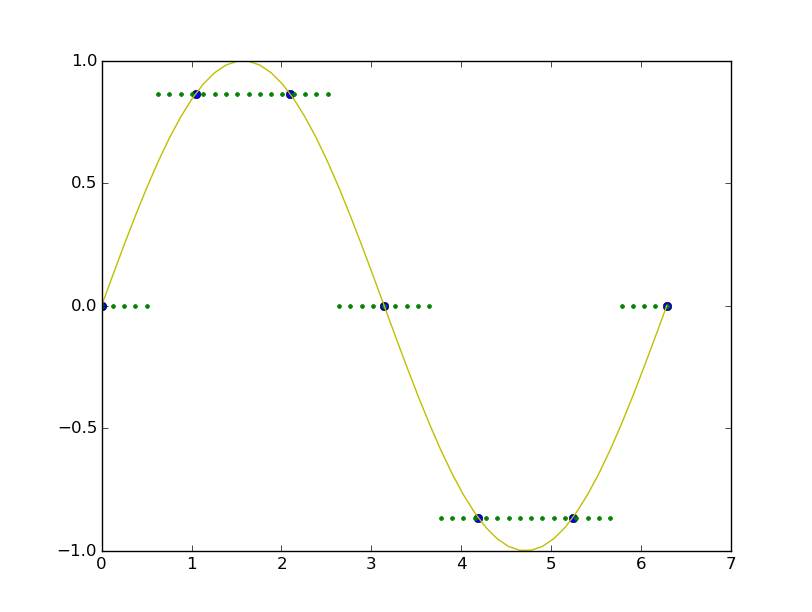
\includegraphics[width=0.32\textwidth,keepaspectratio=true]{./Interp0.png}
 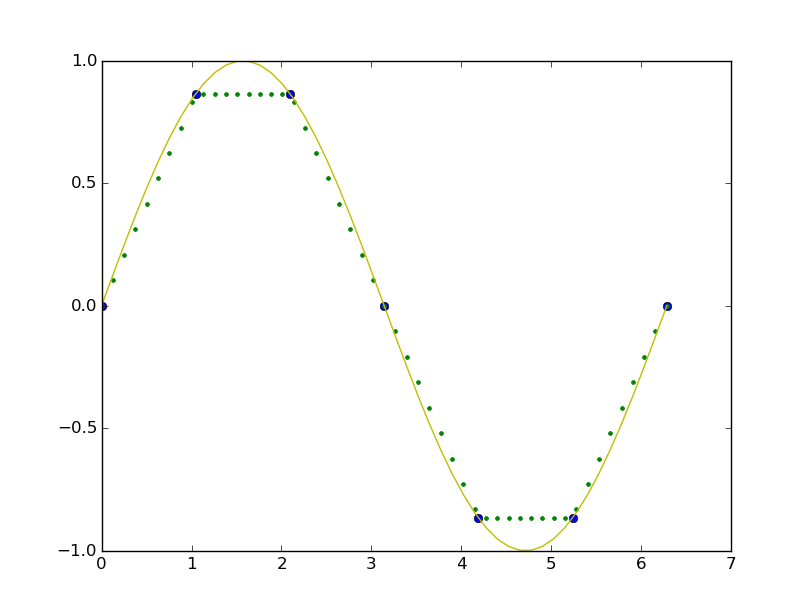
\includegraphics[width=0.32\textwidth,keepaspectratio=true]{./Interp1.png}
 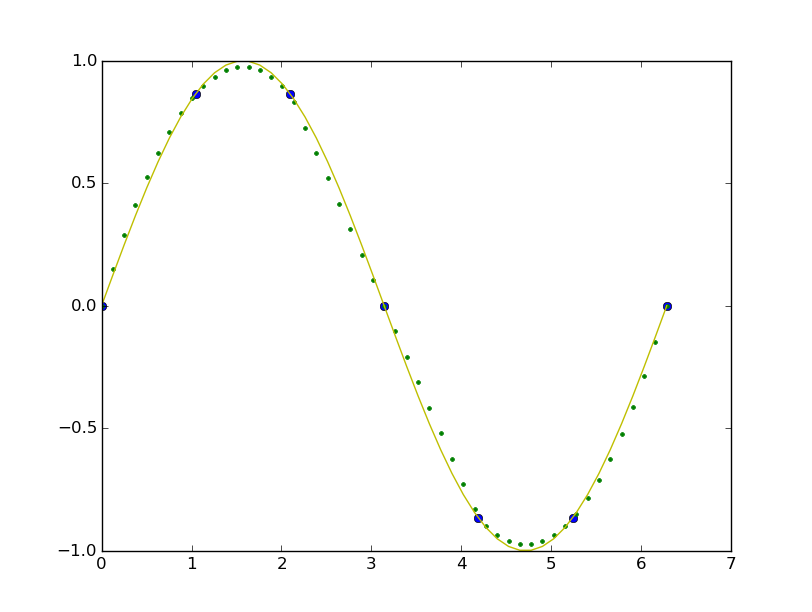
\includegraphics[width=0.32\textwidth,keepaspectratio=true]{./Interp2.png}
 \caption{Starting with the $\sin(x)$ defined at only 7 points (blue dotes), we calculate the (a) constant (rectangle) (b) linear (trapezoidal) and (c) quadratic interpolation points (green dots). In both panels the yellow lines show the exact $\sin(x)$ for comparison.}
 \label{fig:interp}
\end{figure}


\subsection*{Linear interpolation}

Say you have a finite set of points $\{x_n\}$ labeled by the integer $0 \leq n \leq N$, and you known the function $f(x)$ at these points. You may use the data from the example above with $f(x) = sin(x)$, or any other function of your choice.

Now, assume you want the value of the function at an general point $x$ that does not belong to your discrete set $\{x_n\}$, but lies within $x_a \leq x \leq x_b$. Here $b=a+1$ labeling consecutive points of the set. The most general expression for a linear interpolation connecting the points $\{x_a, f(x_a)\}$ and $\{x_b, f(x_b)\}$ is $\tilde{f}(x) = C_1 x+C_0$. We'll use the $\sim$ symbol to refer to the interpolated function. We want  $\tilde{f}(x)$ to match $f(x)$ at $x_a$ and $x_b$, therefore we have

\begin{align}
 \tilde{f}(x_a) &= C_1 x_a + C_0 = f(x_a),\\
 \tilde{f}(x_b) &= C_1 x_b + C_0 = f(x_b),
\end{align}
which defines a system of two equations and two unknowns ($C_1$ and $C_0$). This set of equations can be cast in a matrix form $M\cdot C = F$, where the matrix $M$, coefficient vector $C$ and function vector $F$ are show explicitly below:

\begin{equation}
 \begin{pmatrix}
  x_a & 1\\
  x_b & 1
 \end{pmatrix}
 \begin{pmatrix}
  C_1 \\ C_0
 \end{pmatrix}
 =
 \begin{pmatrix}
  f(x_a) \\ f(x_b)
 \end{pmatrix}.
\end{equation}

This equation can be easily solved as $C = M^{-1}\cdot F$. Evidently, you are able to express the result with paper \& pencil in this case. However, the matrix form makes it easy to generalize to higher order interpolation. The next example shows a code for linear interpolation, see Fig.~\ref{fig:interp}(a). In Problem \ref{prob:interpolation} I ask you to generalize this code for a quadratic interpolation that should result in Fig.~\ref{fig:interp}(b). 

As you can see, the quadratic interpolation is already very close to the exact $\sin(x)$ function. The interpolations usually work well because we are almost always dealing with analytical functions, smooth functions. Complicated functions will probably require advanced methods. For instance, functions with singularities.

\begin{example}{Code for Linear Interpolation}
\label{ex:quadraticinterp}
\begin{minted}{julia}
using PyPlot

xlst = linspace(0, 2pi, 7); # create data for the example
flst = sin(xlst);

# receives number of points n (odd) to interpolate
# and the original data via x and f
function interp1(n, x, f)
    xnew = linspace(x[1], x[end], n); # creates new axes
    fnew = zeros(n); # and initialize new data as zero

    i = 1; # label new sites
    for j=1:(length(x)-1) # runs over old sites
        xa = x[j]; # known points
        xb = x[j+1];
        fa = f[j]; # known data
        fb = f[j+1];
        
        # matrix form to find the coefficients
        M = [xa 1.0; xb 1.0];
        C1, C0 = inv(M)*[fa; fb];

        # calculate the new data within every two points interval
        while i <= n && xnew[i] <= xb
            fnew[i] = C1*xnew[i] + C0;
            i += 1;
        end
    end
    return xnew, fnew; # return interpolated data
end

# calls function to interpolate
xnew, fnew = interp1(51, xlst, flst);

# plot old data, new data, and exact function
plot(xlst, flst, "o");
plot(xnew, fnew, "g.");
plot(xnew, sin(xnew), "y-");
\end{minted}
\end{example}



\section{Numerical Integration - Quadratures}

Common numerical integration schemes rely on simple interpolations (Newton–Cotes rules). Let's discuss these methods first. Later we give an overview of adaptive integration schemes, which is natively implemented in Julia as the function \texttt{quadgk}, and more sophisticated implementations for multi-dimensional integrals can be found on the \texttt{Cubature} package. We finish this section discussing the Monte Carlo integration technique.

\subsection{Polynomial Interpolations}

We have briefly discussed polynomial interpolations in the previous section. Now we'll use different interpolations to define common quadrature schemes. To establish a notation, we'll refer to the discrete points as $x_n$, where the integer $n$ labels the points as in Fig. ?. We'll assume that the set of points $\{x_n\}$ is equally spaced, so we can define a constant step $\Delta x = x_{n+1}-x_{n}$.

\subsection*{Rectangle rule}

The simplest quadrature method is the \textit{rectangle rule}. Here the function is assumed to be constant and equal to $f(x_n)$ within the interval $x_n-\Delta x/2 \leq x \leq x_n+\Delta x/2$. The interpolation resulting from this rule can be seen in Fig.~\ref{fig:interp}(a). Consequently, the integral over this range is

\begin{equation}
 \int_{x_n-\frac{\Delta x}{2}}^{x_n+\frac{\Delta x}{2}} f(x) dx \approx f(x_n) \Delta x + \mathcal{O}(\Delta x).
\end{equation}


\subsection*{Trapezoidal rule}

The trapezoidal rule uses the linear interpolation shown in Fig.~\ref{fig:interp}(b). It is easy to see (Prob.~\ref{prob:quadrature}) that this leads to 

\begin{equation}
 \int_{x_n}^{x_{n+1}} f(x) dx \approx \dfrac{f(x_{n+1}) + f(x_n)}{2}\Delta x + \mathcal{O}(\Delta x^2).
\end{equation}

\subsection*{Simpson's rule}

If we use the parabolic interpolation, we get Simpson's rule:

\begin{equation}
 \int_{x_n}^{x_{n+2}} f(x) dx \approx \Big[f(x_n) + 4 f(x_{n+1}) + f(x_{n+2})\Big] \dfrac{\Delta x}{3} + \mathcal{O}(\Delta x^4).
\end{equation}

From Fig.~\ref{fig:interp} one can already expect that the Simpson's rule to give better results and the rectangular or trapezoidal rules.

\subsection*{General remarks on the rules above}

Note that the trapezoidal rule is defined over a range set by two consecutive points, while the Simpson's rule runs over three points, from $x_n$ to $x_{n+2}$. As a consequence the Simpson's rule can only be used if you have an odd number of known points.

Higher order polynomials leads to more precise quadrature rules. Cubic interpolation leads to the Simpson's $3/8$ rule, which uses 4 points. For polynomial interpolations of degree 4 we get Boole's rule, which uses 5 points.

In the next example I assume we have a discrete set of points given by \texttt{xlst} and \texttt{flst} that correspond to the output of some previous calculation. The function \texttt{trapezoidal} is then used to integrate the function. Problem \ref{prob:SimpleIntegral} asks you to implement other rules. Try to change the number of points in the example, as well as other more complicated functions.

\begin{example}{Numerical quadrature of a discrete function}
\label{ex:numericalquadrature}
\begin{minted}{julia}
# receives two vectors for the axis x and function f
function trapezoidal(x, f)
   delta = x[2]-x[1]; # assuming constant step
   res = 0.0; # initializes the sum
   for n=1:(length(x)-1)
       res += 0.5*(f[n+1]+f[n])*delta; # traditional rule
   end
   return res; # returns the result
end

# create data for the example
xlst = linspace(0, 2pi, 7); # x axis
flst = sin(xlst); # discretized function f(x)

trapezoidal(xlst, flst) # calls the function and shows the result
\end{minted}
\end{example}

We may also need to integrate an exact function $f(x)$. This is done in the next example. Now the \texttt{trapezoildal} function receives the function to be integrated, the limits of integration, and the number of points to consider. Here the function is never written as a vector. Instead, it is calculated as needed. This will be more efficient for integration with a large number of points, as it doesn't store the function as the vector \texttt{flst} as above.

\begin{example}{Numerical quadrature of a function f(x)}
\label{ex:numericalquadrature2}
\begin{minted}{julia}
# receives the function g(x) to be integraded
# from x=a to x=b with n points
function trapezoildal(g, a, b, n)
   dx = (b-a)/(n-1.0);
   xi(i) = a + (i-1.0)*dx;
   res = 0.0;	
   for i=1:(n-1)
      res += 0.5*(g(xi(i+1))+g(xi(i)))*dx
   end
   return res;
end

f(x) = sin(x); # chosen function

trapezoildal(f, 0, pi, 3) # test with 3 points

trapezoildal(f, 0, pi, 20) # 20 points

trapezoildal(f, 0, pi, 100) # 100 points
\end{minted}
\end{example}

Note that these examples illustrate two distinct cases. In Example \ref{ex:numericalquadrature} we assume that some previous calculation has given us the axis discretized into the vector \texttt{xlst} as well as the function \texttt{f(x)} calculated at these points and stored in the vector \texttt{flst}. This means that we are assuming that we don't have direct access to an exact function \texttt{f(x)}. 

Example \ref{ex:numericalquadrature2} presents the opposite case. Here we do have access to the exact function \texttt{f(x)}. In this case one may use more sophisticated quadrature schemes. We present some of them in the next section.

\subsection{Adaptive and multi-dimensional integration}

Julia already has a native quadrature code implemented (\texttt{quadgk}). It uses an adaptive Gauss-Kronrod integration technique. Since this is an introductory class, I will not go into details of this method\footnote{Those who are interested in mode details, please check the Wikipedia page for Adaptive quadrature and references within: \url{https://en.wikipedia.org/wiki/Adaptive_quadrature}}. 

But to get an idea of how the code works, imagine you have two quadrature of different order implemented, say the trapezoidal and Simpson's rules, and you want to integrate \texttt{f(x)} from \texttt{x=a} to \texttt{x=b}. First you split your integration into subintervals, say from \texttt{x=a} to \texttt{x=c}, and from \texttt{x=c} to \texttt{x=b}, \textit{i.e.}

\begin{equation}
 \int_a^b f(x) dx = \int_a^c f(x) dx + \int_c^b f(x) dx.
\end{equation}
Then you evaluate each integral on the right hand side independently. You can estimate the error of each subinterval comparing the result of the  trapezoidal and Simpson's rules. If the error of a subinterval is too big, you split it into a new pair of subintervals and repeat the test until you converge to the desired error.

An efficient implementation of such methods can be difficult, and I leave it as a challenge for the experienced programmers in Problem \ref{prob:adaptive}.

Luckily, Julia has already the function \texttt{quadgk}. Check its documentation for details on the parameters. The next example shows a basic usage.

\begin{example}{Numerical quadrature with \texttt{quadgk}}
\label{ex:quadgk}
\begin{minted}[mathescape]{julia}
# let's start with the same function from the previous example
f(x) = sin(x);
# quadgk receives the function and the limits of integration
quadgk(f, 0, pi)

# you may also try functions with integrable singularities...
f(x) = 1/sqrt(x);
quadgk(f, 0, 16) # exact result is 8

# and integrate all the way to infinity (Inf)
f(x) = exp(-(x^2)/2)/sqrt(2);
res = quadgk(f, -Inf, Inf) # exact result is $\sqrt{\pi}$
pi-res[1]^2 # compare to $\pi$ to check the error
\end{minted}
\end{example}

For more advanced routines and multi-dimensional integration, please check Julia's \texttt{Cubature} package\footnote{Cubature package: \url{https://github.com/stevengj/Cubature.jl}}.

\subsection{Monte Carlo integration}

While the previous methods integrate functions sampling them along a regular grid, the Monte Carlo integration scheme samples the integration interval using random numbers. We have used this method already to calculate $\pi$ back in Problem \ref{prob:pi}, which can be recast as a two-dimensional integral:

\begin{equation}
 f(x,y) =
   \begin{cases} 
   4  & \text{if } x^2+y^2 \leq 1, \\
   0  & \text{otherwise,}
  \end{cases}
\end{equation}

\begin{equation}
 \pi = \int_\Omega f(x,y) dx dy,
\end{equation}
where the integration area $\Omega$ is set by the ranges $0 \leq x \leq 1$ and $0 \leq y \leq 1$.

The Monte Carlo implementation of this integral reads

\begin{equation}
 R_N = \dfrac{1}{N} \sum_{i=1}^N f(x_i, y_i).
\end{equation}

The next example shows an implementation of this integral

\begin{example}{Monte Carlo integral to calculate $\pi$}
\label{ex:montecarlopi}
\begin{minted}[mathescape]{julia}
function Rn(f, n) # Monte Carlo integration of f(x,y)
   res=0.0;
   for i=1:n
      res += f(rand(), rand());
   end
   return res/n;
end

# define the function using the ternary operator
f(x,y) = (x^2+y^2 <= 1.0)?4.0:0.0;

Rn(f, 10) # run the integral with 10 points
Rn(f, 1000) # run the integral with 100 points
\end{minted}
\end{example}

The main advantage of the Monte Carlo integral is that its error decays with $1/\sqrt(n)$ independently of the dimensions of the integral. Therefore this method becomes very interesting for high-dimensional integrals.

\section{Numerical Derivatives}

At the beginning of this Chapter, our overview of the numerical calculus introduced the idea of a numerical derivative simply as dropping the infinitesimal limit on the definition of a derivative. Indeed this leads to a familiar expression:

\begin{equation}
 \dfrac{\partial f(x)}{\partial x} = \lim_{\Delta x \rightarrow 0} \dfrac{f(x+\Delta x) - f(x)}{\Delta x} \approx \dfrac{f(x+\Delta x) - f(x)}{\Delta x}.
\end{equation}
As far as $\Delta x$ is small, this should give us a good estimate of the derivative. This formula is actually known as the \textbf{forward} derivative, as it gives the derivative of $f(x)$ at $x$ using two points: $x$ itself, and the one step forward $x+\Delta x$.

\subsection{Finite differences and Taylor series}

The finite differences scheme is the most common method for numerical differentiation. Its arises from the Taylor expansion of a function $f(x)$:

\begin{equation}
 f(x_i+h) = f(x_i) + h \left.\dfrac{\partial f}{\partial x}\right|_{x_i} + \dfrac{h^2}{2!}\left.\dfrac{\partial^2 f}{\partial x^2}\right|_{x_i}
 +\dfrac{h^3}{3!}\left.\dfrac{\partial^3 f}{\partial x^3}\right|_{x_i} + \cdots
 \label{eq:fwdTaylor}
\end{equation}
Here $x_i$ is an arbitrary point of our discrete grid labeled by the integer $i$, and $h$ is the step size between discrete points.

Let's use the Taylor expansion to get the $1^{st}$ and $2^{nd}$ derivatives of $f(x)$ using two or three points of the discrete axis $x \rightarrow x_i$.

\subsection*{Forward $1^{st}$ derivative}

If we truncate the Taylor expansion on the $h^2$ term, we can rearrange the remaining terms to read:

\begin{equation}
 \left.\dfrac{\partial f}{\partial x}\right|_{x_i} \approx \dfrac{f(x_i+h) - f(x_i)}{h} + \mathcal{O}(h)
\end{equation}

\subsection*{Backward $1^{st}$ derivative}

Another choice is to start with the Taylor expansion for a negative step

\begin{equation}
 f(x_i-h) = f(x_i) - h \left.\dfrac{\partial f}{\partial x}\right|_{x_i} + \dfrac{h^2}{2!}\left.\dfrac{\partial^2 f}{\partial x^2}\right|_{x_i}
 -\dfrac{h^3}{3!}\left.\dfrac{\partial^3 f}{\partial x^3}\right|_{x_i} + \cdots
 \label{eq:bwdTaylor}
\end{equation}
and once again truncate the expansion on the $h^2$ term to get

\begin{equation}
 \left.\dfrac{\partial f}{\partial x}\right|_{x_i} \approx \dfrac{f(x_i) - f(x_i-h)}{h} + \mathcal{O}(h)
\end{equation}

\subsection*{Symmetric (or central) $1^{st}$ derivative}

Subtracting Eq.~\eqref{eq:fwdTaylor} from Eq.~\eqref{eq:bwdTaylor} we eliminate the $h^2$ term

\begin{equation}
 f(x_i+h) - f(x_i-h) = 2h \left.\dfrac{\partial f}{\partial x}\right|_{x_i} + 2\dfrac{h^3}{3!}\left.\dfrac{\partial^3 f}{\partial x^3}\right|_{x_i} + \cdots
\end{equation}
and now we can truncate the sum on the $h^3$ term to get

\begin{equation}
 \left.\dfrac{\partial f}{\partial x}\right|_{x_i} \approx \dfrac{f(x_i+h) - f(x_i-h)}{2h} + \mathcal{O}(h^2)
\end{equation}


\subsection*{Symmetric (or central) $2^{nd}$ derivative}

This time let's sum Eqs.~\eqref{eq:fwdTaylor} and \eqref{eq:bwdTaylor} to eliminate the first derivative:

\begin{equation}
 f(x_i+h) + f(x_i-h) = 2f(x_i) + h^2\left.\dfrac{\partial^2 f}{\partial x^2}\right|_{x_i} + \cdots
\end{equation}
Rearranging the expansion truncated on the $h^4$ term give us

\begin{equation}
 \left.\dfrac{\partial^2 f}{\partial x^2}\right|_{x_i} \approx \dfrac{f(x_i+h) - 2f(x_i) + f(x_i-h)}{h^2} + \mathcal{O}(h^2)
\end{equation}

Run the next example to get a plot comparing the first derivatives with the exact result. Try changing the step size from \texttt{h=pi/5} to \texttt{pi/50} and \texttt{pi/500}.

\begin{example}{Derivative using finite differences}
\label{ex:finitedifferences}
\begin{minted}[mathescape]{julia}
# simple implementation of the finite differences
diff1_forward(f, x, h) = (f(x+h)-f(x))/h;
diff1_backward(f, x, h) = (f(x)-f(x-h))/h;
diff1_symmetric(f, x, h) = (f(x+h)-f(x-h))/(2h);

f(x) = sin(x); # chosen function to test

xgrid = 0:(pi/50):pi; # discrete x axis
h = pi/5; # step for the derivatives

# using comprehensions to calculate the derivatives along xgrid
fwd = [diff1_forward(f, x, h) for x=xgrid]
bwd = [diff1_backward(f, x, h) for x=xgrid]
sym = [diff1_symmetric(f, x, h) for x=xgrid]

# plot the exact result and the approximate derivatives for comparison
clf();
plot(xgrid, cos(xgrid); label="cos(x)")
plot(xgrid, fwd; label="forward")
plot(xgrid, bwd; label="backward")
plot(xgrid, sym; label="symmetric")
legend()
\end{minted}
\end{example}

In the example above we are assuming that we have access to the exact function $f(x)$ at any point. This is similar to what we saw in Example \ref{ex:numericalquadrature2}. What happens if we consider a situation similar to the one in Example \ref{ex:numericalquadrature}? There we assume that we only known the function $f(x)$ via the discrete points set by \texttt{xlst} and \texttt{flst}. Check \mbox{Problem \ref{prob:finitediff2}.}

\subsection{Matrix Representation}
\label{sec:matrixrepresentation}

Sometimes it is useful to represent the derivatives in matrix forms, such that it becomes an operator. Say that we have a discrete $x$ axis labeled by $x_i$ for $1 \leq i \leq N$, and a function defined at these points by $f_i = f(x_i)$. These are exactly the \texttt{xlst} and \texttt{flst} vectors from the previous Examples of this Chapter. Let's assume that $f_i = 0$ for $i \leq 0$ and $i \geq N+1$. Let's write the expressions for the symmetric finite differences derivative $f'_i = \left.\frac{\partial f(x)}{\partial x}\right|_{x_i}$ at each point $x_i$:

\begin{align}
 \text{for i=1, }\quad f'_1 &= \dfrac{f_2-0}{2h},\\
 \text{    i=2, }\quad f'_2 &= \dfrac{f_3-f_1}{2h},\\
 \text{    i=3, }\quad f'_3 &= \dfrac{f_4-f_2}{2h},\\
 \text{    i=4, }\quad f'_4 &= \dfrac{f_5-f_3}{2h},\\
          \cdots \quad f'_i &= \dfrac{f_{i+1}-f_{i-1}}{2h},\\
 \text{  i=N-1, }\quad f'_{N-1} &= \dfrac{f_N-f_{N-2}}{2h},\\
 \text{  i=N,   }\quad f'_{N} &= \dfrac{0-f_{N-1}}{2h}.
\end{align}
The zero in the first and last lines refer to $f_0 = 0$ and $f_{N+1} = 0$, respectively.

The set of equations above can be put in a matrix form as

\begin{equation}
 \begin{pmatrix}
  f'_1 \\f'_2 \\ f'_3 \\ f'_4 \\ \cdots \\ f'_i \\ \cdots \\ f'_{N-1} \\ f'_N
 \end{pmatrix}
 = \dfrac{1}{2h}
\begin{pmatrix} 
 0 & 1 & 0 & 0 & 0 & 0 & 0 & 0 & 0\\
 -1 & 0 & 1 & 0 & 0 & 0 & 0 & 0 & 0\\
 0 & -1 & 0 & 1 & 0 & 0 & 0 & 0 & 0\\
 0 & 0 & -1 & 0 & 1 & 0 & 0 & 0 & 0\\
 0 & 0 & 0 & -1 & 0 & 1 & 0 & 0 & 0\\
 0 & 0 & 0 & 0 & -1 & 0 & 1 & 0 & 0\\
 0 & 0 & 0 & 0 & 0 & -1 & 0 & 1 & 0\\
 0 & 0 & 0 & 0 & 0 & 0 & -1 & 0 & 1\\
 0 & 0 & 0 & 0 & 0 & 0 & 0 & -1 & 0
\end{pmatrix}
\begin{pmatrix}
  f_1 \\f_2 \\ f_3 \\ f_4 \\ \cdots \\ f_i \\ \cdots \\ f_{N-1} \\ f_N
\end{pmatrix}
\end{equation}

In Julia this matrix can be implemented using the \texttt{diagm} function:

\begin{example}{Matrix representation of the first derivative}
\label{ex:matrix}
\begin{minted}[mathescape]{julia}
x = linspace(-10, 10, 101); # discrete x axis
f = exp(-(x.^2)/2.0); # function sampled at x

n = length(x); # number of points
h = x[2] - x[1]; # step size

matdiff = (diagm(ones(n-1), 1) - diagm(ones(n-1), -1))/(2h);

# calculates the derivative of f as a product of matrix and vector
dfdx = matdiff*f; 

plot(x, dfdx);
\end{minted}
\end{example}

\subsection{Derivatives via convolution with a kernel}

A one-dimensional (1D) discrete convolution of the vectors \texttt{f} and \texttt{g} read

\begin{equation}
 (g \ast f)[n] = \sum_{m=1}^N g[m]f[n+N-1-m],
\end{equation}
where the index of our arrays $g[m]$ and $f[m]$ start at 1 and $N$ is the length of the array $g$.



Let's refer to the vector \texttt{g} as the kernel, and \texttt{f} as our function. If the kernel is \mbox{$g = \frac{1}{2h}(1, 0, -1)$}, the convolution above becomes

\begin{equation}
 (g \ast f)[n] = \dfrac{1}{2h}\Big(f[n+1] - f[n-1]\Big),
\end{equation}
which is exactly our definition of the symmetric first derivative. 

In Julia we can use the \texttt{conv} function for 1D convolutions and the \texttt{conv2} function for two-dimensional (2D) convolutions. The next example can be compared with the previous one. Note that after the convolution we remove end points to keep \texttt{dfdx} with the same size of \texttt{x}.

\begin{example}{Derivatives via convolution with a kernel 1D}
\label{ex:conv}
\begin{minted}[mathescape]{julia}
x = linspace(-10, 10, 101); # discrete x axis
f = exp(-(x.^2)/2.0); # function sampled at x

n = length(x); # number of points
h = x[2] - x[1]; # step size

# kernel for the symmetric first derivative 1D
kernel = [1.0; 0.0; -1.0]/(2h);

dfdx = conv(kernel, f); # convolution
dfdx = dfdx[2:end-1]; # remove end points

plot(x, dfdx);
\end{minted}
\end{example}

In 2D the kernel becomes a matrix. For instance, the kernel for $\frac{\partial^2}{\partial x \partial y}$ represented by the symmetric differences with step sizes $h_x$ and $h_y$ in each direction is

\begin{equation}
 g = \dfrac{1}{4 h_x h_y}
 \begin{pmatrix}
  0 & 1 & 0 \\
  1 & 0 & -1 \\
  0 & -1 & 0
 \end{pmatrix}.
\end{equation}

\begin{example}{Derivatives via convolution with a kernel 2D}
\label{ex:conv2}
\begin{minted}[mathescape]{julia}
# x and y axes
# transpose y to get matrix mesh for f later on
x = linspace(-5, 5, 101);
y = transpose(linspace(-5, 5, 101));
hx = x[2]-x[1]; # step sizes
hy = y[2]-y[1];

# 2D function as a matrix (lines are x, columns are y)
f = exp(-(x.^2)/2).*exp(-(y.^2)/2);

# 2D kernel for $\frac{\partial^2}{\partial x \partial y}$
kernel = (1.0/(4*hx*hy))*[0.0 1.0 0.0; 1.0 0.0 -1.0; 0.0 -1.0 0.0];

df = conv2(kernel, f); # 2D convolution
df = df[2:end-1, 2:end-1]; # remove end points

surf(x, y', df) # surface plot
# requires y to be transposed back into a column vector
\end{minted}
\end{example}


\subsection{Other methods, Julia commands and packages for derivatives}

Later on we'll see how to take derivatives using the properties of Fourier transforms. This will be useful to solve differential equations, for instance with the split-operator or split-step methods.

Julia has a native command for the first order derivatives: \texttt{gradient}. This command uses the forward rule to evaluate the derivative at the first point, the backward rule at the last point, and the symmetric rule at the internal points.

There exists also packages, like the \texttt{ForwardDiff}\footnote{ForwardDiff package: \url{https://github.com/JuliaDiff/ForwardDiff.jl}}. However there's a warning on the webpage of \texttt{ForwardDiff} and at this moment I'm not familiarized with the issues they are facing.

\section{Problems}

\begin{problem}{Checking the simplest numerical integration}
 \label{prob:SimpleIntegral}

 Consider the functions $f(x) = \sin(x)$, $g(x) = \cos(x)$, and $h(x) = e^x$.
 
 \textbf{a)} What is the exact result for the integration of $f(x)$ and $g(x)$ on the interval $0 \leq x \leq 2\pi$? Try also the interval $0 \leq x \leq \pi$. What about the integration of $h(x)$ over $0 \leq x \leq 1$?
 
 \textbf{b)} Try to numerically integrate these functions as initially described at the introduction of this chapter. Simply dropping the infinitesimal limit. Compare the deviation from the exact result as a function of the number of points used in the integration in a log-plot. Useful Julia commands: \texttt{linspace}, \texttt{sum}.
 
 \textbf{c)} Complement item \textbf{(b)} as you learn new methods: compare the precision of different methods (trapezoidal, Simpson's, Boole's, Monte Carlo, ...) as a function of the number of points being used.
 
\end{problem}

\begin{problem}{Interpolation}
 \label{prob:interpolation}
 
 Go back to Example \ref{ex:quadraticinterp}, which shows a code for a linear interpolation $\tilde{f}(x) = C_1 x + C_0$. Following the example, implement (a) a code to get a quadratic interpolation $\tilde{f}(x) = C_2 x^2 + C_1 x + C_0$, (b) a code for the rectangle interpolation. You must reproduce Fig.~\ref{fig:interp}.
 
\end{problem}

\begin{problem}{Quadrature equations}
 \label{prob:quadrature}

 (a) Show that the linear interpolation leads to the trapezoidal quadrature rule.
 
 (b) Show that the quadratic interpolation leads to the Simpson's rule.
\end{problem}

\begin{problem}{Adaptive Integration}
 \label{prob:adaptive}
 
 This problem might not be easy. I'll leave it here as a challenge for the more experienced programmers among the students: Try to implement an adaptive integration code using the trapezoidal and Simpson's rule discussed in the text.
 
\end{problem}

\begin{problem}{Monte Carlo integration and $\pi$}
 \label{prob:montecarlopi}

Edit the Monte Carlo Example \ref{ex:montecarlopi} or your code from Problem \ref{prob:pi} to calculate $\pi$ as a function of the number $n$ of randomly sampled points. Let's say that $R_n$ is the result of the calculation with $n$ points. The relative error is $E_n = (R_n-\pi)/\pi$. Do a log-log plot of $E_n$ vs $n$ to see that the error goes with $1/\sqrt(n)$, which is the typical behavior of Monte Carlo integrals.
\end{problem}

\begin{problem}{Derivatives via finite differences with an exact function}
 \label{prob:finitediff}

 \textbf{(a)} Following Example \ref{ex:finitedifferences}, write a code to calculate the second derivative of a function $f(x)$ and compare with the exact result.
 
 \textbf{(b)} Run the Example \ref{ex:finitedifferences} and the code you wrote on item (a) with the following functions
 
 \begin{itemize}
  \item $f(x) = e^{-x^2}$, for $-5 < x < 5$;
  \item $f(x) = \sqrt{x}$, for $0 < x < 10$;
  \item $f(x) = 4x^4 + 3x^3 + 2x^2 + x$, for $-10 < x < 10$.
 \end{itemize}
\end{problem}


\begin{problem}{Derivatives via finite differences with a discrete axis}
 \label{prob:finitediff2}

 Let's assume that we only have the function $f(x)$ sampled at discrete points set by \texttt{xlst} and stored at the vector \texttt{flst}:
 
 \begin{minted}[mathescape]{julia}
  h = pi/5; # grid step
  xlst = 0:h:pi; # discrete x axis
  flst = sin(xlst); # function evaluated at discrete points
 \end{minted}

 \textbf{(a)} Write a code to calculate the first and second derivatives using this discrete data. Here the derivative step size has to be equal to the grid step size. You will face a difficulty at the end points. What can you do?
 
 \textbf{(b)} Test your code with the functions of the previous Problem. Try to vary the grid step to see how the precision changes.

\end{problem}


\begin{problem}{Matrix representation of the finite differences}
 \label{prob:matrix}

 Following Example \ref{ex:matrix}, implement the matrix representation for the finite differences derivatives:
 
 \textbf{(a)} First derivative: forward, backward and symmetric. Change the step size trying to visualize the difference between these implementations.
 
 \textbf{(b)} Second derivative: symmetric.
 
 Always test your implementations with well known functions that you can differentiate analytically for comparison.
 
\end{problem}


\begin{problem}{Derivatives via convolution with a kernel}
 \label{prob:kernel}

 Implement the forward and backward first derivatives, and the second symmetric derivative in 1D using convolution with a kernel following the Example \ref{ex:conv}.
 
\end{problem}














\chapter{Ordinary Differential Equations}

\vspace*{-1cm}
\begin{flushright}
\texttt{ENIAC, since 1946}
\end{flushright}

\lettrine[nindent=0.35em,lhang=0.40,loversize=0.3]{E}{NIAC}, \textbf{E}lectronic \textbf{N}umerical \textbf{I}ntegrator \textbf{A}nd \textbf{C}omputer\cite{haigh2016eniac},
the first electronic general-purpose computer was designed by the US Army and finished in 1946\footnote{ENIAC: \url{https://en.wikipedia.org/wiki/ENIAC}}. The goal was to numerically calculate artillery firing tables by solving sets of differential equations. Essentially, $\bm{F} = m\bm{a}$ with quite a few complications.

Indeed we are surrounded by differential equations...

\begin{equation}
 m \dfrac{\partial^2 \bm{r}}{\partial t^2} = \bm{F},
\end{equation}

\begin{equation}
 i\hbar \dfrac{\partial \psi(\bm{r},t)}{\partial t} = H \psi(\bm{r},t),
\end{equation}

\begin{equation}
 \begin{array}{c c c c}
  \bm{\nabla}\cdot\bm{D} = \rho, \quad & \bm{\nabla}\cdot\bm{B} = 0, \quad & \bm{\nabla}\times\bm{E} = -\dfrac{\partial \bm{B}}{\partial t}, \quad & \bm{\nabla}\times\bm{H} = \dfrac{\partial \bm{D}}{\partial t} + \bm{J},
 \end{array}
\end{equation}

\begin{equation}
 \dfrac{\partial u}{\partial t} -\alpha^2 \bm{\nabla}^2 u = 0,
\end{equation}

\begin{equation}
 \dfrac{\partial^2 u}{\partial t^2} - c^2 \bm{\nabla}^2 u = 0,
\end{equation}

... to list a few. We also have Navier–Stokes, general relativity, etc.

The unknown quantity in a differential equation can be a function of a single variable, like the position that depends on time on Newton's second law above ($\bm{r} \equiv \bm{r}(t)$). These cases are labeled \texttt{ordinary differential equations} (ODE). If your function depends upon two or more variables and your differential equation has derivatives on these variables, it becomes a \texttt{partial differential equation} (PDE). This is the case of all other examples above. PDEs and ODEs are intrinsically different. Important theorems of ODEs do not apply for PDEs.

Let us compare two simple cases, the Laplace equation in one and two dimensions:

\begin{align}
 \dfrac{\partial^2 f(x)}{\partial x^2} &= 0,\\
 \left(\dfrac{\partial^2}{\partial x^2} + \dfrac{\partial^2}{\partial y^2}\right)f(x,y) &= 0.
\end{align}

The 1D equation is a second order ODE. This means that its most general solution is defined up to two unknown constants. These are set by two initial or boundary conditions. In this case the general solution is a straight line,

\begin{equation}
 f(x) = c_1x + c_0,
\end{equation}
where $c_1$ and $c_0$ are the unknown coefficients.

Contrasting the simplicity of the 1D Laplace equation, the 2D version, which is a PDE, has an infinite number of solutions. Introducing complex variables, it is easy to verify that the most general solution is

\begin{equation}
 f(x,y) = p(z) + q(\bar{z}),
\end{equation}
where $p(z)$, $q(\bar{z})$ are arbitrary analytical functions of the complex variables $z = x+iy$, $\bar{z} = x-iy$.

For now, we will focus on \texttt{ordinary differential equations} (ODE). These can be classified into three main categories: (i) initial value problems; (ii) boundary-value problems; and (iii) eigenvalue problems. Here we shall restrict ourselves to introductory discussion on the methods to solve ODEs, for more details please check Ref.~\cite{JCButcher2008NumericalODE, pang2006introduction}.


\section{Initial value problem: time-evolution}

Initial value problems usually deal with the dynamics of a system, where the derivatives are taken with respect to time. Newton's second law is the paradigmatic example of an initial value ODE,

\begin{equation}
 \dfrac{d^2 \bm{r}}{dt^2} = \dfrac{\bm{F}}{m},
\end{equation}
requiring the \texttt{initial} position $\bm{r}(0)$ and velocity $\bm{v}(0)$ to be solved.

Let's consider the one dimensional case to guide our discussion. Just keep in mind that a generalization to more dimensions is immediate. First we write Newton's second law in a more general form of an arbitrary second order initial value problem ODE,

\begin{equation}
 \dfrac{d^2 x}{dt^2} = g(x,t).
\end{equation}

This second order ODE can be split into a pair of coupled first order ODEs using $v = \frac{dx}{dt}$, yielding

\begin{equation}
 \dfrac{dv}{dt} = g(x,t), \quad \text{ and } \quad \dfrac{dx}{dt} = v.
\end{equation}

Finally, we can define vectors $\bm{y} = [ v(t), x(t) ]$ and $\bm{f} = [ g(x,t), v(t) ]$, such that the equations above can be cast as

\begin{equation}
 \dfrac{d \bm{y}}{dt} = \bm{f}.
 \label{eq:dydteqf}
\end{equation}


\subsection*{Example: the pendulum}

Any physics text-book will tell you that the equation of motion for the pendulum is

\begin{equation}
 \dfrac{d^2\theta(t)}{dt^2} = -\omega^2 \sin[\theta(t)],
 \label{eq:pendulum}
\end{equation}
where $\theta(t)$ is the angular displacement, $\omega^2 = g/\ell$, $g \approx 9.8$~m/s$^s$ is the gravity, and $\ell$ is the pendulum length.

For small oscillations we can use Taylor's expansion to write $\sin\theta \approx \theta$. This leads to the usual harmonic solution $\theta(t) = A\cos(\omega t + \phi)$, where the amplitude $A$ and the phase constant $\phi$ are set by initial conditions.

Let us try to go beyond the small oscillations approximation and numerically solve Eq.~\eqref{eq:pendulum} with the content of the next sections. To do this, first we have to rewrite Eq.~\eqref{eq:pendulum} in the form of a set of coupled first order ODEs as we generically did above. With this purpose, define\footnote{Within the text I'll use the dot notation to refer to time derivatives, \textit{i.e.} $\dot{\theta} = \dfrac{d\theta}{dt}$} $x(t) = \theta(t)$ and $v(t) = \dot{\theta}(t)$. The pendulum equation of motion becomes

\begin{equation}
 \dfrac{dv}{dt} = -\omega^2\sin[\theta(t)],  \quad \text{ and } \quad \dfrac{dx}{dt} = v,
 \label{eq:pendulumsplit}
\end{equation}
which can be cast as Eq.~\eqref{eq:dydteqf} setting $\bm{y} = [\dot{\theta}(t), \theta(t)]$ and $\bm{f} = [-\omega^2\sin[\theta(t)], \dot{\theta}(t)]$. To solve these equations we will have to specify the initial position $x(0)$ and velocity $v(0)$.

In the next sections we will learn methods to solve differential equations and apply them to this pendulum example. Note that replacing $\sin\theta \rightarrow \theta$ in Eq.~\eqref{eq:pendulumsplit} allows you to compare the results with the exact solution for small oscillations. Once you have confidence that your code works, put back the full $\sin\theta$ dependence and compare the small oscillations solution with the numerical solution for large amplitudes.

\subsection{The Euler method}

Go back to the previous Chapter and check the expression for the forward first derivative. Applying it to Eq.~\eqref{eq:dydteqf} gives

\begin{equation}
 \dfrac{\bm{y}(t+\tau) - \bm{y}(t)}{\tau} = \bm{f}(t),
\end{equation}
where $\tau$ is the discrete time step. Labeling the discrete time $t_n = t_0 + n\tau$ with integers $n$, we can define $\bm{y}(t_n) = \bm{y}_n$ and $\bm{f}(\bm{y}_n, t_n) = \bm{f}_n$. Rewriting the equation above give us

\begin{equation}
 \bm{y}_{n+1} = \bm{y}_n + \tau \bm{f}_n.
 \label{eq:euler}
\end{equation}
Since in principle we known $\bm{y}_0$ and $\bm{f}_0$ (initial values), the equation above can be used to iterate the solution from $n=0$ to all $n$. The global error of the Euler method is $\mathcal{O}(\tau)$.

\begin{example}{Euler method - Pendulum}
\label{ex:euler}
\begin{minted}{julia}
using PyPlot

w = 2pi; # frequency, period for small oscillations T = 2pi/w
g(x,t) = -(w^2)*sin(x); # r.h.s. of Newton's 2nd law
f(x,v,t) = [g(x,t); v]; # r.h.s. of linearized ODE

x0 = 0.5pi; # initial angular displacement
v0 = 0.0; # inicial angular velocity
y0 = [v0; x0]; # initial vector for linearized ODE

tau = 1e-4; # time step
tspan = 0:tau:5; # time range

yt = y0; # we will store the data for each t in yt
y = y0; # y at current t for the calculation
for t=tspan[1:end-1]
    y = y + tau*f(y[2], y[1], t); # Euler iteration
    yt = [ yt y ]; # store solution for each time step
end
# data stored in lines, transpose to use with PyPlot
v = transpose(yt[1,:]); # first line is v(t)
x = transpose(yt[2,:]); # second line is x(t)

small = x0*cos(w*tspan); # exact solution for small oscillations

# plot numerical and exact solutions for comparison
clf(); 
plot(tspan, x; label="numerical");
plot(tspan, small; label="small oscillations");
legend();
\end{minted}
\end{example}

In the example above, the initial displacement of the pendulum is set by $-\pi < x_0 < \pi$. For $|x_0| \ll \pi$ you should see a good agreement with the exact solution for small oscillations. For large $|x_0| \lesssim \pi$ the numerical simulation will show plateaus as the pendulum slows down near $x_0 = \pm \pi$. However, to see this you will probably have to reduce $\tau$ to recover stability. Try to play with the parameters.

% To improve the Euler method one can use Picard iterations or the Predictor-Corrector methods, see Ref.~\cite{pang2006introduction}.

\subsection{Runge-Kutta Methods}

The Runge-Kutta methods are the most popular methods for solving ODE due to its high-precision and stability. These methods can be classified as predictor-corrector methods, see Ref.~\cite{pang2006introduction}. The most used version is the $4^\text{th}$ order Runge-Kutta method, or simply RK4. But let's start with the RK2 for simplicity.

\subsubsection*{$2^\text{nd}$ order Runge-Kutta method (RK2)}

Our prototype for a differential equation, Eq.~\eqref{eq:dydteqf}, can be written in a integral form as

\begin{equation}
 \bm{y}(t+\tau) = \bm{y}(t) + \int_{t}^{t+\tau} \bm{f}\Big(y(t'), t'\Big) dt'.
\end{equation}
If we approximate the integrand by a constant value evaluated at the lower limit of the integral, \textit{i.e.} $\bm{f}(y(t'), t') = \bm{f}(y(t), t)$, we get the Euler method again: $\bm{y}_{n+1} = \bm{y}_n + \tau \bm{f}_n$.

Instead, if we approximate the integrand by the midpoint, \textit{i.e.} $\bm{f}(y(t'), t') = \bm{f}(y(t+\tau/2), t+\tau/2)$, we get

\begin{equation}
 \bm{y}_{n+1} = \bm{y}_n + \tau \bm{f}\Big( \bm{y}_{n+\frac{1}{2}}, t_n+\frac{\tau}{2} \Big).
\end{equation}
But we don't known $\bm{y}_{n+1/2}$. To proceed, there's two possibilities:

\paragraph*{(i) The explicit RK2} is obtained using the Euler method to express $\bm{y}_{n+1/2} = \bm{y}_n + \frac{1}{2}\tau\bm{f}_n$, yielding

\begin{equation}
 \bm{y}_{n+1} = \bm{y}_n + \tau \bm{f}\Big( \bm{y}_n + \frac{\tau}{2}\bm{f}(\bm{y}_n, t_n),\; t_n+\frac{\tau}{2} \Big).
 \label{eq:explicitRK2}
\end{equation}

\paragraph*{(ii) The implicit RK2} is obtained if we use the midpoint rule to express $\bm{y}_{n+1/2} = \frac{1}{2}( \bm{y}_n + \bm{y}_{n+1} )$,

\begin{equation}
 \bm{y}_{n+1} = \bm{y}_n + \tau \bm{f}\Big( \frac{\bm{y}_n + \bm{y}_{n+1}}{2} ,\; t_n+\frac{\tau}{2} \Big).
 \label{eq:implicitRK2}
\end{equation}

Both version result in global errors $\mathcal{O}(\tau^2)$.

Notice that the \textbf{explicit RK2} is slightly more complicated than the Euler method, but still very similar: on the left hand side we have the unknown $\bm{y}_{n+1}$ at the next time step, and on the right hand side we have all quantities evaluated at the current time step. Therefore it is easy to generalize the Euler code from Example \ref{ex:euler} to implement the explicit RK2. 

In contrast, the \textbf{implicit RK2} has the unknown $\bm{y}_{n+1}$ on both sides of the equation. To solve Eq.~\eqref{eq:explicitRK2} one can use the \textit{fixed-point iteration} method. Start with an initial guess for $\bm{y}_{n+1}$, which could be from the Euler method: $\bm{y}_{n+1}^{[0]} = \bm{y}_n + \tau \bm{f}_n$. For now on the superscript $[k]$ in $\bm{y}_{n+1}^{[k]}$ refers to the level of the iteration. Then iterate the solution until convergence,

\begin{align}
 \bm{y}_{n+1}^{[0]} &= \bm{y}_n + \tau \bm{f}_n,\\
 \bm{y}_{n+1}^{[1]} &= \bm{y}_n + \tau \bm{f}\Big( \frac{\bm{y}_n + \bm{y}_{n+1}^{[0]}}{2} ,\; t_n+\frac{\tau}{2} \Big),\\
 \bm{y}_{n+1}^{[2]} &= \bm{y}_n + \tau \bm{f}\Big( \frac{\bm{y}_n + \bm{y}_{n+1}^{[1]}}{2} ,\; t_n+\frac{\tau}{2} \Big),\\
 &\vdots \\
 \bm{y}_{n+1}^{[k+1]} &= \bm{y}_n + \tau \bm{f}\Big( \frac{\bm{y}_n + \bm{y}_{n+1}^{[k]}}{2} ,\; t_n+\frac{\tau}{2} \Big).
\end{align}
Convergence is achieved for large $k$ when $\bm{y}_{n+1}^{[k+1]} - \bm{y}_{n+1}^{[k]}$ is sufficiently small.

It is also possible to solve Eq.~\eqref{eq:explicitRK2} using root-finding algorithms (e.g. Newton's method). Notice that the only unknown quantity is $\bm{y}_{n+1}$, so let's define an auxiliary function $\bm{R}(\bm{y}_{n+1})$,

\begin{equation}
 \bm{R}(\bm{y}_{n+1}) = \bm{y}_{n+1} - \bm{y}_n - \tau \bm{f}\Big( \frac{\bm{y}_n + \bm{y}_{n+1}}{2} ,\; t_n+\frac{\tau}{2} \Big),
\end{equation}
such that the possible solutions of Eq.~\eqref{eq:explicitRK2} are the roots of $\bm{R}(\bm{y}_{n+1}) = 0$.


\subsubsection*{Explicit $4^\text{th}$ order Runge-Kutta method (RK4)}

The RK4 method is by far the most popular method to solve ODEs. Its implementation is not much more complicated than the simples Euler method, but its precision is far superior with a global error $\mathcal{O}(\tau^4)$. The iteration rule for the RK4 is

\begin{align}
 \bm{k}_1 &= \bm{f}(\bm{y}_n, t_n),\\
 \bm{k}_2 &= \bm{f}\Big(\bm{y}_n + \frac{\tau}{2}\bm{k}_1, t_n + \frac{\tau}{2}\Big),\\
 \bm{k}_3 &= \bm{f}\Big(\bm{y}_n + \frac{\tau}{2}\bm{k}_2, t_n + \frac{\tau}{2}\Big),\\
 \bm{k}_4 &= \bm{f}\Big(\bm{y}_n + \tau \bm{k}_3, t_n + \tau\Big),\\
 \bm{y}_{n+1} &= \bm{y}_n + \dfrac{\tau}{6}\Big(\bm{k}_1 + 2\bm{k}_2 + 2\bm{k}_3 + \bm{k}_4\Big).
\end{align}

Since this is the most used method for differential equations, I will not show an implementation example here. Instead, I'll leave its implementation as a problem for the students.

\subsection{Stiff equations}

Stiff differential equations are those where the numerical solution require a step size excessively small when compared with the actual smoothness of the solution. Typically, a stiff equation solved with a large step size show spurious oscillations. 

A stiff differential equation can be as simple as

\begin{equation}
 \dfrac{d y(t)}{dt} = -15 y(t),
\end{equation}
which has an exact solution $y(t) = e^{-15 t}$ for the initial condition $y(0) = 1$. Note that $y(t) > 0$ for any $t > 0$. However, if you apply the Euler method with $f(y) = -15y$, you will get $y_{n+1} = y_n -15\tau y_n$. For a large $\tau$, the Euler method may give negative values for $y_{n+1}$. Indeed, if you solve this equation with the Euler method with a large $\tau$, you will get the spurious oscillations.

A better choice is to use the implicit RK2 method. In this particular case you can actually solve Eq.~\eqref{eq:implicitRK2} analytically for $y_{n+1}$ to obtain

\begin{equation}
 y_{n+1} = \dfrac{1 - \frac{15}{2}\tau}{1+\frac{15}{2}\tau} y_n.
\end{equation}

The next example compares the numerical solutions of this stiff equation obtained with the explicit and implicit RK2 methods. Try running it with different step sizes $\tau$ and compare the results.

\begin{example}{Stiff ODE, implicit vs explicit RK2 methods}
\label{ex:stiff1}
\begin{minted}[mathescape]{julia}
# explicit RK2 solver receives the right hand side function,
# initial (t0) and final (t1) times, time-step (tau),
# and initial condition (y0)
function explicitRK2(rhs, t0, t1, tau, y0)
   tspan = t0:tau:t1; # sets the time span
   y = y0; # stores solutions in y
   yt = y0; # yt is the auxiliary for the iterations
   for t=tspan[1:end-1]
      # explicit RK2 rule:
      yt = yt + tau*rhs(t+tau/2, yt+0.5*tau*rhs(t, yt));
      y = [ y; yt ]; # stores solutions
   end
   return tspan, y;
end

# does not need the rhs as it is implemented specifically
# for the ODE: dy/dt = -15y
function implicitRK2(t0, t1, tau, y0)
   tspan = t0:tau:t1;
   y = y0;
   yt = y0;
   for t=tspan[1:end-1]
      # explicit solution of the implicit rule for this particular ODE
      yt = yt*(1.0-15*tau/2.0)/(1.0+15*tau/2.0);
      y = [ y; yt ];
   end
   return tspan, y;
end

rhs(t,y) = -15*y; # defines the right hand side of the ODE
y0 = 1.0; # initial condition

tau = 1.0/10; # same tau for both methods
te, ye = explicitRK2(rhs, 0.0, 1.0, tau, y0); # calls explicit RK2
ti, yi = implicitRK2(0.0, 1.0, tau, y0); # calls implicit RK2

texact = 0:0.01:1;
exact = exp(-15*texact); # exact solution for comparison

clf(); # plot the results
plot(texact, exact; label="Exact");
plot(te, ye; label="Explicit");
plot(ti, yi; label="Implicit");
legend();
axis([0.0, 1.0, -1.5, 1.5]);
\end{minted}
\end{example}

A more complicated stiff ODE is

\begin{equation}
 \dfrac{d y(t)}{dt} = y^2(t) - y^3(t).
\end{equation}
If you put $f(y) = y^2-y^3$ into the implicit RK2 Eq.~\eqref{eq:implicitRK2}, you will have three roots. Which one should you use? In this case it is better to use the fixed-point iteration method.

In the next example implement the implicit RK2 method using the fixed-point iteration for an initial condition $y(0) = y_0$ within a time range $0 \leq t \leq 2/y_0$. For small $y_0$ the ODE become stiff and the solution will require a very small $\tau$ to converge. You may use the implementation of the explicit RK2 from the previous example to compare with the implicit RK2 again.

\begin{example}{Stiff ODE, implicit vs explicit RK2 methods}
\label{ex:stiff2}
\begin{minted}[mathescape]{julia}
# implicit RK2 solver receives the right hand side function,
# initial (t0) and final (t1) times, time-step (tau),
# initial condition (y0), and relative tolerance (reltol)
function implicitRK2(rhs, t0, t1, tau, y0, reltol)
   tspan = t0:tau:t1;
   y = y0;
   yt = y0;
   for t=tspan[1:end-1]
      yold = yt; # previous value
      ynext = yt + tau*rhs(t, yt); # next value
      k = 0; # loop counter
      # check convergence, while loops
      while abs(ynext-yold) > reltol*ynext && k < 50000 
         yold = ynext; # update old
         ynext = yt + tau*rhs(t+tau/2.0, (yt+ynext)/2.0); # update new
         k += 1;
      end
      yt = ynext; # final result
      y = [ y; yt ]; 
   end
   return tspan, y;
end

rhs(t,y) = y^2 - y^3;
y0 = 0.1;

tau = (2.0/y0)/5;
te, ye = explicitRK2(rhs, 0.0, 2/y0, tau, y0, 1e-6);
ti, yi = implicitRK2(rhs, 0.0, 2/y0, tau, y0, 1e-6);

clf();
plot(te, ye; label="Explicit");
plot(ti, yi; label="Implicit");
legend();
axis([0.0, 2/y0, -0.1, 1.5]);
\end{minted}
\end{example}

After checking the results of the code above, try reducing the step size to \texttt{tau = (2.0/y0)/10} and \texttt{tau = (2.0/y0)/100} to see how the solution improves. Next, reduce $y_0$ to \texttt{y0 = 0.01} and the solutions will split again. Reduce $\tau$ until they match. Now try for \texttt{y0 = 0.0001}. As you try different parameters, zoom in into the $y=1$ plateau to see the oscillations on the solutions.

\subsection{Julia's ODE package}

The ODE package\footnote{ODE: \url{https://github.com/JuliaLang/ODE.jl}} provides efficient implementations of adaptive Runge-Kutta methods, including a method for stiff ODEs. To install it, simply call \texttt{Pkg.add("ODE")}. The ODE solvers are labeled \texttt{odeXY}, where X is the main order of the method, and Y is the order of the error control. Let's focus on the \texttt{ode45} solver.

All methods of the ODE package are implemented to solve the differential equation

\begin{equation}
 \dfrac{d \bm{y}}{dt} = \bm{F}(t, \bm{y}),
 \label{eq:ode}
\end{equation}
and the methods obey the function prototype:

\begin{center}
\texttt{tout, yout = odeXX(F, y0, tspan; keywords...)}
\end{center}

\textbf{Input:} \texttt{F} is a function that receives the current time \texttt{t} and the corresponding vector \texttt{y}, and returns a vector as defined by the right hand side of Eq.~\eqref{eq:ode}. Additionally, \texttt{odeXX} receives a vector with the initial conditions \texttt{y0} ($ = \bm{y}(0)$), and the range of time over which the solution is desired (\texttt{tspan}). The last parameter, \texttt{keywords}, are allow you to set extra configurations, like the error tolerance. I suggest you use the keyword \texttt{points=:specified}, so that the output is returned only for each time instant in \mbox{\texttt{tspan = 0:dt:tmax}}.

\textbf{Output:} the package returns \texttt{tout} and \texttt{yout}. The first, \texttt{tout}, is the list of time instants $t$ at which the solution $\bm{y}(t)$ was calculated. If the keyword \texttt{points=:specified} was passed to \texttt{odeXX}, then \texttt{tout = tspan}, otherwise it may vary. The solutions $\bm{y}(t)$ are returned in \texttt{yout}.

Next I adapt Example \ref{ex:euler} to run with the \texttt{ODE} package.

\begin{example}{ODE Package - Pendulum}
\label{ex:odependulum}
\begin{minted}[mathescape,escapeinside=||]{julia}
using PyPlot
using ODE

w = 2pi; # frequency, period for small oscillations T = 2pi/w
g(x,t) = -(w^2)*sin(x); # r.h.s. of Newton's 2nd law
f(x,v,t) = [g(x,t); v]; # r.h.s. of linearized ODE

x0 = 0.5pi; # initial angular displacement
v0 = 0.0; # inicial angular velocity
y0 = [v0; x0]; # initial vector for linearized ODE

tau = 1e-4; # time step
tspan = 0:tau:5; # time range

# the rhs function is our implementation of $\bm{F}(t,\bm{y})$ from $\text{Eq. \eqref{eq:ode}}$
rhs(t, y) = f(y[2], y[1], t);
tout, yout = ode45(rhs, y0, tspan; points=:specified);
x = map(k-> k[2], yout); # extract x from yout

small = x0*cos(w*tspan); # exact solution for small oscillations

# plot numerical and exact solutions for comparison
clf(); 
plot(tspan, x; label="numerical");
plot(tspan, small; label="small oscillations");
legend();
\end{minted}
\end{example}


\section{Boundary-value problems}

While the differential equations of initial value problems require initial conditions set on a single point (\textit{e.g.:} position and velocity at $t=0$), the boundary-value problem (BVP) applies when the constraints are specified at two or more points (\textit{e.g.:} the potential of the source and drain electrodes on a sample). Therefore, typical boundary-value problems involve second oder differential equations.

We can split the boundary-value problems into two categories. First we will discuss differential equations in the Sturm-Liouville form, including both homogeneous and inhomogeneous cases. These are linear equations and we shall use its well known properties to optimize our numerical implementations. Later we discuss non-linear differential equations for which the properties of the Sturm-Liouville case do not apply.

The methods discussed here are also valid for the initial-value problems of the preceding section, since these are simply a particular case of the class of boundary-value problems. 

\subsection{Boundary conditions: Dirichlet and Neumann}

The boundary conditions of a differential equation reflect an external constraint that must be imposed on the general solution in order to find the specific solution of the problem at hand. For instance, on an oscillating string one might have the ends of the string fixed. In this case the string oscillation obey the wave equation, while fixed ends conditions must be imposed on the solution, constraining it to have vanishing oscillation at these end points. The solution of an differential equation that satisfy the specified boundary conditions is unique. For ordinary differential equations, there's two types of possible cases: (i) Dirichlet; and (ii) Neumann boundary conditions. 

To guide our discussion, let's consider a general second order differential equation of the form

\begin{equation}
 y''(x) = f[y'(x), y(x), x],
\end{equation}
where we use the prime notation for the derivatives (i.e. $y'(x) = dy/dx$, and $y''(x) = d^2y(x)/dx^2$), and $f(y',y,x)$ is a function to be specified by the problem at hand.

A boundary condition is said to be of the \textbf{Dirichlet} type when it constrains the value of the solution at specific points. For instances, it requires that at the points $x=x_0$ and $x=x_1$ the solution $y(x)$ must satisfy $y(x_0) = y_0$, and $y(x_1) = y_1$, where $y_0$ and $y_1$ are constants. If we are dealing with the heat equation, these boundary conditions could be specifying the constant temperatures at two reservoirs. On a electrostatic problem (see the Poisson equation example below), the Dirichlet boundary condition is used to impose the the potential difference between two distant electrodes.

A \textbf{Neumann} boundary condition constrains the derivative of the solution at specific points. For instance, it may require $y'(x_0) = v_0$ and $y'(x_1) = v_1$, where $v_0$ and $v_1$ are constants. On an electrostatic problem, these could be specifying the electric fields at the end points. On the wave equation the boundary condition $y'(L) = 0$ is used when the point $L$ is not fixed.

One can always mix these types of boundary conditions. These are called \textbf{mixed} boundary conditions. For instance, we may require $y(x_0) = y_0$ and $y'(x_1) = v_1$. Notice that these are specified at distinct points $x_0$ and $x_1$. If they were both specified at the same point, i.e. $y(x_0) = y_0$ and $y'(x_0) = v_0$, we would have the initial-value problem discussed in the previous section. Therefore, one may see the initial-value problem as a particular case of the boundary-value problem. Nonetheless, it is important to distinguish these cases because the techniques used to solve them are distinct.

For ordinary differential equations, the boundary condition that leads us back to the initial-value problem is called \textbf{Cauchy} boundary condition. However, this nomenclature is irrelevant in one dimension (which is always the case for ordinary differential conditions). Later on we will discuss partial differential equations, where we'll come back to this discussion to properly present the \textbf{Cauchy} and the \textbf{Robin} boundary conditions.



\subsection*{Example: the Poisson equation}

As a paradigmatic example of the boundary-value problem, consider the Poisson equation for the electrostatic potential in one-dimension. Let us start from the electrostatic Gauss law, $\bm{\nabla}\cdot\bm{E}(\bm{r}) = \rho(\bm{r})/\epsilon_0$, where $\epsilon_0$ is vacuum dielectric constant, $\rho(\bm{r})$ is the charge density at $\bm{r}$, and $\bm{E}(\bm{r})$ is the electric field at $\bm{r}$. In electrostatics the electric field can be written in terms of the scalar potential $\phi(\bm{r})$ as $\bm{E}(\bm{r}) = -\bm{\nabla}\phi(\bm{r})$, such that the Gauss law takes the form of the Poisson equation, $\nabla^2 \phi(\bm{r}) = -\rho(\bm{r})/\epsilon_0$. In three-dimensions the Poisson equation is a partial differential equation (PDE), as it has partial derivatives in $x$, $y$ and $z$. In this Chapter we are interested in ordinary differential equations (ODE) only, therefore we will consider the one-dimensional case of the Poisson equation,

\begin{equation}
 \dfrac{\partial^2 \phi(z)}{\partial z^2} = -\dfrac{\rho(z)}{\varepsilon_0}.
 \label{eq:poisson}
\end{equation}

Let's say that we have metallic contacts setting the electrostatic potential at $z = \pm L$ as $\phi(\pm L) = \pm \phi_0$, and there's a narrow charge distribution at $z = 0$ set as $\rho(z) = q\delta(z)$. You can solve this problem analytically to get

\begin{equation}
 \phi(z) = -\dfrac{q}{2\epsilon_0}(|z|-1) + \dfrac{\phi_0}{L}z.
 \label{eq:poissonsol}
\end{equation}
This solution is shown in Fig.~\ref{fig:poisson}.

\begin{figure}[ht!]
 \centering
 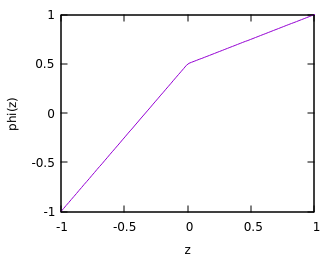
\includegraphics[width=7cm,keepaspectratio=true]{./Poisson.png}
 % Poisson.png: 0x0 pixel, 300dpi, 0.00x0.00 cm, bb=
 \caption{Illustration of the solution of the Poisson equation given by Eq.~\eqref{eq:poissonsol} for $\phi_0 = L = q = \varepsilon_0 = 1$.}
 \label{fig:poisson}
\end{figure}

In this section we will learn how to solve this equation numerically for an arbitrary charge distribution $\rho(z)$. Since it might be difficult to deal with $\delta$ distributions numerically, we shall consider, for instance, a Gaussian charge distribution $\rho(z) = q e^{-\frac{(z-z_0)^2}{2\Gamma^2}}$, where $z_0$ is the center of the distribution and $\Gamma$ is the broadening. For $z_0 = 0$ and small $\Gamma$ you should be able to reproduce the analytical solution above.


\subsection{The Sturm-Liouville problems}

In physics, many problems fall into differential equations that take the Sturm-Liouville form,

\begin{equation}
 \left\{\dfrac{d}{dx}\left[p(x) \dfrac{d}{dx}\right] + q(x)\right\}y(x) = \lambda w(x)y(x) + r(x),
 \label{eq:sturmliouville}
\end{equation}
where $p(x)$, $q(x)$, $w(x)$ and $r(x)$ are functions specified by the problem at hand, while $y(x)$ is the unknown function that we want to find. For instance, the Poisson equation in Eq.~\eqref{eq:poisson} is set by using $p(x) = 1$, $q(x) = w(x) = 0$, and $r(x) = -\rho(x)/\epsilon_0$. If $w(x) \neq 0$, $\lambda$ is the eigenvalue of the equation. We will discuss the class of eigenvalue problems later on in this Chapter, therefore, for now we shall take $w(x) = 0$. Moreover, let's assume that $p(x)$, $q(x)$ and $r(x)$ are analytical functions over the domain of interest.

Let's first present useful properties of the Sturm-Liouville equation without properly deriving them. For the derivations and more details please check specialized books on Mathematical Physics [refs] and Problem \ref{prob:sturmliouville}. Next, we use these properties to establish the Wronskian method to solve Sturm-Liouville problems.

\subsection*{The homogeneous Sturm-Liouville equation}

If $r(x) = 0$, Eq.~\eqref{eq:sturmliouville} is said homogeneous as it takes the form $\mathcal{L}y(x) = 0$, where $\mathcal{L}$ is the Sturm-Liouville operator, which is given by the terms between curly brackets, $\{\cdots\}$, in Eq.~\eqref{eq:sturmliouville}. It follows the properties:

\noindent
\textbf{(1) Principle of superposition.} Since this equation is linear, if $y_a(x)$ and $y_b(x)$ are solutions, then the linear combination $y_{c}(x) = a y_a(x) + b y_b(x)$ also satisfies $\mathcal{L}y_{c} = 0$. Here $a$ and $b$ are arbitrary constants that shall be defined by the boundary conditions, i.e. the linear combination coefficients.

\noindent
\textbf{(2) Linear independence.} Two solutions $y_a(x)$ and $y_b(x)$ are linearly independent if their Wronskian $W(x) \neq 0$ over the domain of $x$. The Wronskian of a pair of solutions $y_a(x)$ and $y_b(x)$ is $W(x) = y_a'(x) y_b(x) -y_b'(x)y_a(x)$. For the class of Sturm-Liouville homogeneous equations it is easy to show that 

\begin{equation}
 W(x) = W(x_0) \exp\left\{-\int_{x_0}^x \dfrac{p_1(x')}{p(x')}dx'\right\},
\end{equation}
where $p_1(x) = \frac{d}{dx} p(x)$, and $x_0$ belongs to the domain of $x$. Therefore, if the Wronskian $W(x_0) \neq 0$ in a specific point $x = x_0$, it will be non-zero over the whole domain.

\noindent
\textbf{(3) Uniqueness of the solution.} Since the Sturm-Liouville equation is a second-order ordinary differential equation, its solution is unique if it satisfies the ODE and two boundary (or initial) conditions. As a consequence, its most general solution can be written as a linear combination of two linearly independent solutions.

The properties above form the basis need to solve the homogeneous Sturm-Liouville problem using the Wronskian method. But before discussing this method, let's check the inhomogeneous Sturm-Liouville problem.

\subsection*{The inhomogeneous Sturm-Liouville equation}

For $r(x)\neq 0$ the Sturm-Liouville problem takes the form $\mathcal{L}y(x) = r(x)$, and is said to be inhomogeneous as it has a term independent of $y(x)$. In this case, the principle of superposition as stated above is not valid (see Problem \ref{prob:sturmliouville}). Instead, the generalized principle of superposition of inhomogeneous equations states that the most general solution can be written as

\begin{equation}
 y(x) = a y_a(x) + b y_b(x) + y_p(x),
 \label{eq:WronskianFull}
\end{equation}
where $y_a(x)$ and $y_b(x)$ are linearly independent solutions of the homogeneous equation $\mathcal{L}y_{a/b}(x) = 0$, and $y_p(x)$ is the particular solution of the inhomogeneous equation $\mathcal{L}y_p(x) = r(x)$. Here again, $a$ and $b$ are arbitrary constants to be set by the boundary conditions.

Since $y_a(x)$ and $y_b(x)$ are solutions of the homogeneous case, property \textbf{(2)} above follows and the Wronskian criteria can be used to verify or assure that $y_a(x)$ and $y_b(x)$ are linearly independent solutions. Property (3) also follows, and the solution $y(x)$ is unique if and only if it satisfies the ODE $\mathcal{L}y(x) = r(x)$ and the required boundary conditions.

\subsection{The Wronskian method}

The Wronskian method applies to both homogeneous and inhomogeneous cases of the Sturm-Liouville equation. Essentially, it provides a method to obtain a pair of linear independent solutions $y_a(x)$ and $y_b(x)$. We will state the problem for the inhomogeneous case, since the homogeneous case is simply a particular case in which $r(x) = 0$.

To guide our description let's consider Dirichlet boundary conditions, i.e. $y(x_0) = y_0$ and $y(x_1) = y_1$. Generalizations to Neumann or mixed boundary conditions will be simple enough and we leave it to the reader as an exercise. We want to solve the Sturm-Liouville equation $\mathcal{L}y(x) = r(x)$ in the domain $x_0 \leq x \leq x_1$.

\subsubsection{First step: find two linearly independent solutions of the homogeneous equation}

Our first step is to find a pair of linearly independent solutions $y_a(x)$ and $y_b(x)$ that satisfy the \textit{homogeneous} equation $\mathcal{L}y_{a/b}(x) = 0$. Accordingly to property \textbf{(2)} above, $y_a(x)$ and $y_b(x)$ will be linearly independent if their Wronskian $W(x) \neq 0$ at any point $x$. For practical purposes, we chose to analyze the Wronskian at $x = x_0$, the left end point of the domain. Namely, we want

\begin{equation}
 W(x_0) = y_a'(x_0)y_b(x_0) - y_a(x_0)y_b'(x_0) \neq 0.
\end{equation}

Notice that the final solution will be given by $y(x)$ in Eq.~\eqref{eq:WronskianFull}. Therefore the boundary conditions must apply to $y(x)$, and not to the auxiliary functions $y_a(x)$, $y_b(x)$ or $y_p(x)$. Therefore we can attribute auxiliary boundary conditions to $y_a(x)$ and $y_b(x)$ in order to assure that the condition above is satisfied and the pair $[y_a(x), y_b(x)]$ forms a set of linearly independent solutions. For instance, we may choose

\begin{align}
 y_a(x_0) &= 0, \text{  and  } y'_a(x_0) = A_1,\\
 y_b(x_0) &= A_2, \text{  and  } y'_b(x_0) = 0,
\end{align}
such that $W(x_0) = A_1 A_2$, where $A_1 \neq 0$ and $A_2 \neq 0$ are arbitrary nonzero constants.

The auxiliary boundary conditions above actually transforms the problem of finding $y_{a/b}(x)$ into a pair of independent \textbf{initial-value problems}, with the initial values for $y_a(x)$, $y_b(x)$ (and their derivatives) set above in terms of the arbitrary $A_1$ and $A_2$. We can use any initial-value problem method to obtain $y_{a/b}(x)$ satisfying the homogeneous equation $\mathcal{L}y_{a/b}(x) = 0$.

\subsubsection{Second step: find the particular solution of the inhomogeneous equation}

Now we need to find $y_p(x)$. Since this is also an auxiliary function, its boundary or initial conditions are arbitrary. Let's use $y_p(x_0) = B_1$ and $y'_p(x_0) = B_2$, where $B_1$ and $B_2$ are arbitrary constants. We can use any method of the initial-value problems to find $y_p(x)$.

\subsubsection{Third step: impose the physical boundary conditions}

In this final step we must impose the physical boundary conditions stated by our problem. Namely, we want $y(x_0) = y_0$ and $y(x_1) = y_1$. From Eq.~\eqref{eq:WronskianFull} we have

\begin{align}
 y(x_0) &= a y_a(x_0) + b y_b(x_0) + y_p(x_0) = b A_2 + B_1,\\
 y(x_1) &= a y_a(x_1) + b y_b(x_1) + y_p(x_1),
\end{align}
where $y_a(x_0) = 0$, $y_b(x_0) = A_2$, and $y_p(x_0) = B_1$ where the auxiliary initial conditions set above. The quantities $y_a(x_1)$, $y_b(x_1)$, and $y_p(x_1)$ are known from the solution of the auxiliary initial-value problems. To satisfy the boundary conditions, the coefficients $a$ and $b$ must be

\begin{align}
 b &= \dfrac{y_0-B_1}{A_2},\\
 a &= \dfrac{y_1 - b y_b(x_1) - y_p(x_1)}{y_a(x_1)}.
\end{align}

Combining these quantities, we have the all terms of Eq.~\eqref{eq:WronskianFull} to compose our final solution $y(x)$.

\subsubsection{Example: the Poisson equation via the Wronskian method}

Let's apply the Wronskian method to the Poisson equation to reproduce numerically the example of the beginning of this section; see Fig.~\ref{fig:poisson}. Let's write the Poisson equation, Eq.~\eqref{eq:poisson}, using the notation of the Sturm-Liouville problem above. It reads

\begin{equation}
 \dfrac{d^2}{dx^2} y(x) = -\rho(x).
\end{equation}
Next we use the ODE package to numerically find the auxiliary functions $y_a(x)$, $y_b(x)$ and $y_p(x)$ with appropriate initial conditions, and combine them at the end to satisfy the physical boundary condition.

The homogeneous version of the 1D Poisson's equation ($\rho(x) = 0$) is actually Laplace's equation in one dimension. Therefore it would be quite easy to find the solutions $y_a(x)$ and $y_b(x)$ of the homogeneous equation. It's simply $y_a(x) = (x-x_0)A_1$ and $y_b(x) = A_2$. However, in the numerical code below we choose to find these simple solutions numerically just to exemplify how to proceed in a more difficult scenario.

\begin{example}{Poisson via Wronskian method}
\label{ex:poissonWronskian}
\begin{minted}[mathescape,escapeinside=||]{julia}
using ODE
using PyPlot

z = linspace(-1.0, 1.0, 1000); # z axes
eps0 = 1.0; # $\varepsilon_0$

# charge density $\rho(z)$
g = 0.01; # broadening $\Gamma$
rho(z) = exp(-(z.^2)/(2*g^2))/(sqrt(2pi)*g);

# physical boundary conditions: $y_0$ and $y_1$
y0 = -1.0;
y1 = +1.0;

# find $y_a(z)$
A1 = 1.0;
ic = [0.0; A1]; # = (0, A1)
rhs(z, y) = [y[2]; 0.0];
za, ya = ode45(rhs, ic, z; points=:specified);
ya = map(k->k[1], ya);

# find $y_b(z)$
A2 = 1.0;
ic = [A2; 0.0]; # = (A2, 0)
rhs(z, y) = [y[2]; 0.0];
zb, yb = ode45(rhs, ic, z; points=:specified);
yb = map(k->k[1], yb);

# find $y_p(z)$
B1 = 0.0;
B2 = 0.0;
ic = [B1; B2]; # = (B1, B2)
rhs(z, y) = [y[2]; -rho(z)/eps0];
zp, yp = ode45(rhs, ic, z; points=:specified);
yp = map(k->k[1], yp);

# coefficients and final solution
b = (y0 - B1)/A2;
a = (y1 - b*yb[end] - yp[end])/ya[end];
y = a*ya + b*yb + yp;

plot(z, y);
\end{minted}
\end{example}

\subsection{Schroedinger equations: transmission across a barrier}

Let's consider a free electron in one dimension colliding with a general shaped barrier set by a potential $V(x)$. The dynamics of this electron is tunnel or scatter back as it collides with the barrier. Here we want to calculate the transmission $T$ and reflection $R$ probabilities.

The Hamiltonian of the system is

\begin{equation}
 H = -\dfrac{1}{2}\dfrac{\partial^2}{\partial x^2} + V(x).
\end{equation}
Here we use atomic units ($\hbar = 1$, $m=1$), and $V(x)$ is a general potential within the scattering region $0 \leq x \leq L$, and $V(x) = 0$ outside these limits.

Referring to the region $x<0$ as I, let's assume that the state of the electron is a linear combination of the injected and reflected waves,

\begin{equation}
 \psi_I(x) = e^{i k x} + r e^{-i k x},
 \label{eq:psi1}
\end{equation}
where $r$ the reflection coefficient, and $k = \sqrt{2\varepsilon}$ and $\varepsilon$ is the electron energy.

We'll refer to the region $x>L$ as III. There the electron state is composed solely by the transmitted wave,

\begin{equation}
 \psi_{III}(x) = t e^{ikx},
 \label{eq:psi3}
\end{equation}
where $t$ is the transmission coefficient.

At the central region (II), where $0 \leq x \leq L$, we need to find two linear independent solutions, $\psi_a(x)$ and $\psi_b(x)$, of the Schroedinger equation $H\psi(x) = \varepsilon\psi(x)$. I'll leave this as a Problem for the reader. These solutions can be combined in a general linear combination

\begin{equation}
 \psi_{II}(x) = a \psi_a(x) + b \psi_b(x),
 \label{eq:psi2}
\end{equation}
where $a$ and $b$ are the linear combination coefficients.

The final solution and its derivative must be continuous at the interfaces $x=0$ and $x=L$. Therefore, we impose the conditions: (i) $\psi_I(0) = \psi_{II}(0)$; (ii) $\psi'_I(0) = \psi'_{II}(0)$; (iii) $\psi_{II}(L) = \psi_{III}(L)$; (iv) $\psi'_{II}(L) = \psi'_{III}(L)$. These give us the following equation for the coefficients $a$, $b$, $r$ and $t$:

\begin{equation}
 \begin{pmatrix}
  \psi_a(0) & \psi_b(0) & -1 & 0 \\
  \psi'_a(0) & \psi'_b(0) & ik & 0 \\
  \psi_a(L) & \psi_b(L) & 0 & e^{ikL}\\
  \psi'_a(L) & \psi'_b(L) & 0 & ike^{ikL}
 \end{pmatrix}
 \begin{pmatrix}
  a \\ b \\ r \\ t
 \end{pmatrix}
 =
 \begin{pmatrix}
  1 \\ ik \\ 0 \\ 0
 \end{pmatrix}.
 \label{eq:psimatch}
\end{equation}

From the equation above one can easily extract $t$. The transmission probability is then $T = |t|^2$, and the reflection probability is $R = |r|^2$. You can check that $T+R=1$.

In Fig.~\ref{fig:transmission} we consider the transmission over a Gaussian barrier

\begin{equation}
 V(x) = e^{-\frac{1}{2}(x-x_0)^2},
\end{equation}
where $x_0 = L/2$ is the center of the barrier, and $L = 20$.

\begin{figure}[ht!]
 \centering
 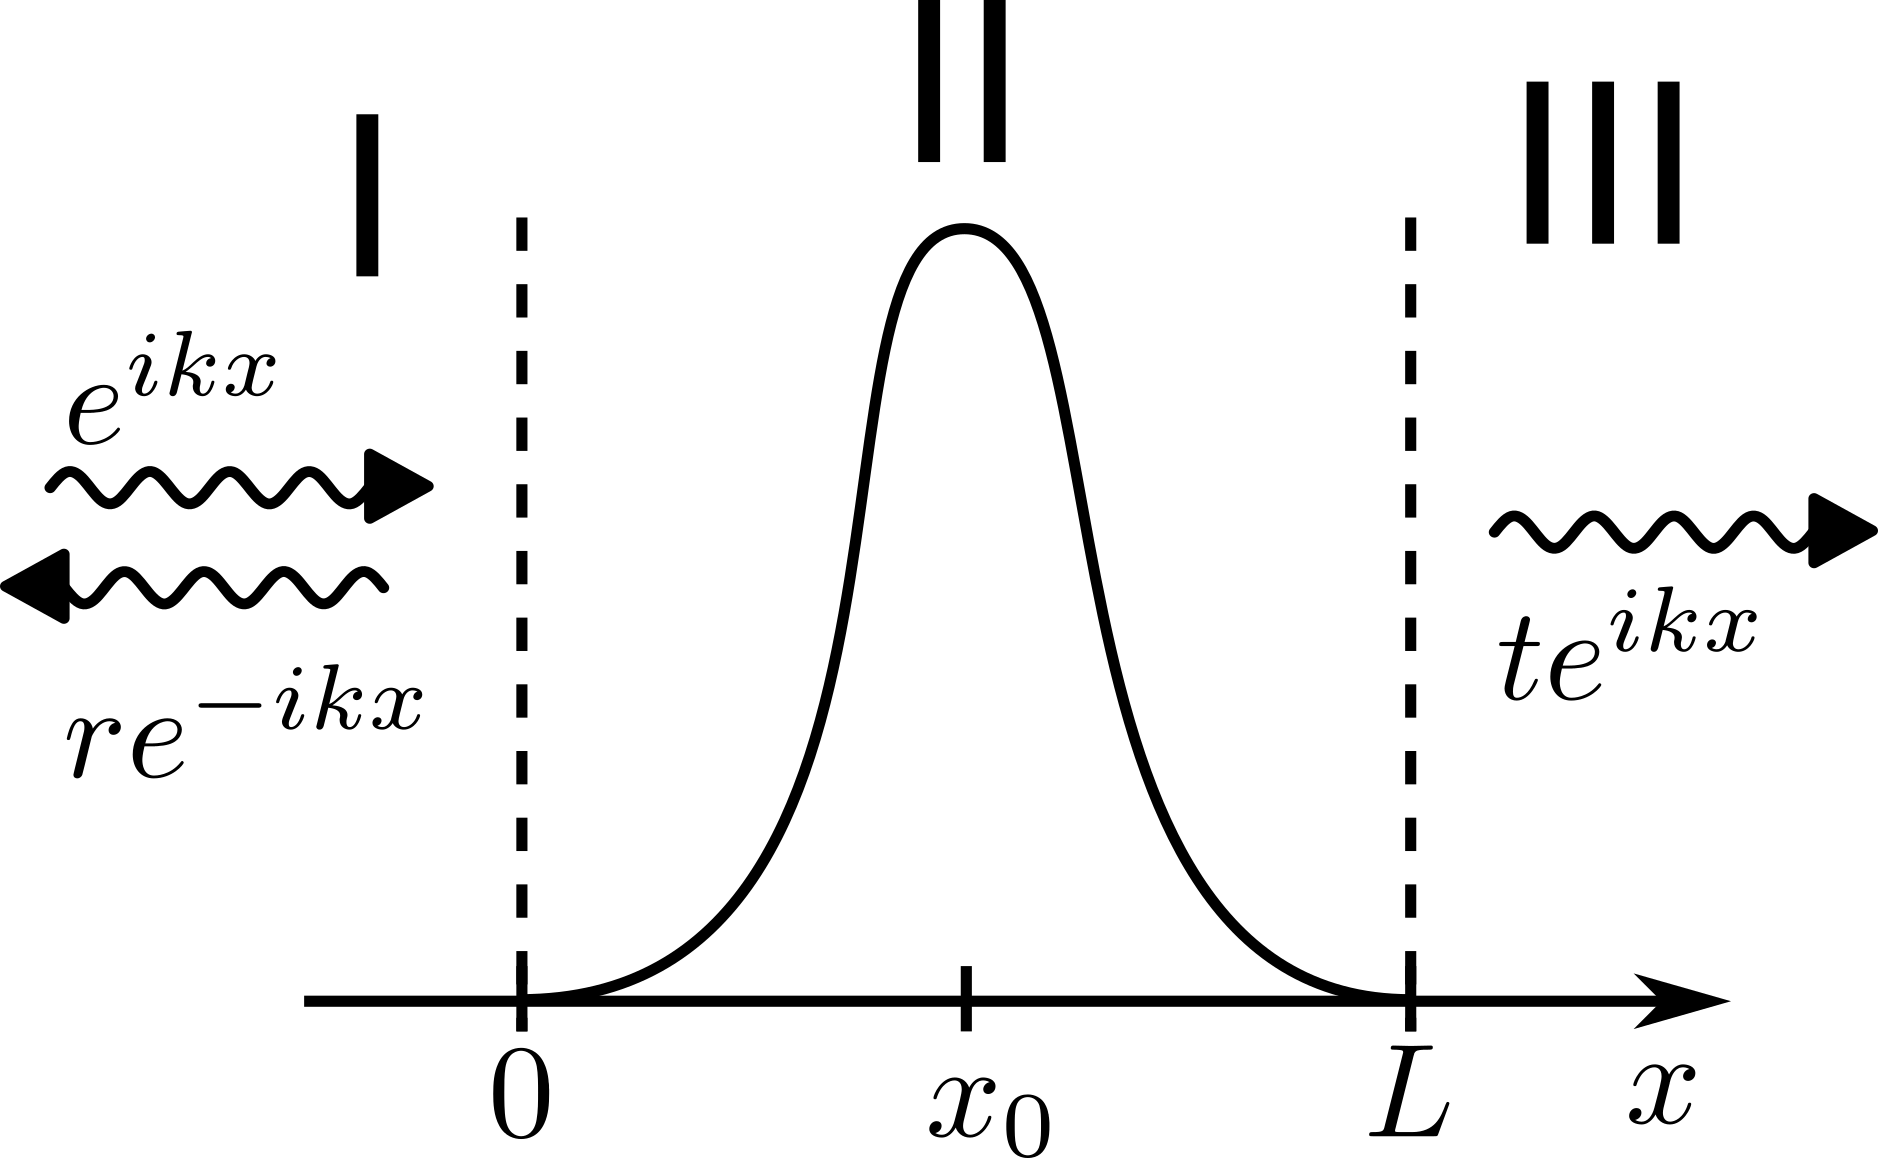
\includegraphics[width=0.45\columnwidth]{./transmissionbarrier.png}
 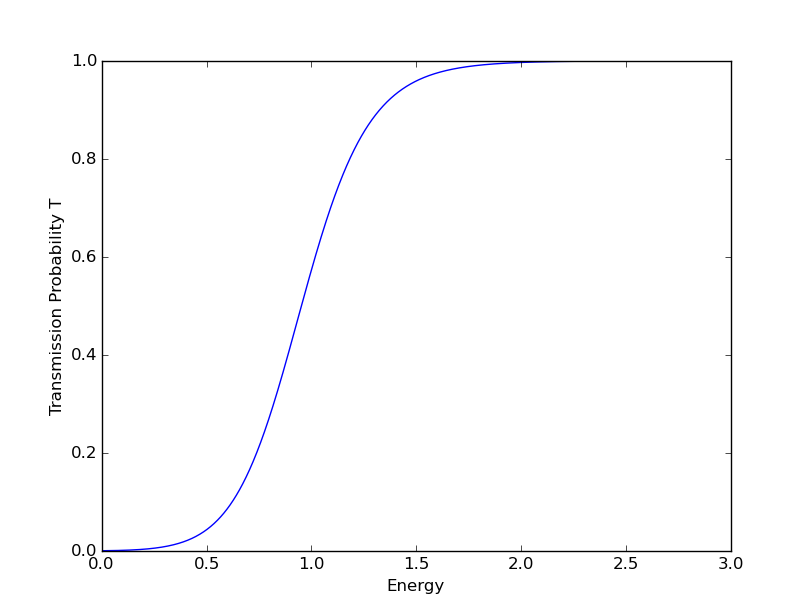
\includegraphics[width=0.45\columnwidth]{./transmission.png}
 % transmission.png: 0x0 pixel, 300dpi, 0.00x0.00 cm, bb=
 \caption{(left) Illustration of the Gaussian barrier with the injected, reflected and transmitted waves at outer regions. (right) Transmission probability $T$ as a function of the energy $\varepsilon$.}
 \label{fig:transmission}
\end{figure}


\subsection{Non-linear differential equations}

For non-linear differential equations, the properties of Sturm-Liouville operator discussed in the previous sections does not hold. Particularly, there is no superposition principle for non-linear ODEs. As a consequence, the task to solve a boundary value problem for a non-linear ODE can be quite difficult.

The non-linearity implies that a ODE with a specific set of boundary conditions may have more than one solution. This is again in direct contrast with the Sturm-Liouville case, where the uniqueness theorem (by Picard–Lindelöf) states that given the boundary or initial conditions, the ODE has only one solution.

Let's illustrate this with a very simple differential equation:

\begin{equation}
 \dfrac{d^2 y(x)}{dx^2} + |y(x)| = 0,
\end{equation}
which is non-linear due to the absolute value in the second term. Consider that the boundary conditions are $y(0) = 0$ and $y(4) = -2$.

\subsubsection{The shooting method}

One way of solving this problem is the shooting method. First, convert the second order differential equations into a pair of coupled first order differential equations. This is the same procedure used at the begging of this chapter. We know how to solve initial value problems easily. Therefore, consider the auxiliary initial conditions $y(0) = y_0$ and $y'(0) = v_0$. Clearly, it is useful to set $y_0 = 0$ to automatically satisfy our desired boundary condition. The problem is $v_0$. What is the appropriate value of $v_0$ that satisfies our boundary conditions? Namely, we want $v_0$ set such the evolution of the initial value problem yields $y(4) = -2$.

In the general there's no direct approach to find the appropriate value of $v_0$. In our example there's actually two possible values of $v_0$ that yield $y(4) = -2$. To see this, I invite the reader to write a code using the Runge-Kutta method, or Julia's ODE package to solve the initial value problem for the example above for different values of the initial condition $y'(0) = v_0$. Evolving the solution from $x=0$ to $x=4$ we can extract $y(4)$ for each value of $v_0$ and plot $y(4) \times v_0$. This is shown in Fig.~\ref{fig:shooting}.


\begin{figure}[ht!]
 \centering
 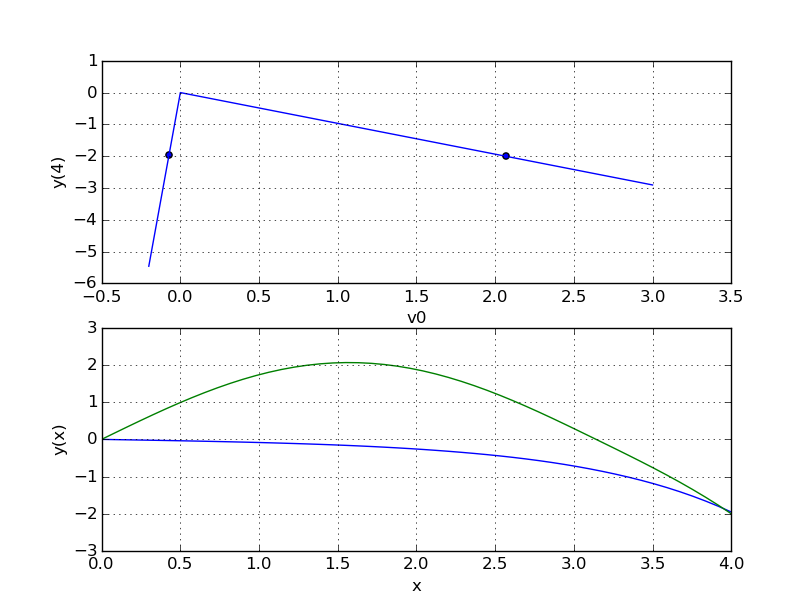
\includegraphics[width=0.70\columnwidth]{./shooting.png}
 % transmission.png: 0x0 pixel, 300dpi, 0.00x0.00 cm, bb=
 \caption{(top) Values of $y(4)$ obtained propagating the non-linear differential equation from $x=0$ to $x=4$ with the initial condition set to $y'(0) = v_0$, as a function of $v_0$. There are two values of $v_0$ that satisfy $y(4) = -2$, as indicated by the circles.
 (bottom) The two possible solutions $y(x) \times x$ for the values of $v_0$ found to satisfy the boundary conditions. }
 \label{fig:shooting}
\end{figure}

\section{The eigenvalue problem}

Here we'll consider only eigenvalue problems of linear and homogeneous differential equations. Particularly, we are only interest again in the Sturm-Liouville problems. In the Sturm-Liouville Eq.~\eqref{eq:sturmliouville}, the differential equation is an eigenvalue problem if $w(x) \neq 0$ and $r(x) = 0$. Therefore we have

\begin{equation}
 \left\{\dfrac{d}{dx}\left[p(x) \dfrac{d}{dx}\right] + q(x)\right\}y(x) = \lambda w(x)y(x),
\end{equation}
where $p(x)$, $q(x)$ and $w(x)$ are given functions set by the problem at hand, while $\lambda$ and $y(x)$ are the unknowns that we want to find. For a set of boundary conditions, this differential equation have solutions only for particular values of $\lambda$, which are called the eigenvalues. The solutions $y(x)$ associated with each particular $\lambda$ are the eigenfunctions. If we vectorize this equation using finite differences, the function $y(x)$ becomes a vector: the eigenvector.

There are many ways of solving an eigenvalue problem numerically. But let's first check two analytical cases to serve as examples where we can try our numerical approaches.

\subsection{Oscillations on a string}

A string fixed at its end points separated by a distance $\ell$ satisfy the wave equation,

\begin{equation}
 \dfrac{\partial^2 y(x,t)}{\partial x^2} - \dfrac{1}{v^2} \dfrac{\partial^2 y(x,t)}{\partial t^2} = 0,
\end{equation}
where $y(x,t)$ is the string profile as a function of space $x$ and time $t$, and $v$ is the wave velocity on the string. This is a partial differential equation, but in this chapter we are dealing with ordinary differential equations only. Since for now we are only interested in the normal modes of oscillation, we can Fourier transform the equation from time $t$ to frequency $w$, yielding

\begin{equation}
 \dfrac{\partial^2 y(x,\omega)}{\partial x^2} + \dfrac{\omega^2}{v^2} y(x,\omega) = 0.
\end{equation}
This equation takes the form of eigenvalue Sturm-Liouville problem if we set $p(x) = 1$, $q(x) = 0$, $w(x) = 1$, and $\omega^2 = v^2 \lambda$.

If the string is fixed at its end points, the boundary conditions are $y(0,t) = 0$, and $y(\ell,t) = 0$ for any $t$. Equivalently, the Fourier transformed $y(x,\omega)$ also satisfy the same boundary conditions: $y(0, \omega) = 0$ and $y(\ell, \omega) = 0$ for any $\omega$.

You have probably seen already in a theoretical physics class that the solution to this problem is

\begin{equation}
 y(x,\omega_n) = A \sin\left(\dfrac{\omega_n}{v} x\right),
\end{equation}
where $k_n = \omega_n/v$ are the quantized wave-numbers, $\omega_n = n \pi v/\ell$ are the quantized frequencies, and the integer $n$ labels the normal modes of oscillation. The amplitude $A$ depends on the initial condition, which we will not consider yet.

\subsection{Electron in a box}

An electron in a box is described by the Schroedinger equation. It's dynamics is set by the time-dependent Schroedinger equation. But similarly to the string oscillations, its normal modes are given by a static equation, the time-\textit{independent} Schroedinger equation,

\begin{equation}
 -\dfrac{1}{2}\dfrac{\partial^2}{\partial x^2} \psi(x) + V(x) \psi(x) = \varepsilon \psi(x),
 \label{eq:Schroedinger}
\end{equation}
where we use atomic units ($\hbar = 1$, $m=1$) for simplicity. Here $V(x)$ is the electrostatic potential that confines the electron, $\psi(x)$ is the wave-function and $\varepsilon$ is the energy. This is indeed a Sturm-Liouville eigenvalue problem where the eigenvalue is the energy $\varepsilon$ and the eigenfunction is the wave-function $\psi(x)$.

If the electron is trapped in a box of width $\ell$ with hard walls, such that $V(x) = 0$ for $0 < x < \ell$, and $V(x) = \infty$ outside, the wave-function must satisfy the boundary-conditions $\psi(0) = 0$ and $\psi(\ell) = 0$.

Since $V(x) = 0$ inside the box, the problem is very similar to the oscillations on a string. The solutions are

\begin{equation}
 \psi_n(x) = A \sin(k_n x),
 \label{eq:psin}
\end{equation}
where the wave-numbers $k_n = n\pi/\ell$, the eigenenergies $\varepsilon_n = \frac{1}{2}k_n^2$, and the integer $n$ labels the quantized eigenstates of the electron.

\subsection{Method of finite differences}

For simplicity let's consider the Sturm-Liouville eigenvalue problem with $p(x) = 1$ and $w(x) = 1$,

\begin{equation}
 \left\{\dfrac{d^2}{dx^2} + q(x)\right\}y(x) = \lambda y(x).
\end{equation}

We have seen in Chapter \ref{sec:matrixrepresentation} that we can represent the derivative operators as matrices. Particularly, the second derivative becomes

\begin{equation}
\dfrac{d^2}{dx^2}y(x) = 
 \begin{pmatrix}
  y''_1 \\y''_2 \\ y''_3 \\ y''_4 \\ \cdots \\ y''_i \\ \cdots \\ y''_{N-1} \\ y''_N
 \end{pmatrix}
 = \dfrac{1}{h^2}
\begin{pmatrix} 
 -2 & 1 & 0 & 0 & 0 & 0 & 0 & 0 & 0\\
 1 & -2 & 1 & 0 & 0 & 0 & 0 & 0 & 0\\
 0 & 1 & -2 & 1 & 0 & 0 & 0 & 0 & 0\\
 0 & 0 & 1 & -2 & 1 & 0 & 0 & 0 & 0\\
 0 & 0 & 0 & 1 & -2 & 1 & 0 & 0 & 0\\
 0 & 0 & 0 & 0 & 1 & -2 & 1 & 0 & 0\\
 0 & 0 & 0 & 0 & 0 & 1 & -2 & 1 & 0\\
 0 & 0 & 0 & 0 & 0 & 0 & 1 & -2 & 1\\
 0 & 0 & 0 & 0 & 0 & 0 & 0 & 1 & -2
\end{pmatrix}
\begin{pmatrix}
  y_1 \\y_2 \\ y_3 \\ y_4 \\ \cdots \\ y_i \\ \cdots \\ y_{N-1} \\ y_N
\end{pmatrix},
\end{equation}
where $y_i = y(x_i)$ and $x_i$ are the discretized coordinates.
I leave as an exercise to the reader to check that this representation is compatible with the boundary conditions $y(0) = 0$ and $y(\ell) = 0$. Here the discretization of $x$ is such that $x_0 = 0$ and $x_{N+1} = \ell$, and $h$ is the discrete step.

The $q(x)$ term is local, therefore its matrix representation is diagonal,

\begin{equation}
q(x)y(x) = 
\begin{pmatrix}
 q_1 & 0 & 0 & 0 & 0 & 0 & 0 & 0 & 0\\
 0 & q_2 & 0 & 0 & 0 & 0 & 0 & 0 & 0\\
 0 & 0 & q_3 & 0 & 0 & 0 & 0 & 0 & 0\\
 0 & 0 & 0 & q_4 & 0 & 0 & 0 & 0 & 0\\
 0 & 0 & 0 & 0 & \ddots & 0 & 0 & 0 & 0\\
 0 & 0 & 0 & 0 & 0 & q_i & 0 & 0 & 0\\
 0 & 0 & 0 & 0 & 0 & 0 & \ddots & 0 & 0\\
 0 & 0 & 0 & 0 & 0 & 0 & 0 & q_{N-1} & 0\\
 0 & 0 & 0 & 0 & 0 & 0 & 0 & 0 & q_N
\end{pmatrix}
\begin{pmatrix}
  y_1 \\y_2 \\ y_3 \\ y_4 \\ \cdots \\ y_i \\ \cdots \\ y_{N-1} \\ y_N
\end{pmatrix}.
\end{equation}
where $q_i = q(x_i)$.

With these matrix representations, the differential equation above can be put in a matrix form $H y = \lambda y$. The matrix $H$ is the sum of matrices above, $y$ is the vector composed by $y_i$, and $\lambda$ is the eigenvalue.

The most used numerical package to solve eigenvalue problems in a matrix form is Lapack\footnote{Lapack: \url{http://www.netlib.org/lapack/}}. The language Julia has this package natively implemented in the command \texttt{eig}. Try to run the next example.

\begin{example}{Eigenvalues and eigenvectors}
\label{ex:eig}
\begin{minted}[mathescape,escapeinside=||]{julia}
using PyPlot

# creates the matrix $H = -\partial_x^2$
H = 2*diagm(ones(10)) - diagm(ones(9),1) - diagm(ones(9),-1);

# calculates the eigenvalues and eigenvetors
evals, evecs = eig(H);

subplot(311)
plot(evecs[:,1]) # plot the first eigenvector

subplot(312)
plot(evecs[:,2]) # plot the second eigenvector

subplot(313)
plot(evecs[:,3]) # plot the third eigenvector

# print the first three eigenvalues
println("E1 = ", evals[1]);
println("E2 = ", evals[2]);
println("E3 = ", evals[3]);

\end{minted}
\end{example}

As you can see in the example, the \texttt{eig} command receives the matrix $H$ and returns its eigenvalues in a vector and the eigenvetors as a matrix. In this eigenvector matrix, each eigenvector is set as a column. Therefore \texttt{evecs[:,n]} returns the eigenvetor $n$.

\section{Problems}

\begin{problem}{Damped harmonic oscillator}
 \label{prob:damped}

 Implement a code to solve the damped harmonic oscillator problem,
 
 \begin{equation}
  \dfrac{d^2 x(t)}{dt^2} = -\omega_0^2 x(t) - \gamma \dfrac{dx(t)}{dt}.
 \end{equation}
 Fix $\omega_0 = 2\pi$ and solve the equation for different values of $\gamma$ to show the solutions for the three possible regimes: (i) subcritical; (ii) critical; and (iii) supercritical. You will find the exact solutions on the volume 2 of Ref.~\cite{nussenzveig2007curso}.
\end{problem}

\begin{problem}{Compare Euler and RK for the pendulum}
 \label{prob:compareEulerRK}
 
 Compare the results of Example \ref{ex:euler} and Example \ref{ex:odependulum} for small and large time steps \texttt{tau}, and for small and large oscillations (amplitude \texttt{x0}).
\end{problem}

\begin{problem}{Runge Kutta RK4}
 \label{prob:rk4}
 
 Implement your own version of the RK4 code in Julia to solve the pendulum problem or any other different equation you may prefer. Your code won't be more efficient than the adaptive code in the ODE package. However it is a good practice for you to implement the RK4 by yourself, since it is the most well known and used method for differential equations.
\end{problem}

\begin{problem}{Sturm-Liouville equation}
 \label{prob:sturmliouville}

 \textbf{Tip:} Check Moysés Nussenzveig's book, volume 2, chapter on oscillations \cite{nussenzveig2007curso}.
 
 (a) Derive the three properties listed for the homogeneous Sturm-Liouville problem: (1) principle of superposition; (2) linear independence; and (3) Uniqueness of the solution.
 
 (b) Derive the generalization of the principle of superposition for inhomogeneous equations.
  
\end{problem}

\begin{problem}{Wronskian}
 \label{prob:Wronskian}

 (a) Show that for an homogeneous Sturm-Liouville differential equation the Wronskian $W(x) = y'_a(x)y_b(x)-y_a(x)y'_b(x)$ can be written as
 
\begin{equation}
 W(x) = W(x_0) \exp\left\{-\int_{x_0}^x \dfrac{p_1(x')}{p(x')}dx'\right\},
\end{equation}

 (b) Show that if the Wronskian is nonzero over the whole domain, the solutions $y_a(x)$ and $y_b(x)$ are linearly independent. 
 
\end{problem}


\begin{problem}{Quantum transmission probability for electrons}
 
 (a) Why do we identify the positive exponentials in $\psi_I(x)$ and $\psi_{III}(x)$, Eqs.~\eqref{eq:psi1}-\eqref{eq:psi3}, as forward moving, and the negative one as a backwards motion?
 
 (b) Show that matching the continuity conditions at the interfaces $x=0$ and $x=L$ leads to Eq.~\eqref{eq:psimatch}.
 
 (c) Implement a code using the Wronskian method to obtain $\psi_a(x)$ and $\psi_b(x)$ and calculate $t$.
 
 (d) Transform the code of item (c) into a function that receives the energy $\varepsilon$ and returns the transmission $T = |t|^2$. Use this code to reproduce the transmission probability plot shown in Fig.~\ref{fig:transmission}.
 
 (e) Try now with two Gaussian barriers, and run for a thin energy grid. You will see the Fabry–Pérot resonances at the quasi-confined states of a resonant-tunneling diode.
 
\end{problem}


\begin{problem}{The Schroedinger equation and the Sturm-Liouville parameters}
 
 (a) What are the expressions for the Sturm-Liouville parameters $p(x)$, $q(x)$, $w(x)$ and $r(x)$ that represents the time-independent Schroedinger equation, Eq.~\eqref{eq:Schroedinger}? 
 
 (b) Show that the solution of electron in a box problem is given by Eq.~\eqref{eq:psin} with eigenenergies $\varepsilon_n = \frac{1}{2}(n\pi/\ell)^2$.
 
\end{problem}


\begin{problem}{Matrix representation of the derivative operator}
 
 (a) The matrix representation of the derivative operator using finite differences faces a problem at the edges. Show that this is not a problem when we consider hard wall boundary conditions: $y(0) = 0$ and $y(\ell) = 0$.
 
 (b) What changes in the matrix representation if we consider periodic boundary conditions? Namely $y(\ell) = y(0)$.
 
\end{problem}


\begin{problem}{The potential well}

  (a) Implement a code to solve the time-independent Schroedinger equation for a Gaussian potential well,
  
  \begin{equation}
   V(x) = V_0 e^{-\frac{1}{2}(x-c)^2},
  \end{equation}
  with amplitude $V_0 = -10$, centered at $c = \ell/2$, hard-wall boundary conditions $\psi(0) = \psi(\ell) = 0$, and $\ell = 10$.
  
  (b) Make a plot of the potential well and the first three eigenstates.
  
  (c) Compare the solution with a discretization of $x$ with 100 points and with 500 points. The result (eigenvalues and eigenvectors) must not change much if the implementation is correct.
 
\end{problem}








\chapter{Fourier Series and Transforms}
\vspace*{-1cm}
\begin{flushright}
\texttt{$2\pi$? Or not $2\pi$?}
\end{flushright}

The Fourier series and transform are among the most essential mathematical tools for physicists. \textcolor{red}{TO DO: Finish introduction...}

\textcolor{red}{Hereafter we assume that we are dealing with well behaved functions on their relevant domains. We shall restrict ourselves to the one-dimensinal cases. Generalizations are imediate.}

Every periodic function $f(x)$ can be expanded as a sum of trigonometric functions. If the period of the function is $\lambda$, i.e. $f(x+\lambda) = f(x)$, the \textbf{Fourier series} reads

\begin{equation}
 f(x) = \sum_{n=-\infty}^{\infty} c_n e^{-i k_n x},
 \label{eq:FourierSeries}
\end{equation}
where $k_n = 2\pi n/\lambda$, $n \in \mathbb{Z}$, and $e^{i\theta} = \cos\theta+i\sin\theta$. The coefficients $c_n$ are obtained from the orthogonality of the trigonometric functions, yielding

\begin{equation}
 c_n = \dfrac{1}{\lambda} \int_{x_0}^{x_0+\lambda} f(x) e^{i k_n x} dx.
 \label{eq:FourierSeriesInv}
\end{equation}
Here $x_0$ is arbitrary and the integral runs over one period of the function $f(x)$.

If the function $f(x)$ is not periodic, but we are interested in a finite domain $x \in [x_i,x_f]$, one can extend consider a periodic extension of $f(x)$ outside the domain, such that the Fourier series applies with the replacements $x_0 \rightarrow x_i$ and $\lambda \rightarrow x_f-x_i$. The periodic extension of $f(x)$ shall match the original function on the desired domain.

Consider now that the function $f(x)$ lives in the symmetric domain $x \in [-\frac{\lambda}{2}, \frac{\lambda}{2}]$, and we take the limit $\lambda \rightarrow \infty$. The discrete $k_n$ now become infinitesimally close, $\Delta k = k_{n+1}-k_n = \frac{2\pi}{\lambda} \rightarrow 0$, and become a continuous variable $k_n \rightarrow k$. Converting the sum in Eq.~\eqref{eq:FourierSeries} into an integral with $\sum_n \rightarrow \frac{\lambda}{2\pi}\int dk$, and replacing $c_n \rightarrow (\sqrt{2\pi}/\lambda)\tilde{f}(k)$, the Fourier series, Eq.~\eqref{eq:FourierSeries}, becomes

\begin{align}
 f(x) &= \dfrac{1}{\sqrt{2\pi}} \int_{-\infty}^{\infty} \tilde{f}(k) e^{-i k x} dk,\\
 \tilde{f}(k) &= \dfrac{1}{\sqrt{2\pi}} \int_{-\infty}^{\infty} f(x) e^{i k x} dx,
\end{align}
where $\tilde{f}(k) = F[f(x)]$ is the Fourier transform of $f(x)$, and reciprocally, $f(x) = F^{-1}[\tilde{f}(k)]$ is the inverse Fourier transform of $\tilde{f}(k)$.

The next example shows the Fourier series. Play with the function and parameters.

\begin{example}{Fourier Series}
\label{ex:FourierSeries}
\begin{minted}[escapeinside=||,mathescape]{julia}
using PyPlot

x = linspace(0.0, 30.0, 300); # domain
f(x) = sin(x)./x; # example function

lambda = x[end]-x[1]; # period
k(n) = 2pi*n/lambda; # wave number

# define a function to caculate the coefficients $c_n$
c(n) = quadgk(x->f(x)*exp(1im*k(n)*x), x[1], x[end])[1]/lambda;

N = 10; # the sum will be $\displaystyle \sum_{n=-N}^N$
Ni = -N:N; # array of values of $n$
Ci = [c(n) for n=Ni]; # calculate the coefficients and store in an array

# combine the arrays to recover the approximate function
fa=sum(i-> Ci[i]*exp(-1im*k(Ni[i])*x), 1:(2*N+1))

clf(); # the plot is shown in $\text{Fig. \ref{fig:FourierSeries}}$
subplot2grid((2,2),(0,0),colspan=2)
plot(x,f(x)); # plot the original function
plot(x, real(fa)) # and the approximated one
xlabel(L"$ x $");
ylabel(L"$ f(x) $");

subplot2grid((2,2),(1,0))
vlines(Ni, 0, real(Ci)); # real part of $c_n$
scatter(Ni, real(Ci));
xlabel(L"$ n $")
ylabel(L"$ Re\{c_n\} $")

subplot2grid((2,2),(1,1))
vlines(Ni, 0, imag(Ci)); # imaginary part of $c_n$
scatter(Ni, imag(Ci));
xlabel(L"$ n $")
ylabel(L"$ Im\{c_n\} $")

tight_layout();
\end{minted}
\end{example}

\begin{figure}[ht!]
 \centering
 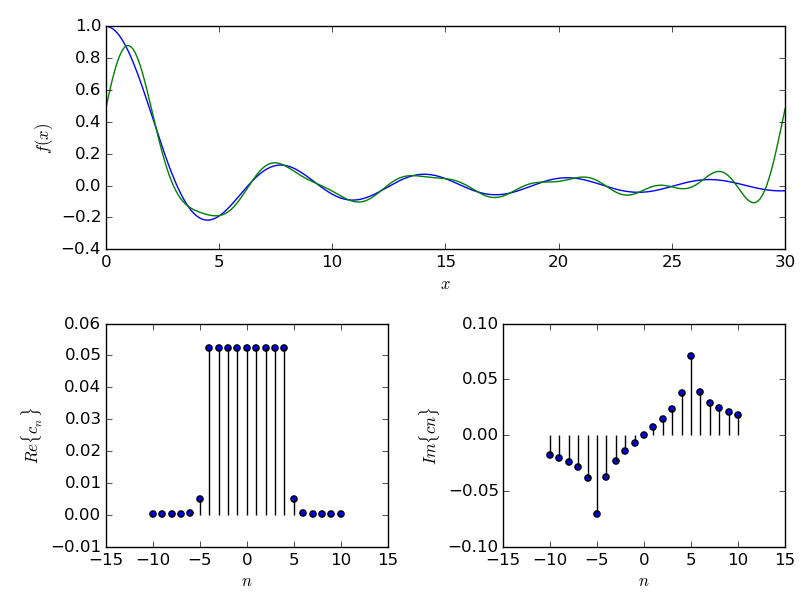
\includegraphics[width=14cm,keepaspectratio=true]{./FourierSeries.png}
 \caption{Output of Example \ref{ex:FourierSeries}.}
 \label{fig:FourierSeries}
\end{figure}

Typically, when we work with a function $f(x)$, where $x$ is a space coordinate, the Fourier transform is set in terms of the wave-number $k$ as above. If our signal is a function of time, i.e. $f(t)$, the Fourier transform is usually set in terms of the angular frequency $\omega$ as $\tilde{f}(\omega) = F[f(t)]$. 

\section{General properties of the Fourier transform}

There are many important properties of the Fourier transform that can be applied to solve physics problems. Here I'll list (without demonstrations) a few properties that will be useful for us in this Chapter. 

\subsubsection*{Linearity}

Let $f(x) = A g(x) + B h(x)$, the Fourier transform of $f(x)$ is $\tilde{f}(k) = A \tilde{g}(k) + B \tilde{h}(k)$.

\subsubsection*{Translation}

For a constant shift $x_0$ in $f(x) = g(x-x_0)$, we get $\tilde{f}(k) = e^{-i x_0 k}\tilde{g}(k)$.
Equivalently, a phase set by $k_0$ as $f(x) = e^{i k_0 x} g(x)$ leads to a Fourier transform shifted in the reciprocal space $\tilde{f}(k) = g(k-k_0)$.

\subsubsection*{Scaling}

For a real number $A$ in $f(x) = g(Ax)$, the Fourier transform scales as $\tilde{f}(k) = \frac{1}{|A|}\tilde{g}(k/A)$.

\subsubsection*{Derivatives}

Let $f_n(x) = \frac{d^n}{dx^n}g(x)$ denote the $n$-th derivative of $g(x)$, the transform is $\tilde{f}_n(k) = (ik)^n\tilde{g}(k)$.

\noindent
Equivalently, for $f(x) = x^n g(x)$, the transform is $\tilde{f}(k) = i^n \frac{d^n}{dk^n}\tilde{g}(k)$.

\subsubsection*{Convolution}

The convolution of the functions $g(x)$ and $h(x)$ is

\begin{equation}
 f(x) = (g\ast h)(x) = \int_{-\infty}^{\infty}g(x')h(x-x')dx'.
\end{equation}

The Fourier transform of a convolution is $\tilde{f}(k) = \sqrt{2\pi}\tilde{g}(k)\tilde{h}(k)$, which is simply the product of Fourier transformed functions. Conversely, if the function is the product of $g(x)$ and $h(x)$, i.e. $f(x) = g(x)h(x)$, the Fourier transform is $\tilde{f}(k) = (\tilde{g}\ast\tilde{h})/\sqrt{2\pi}$.


\section{Numerical implementations}

\subsection{Discrete Fourier Transform (DFT)}

The Discrete Fourier Transform is equivalent to the Fourier series applied on a discrete $x$ lattice. It can be obtained from Eqs.~\eqref{eq:FourierSeries}-\eqref{eq:FourierSeriesInv} for $x_0 = 0$, $dx = \lambda/N$, $x \rightarrow x_n = n\lambda/N$, and converting the integral in Eq.~\eqref{eq:FourierSeriesInv} into a sum.

Let $f$ be an array with $N$ elements representing the function $f(x)$. The Fourier transform $\tilde{f}(k) = F[f(x)]$ is represented by an array $\tilde{f}$ whose elements are

\begin{equation}
 \tilde{f}_m = \sum_{n=1}^N f_n \exp\left[-i \dfrac{2\pi(n-1)(m-1)}{N}\right].
\end{equation}

Conversely, given a vector $\tilde{f}$ representing a function $\tilde{f}(k)$ in k-space, the inverse Fourier transform $f(x) = F[\tilde{f}(k)]$ is represented by the array $f$ with elements

\begin{equation}
  f_n = \dfrac{1}{N} \sum_{m=1}^N \tilde{f}_m \exp\left[+i \dfrac{2\pi(m-1)(n-1)}{N}\right].
\end{equation}

Since we have to calculate all elements to compose the full array $\tilde{f}$ or $f$, the DFT or the inverse DFT takes $N^2$ operations. In contrast, the \texttt{Fast Fourier Transform} (FFT) algorithm takes $N\log_2 N$ operations, which is much smaller than $N^2$ for large $N$.

\subsection{Fast Fourier Transform (FFT)}

\red{(TO DO)} Here I'll follow the Radix-2 code of Cooley-Tukey: \url{https://en.wikipedia.org/wiki/Cooley%E2%80%93Tukey_FFT_algorithm}


\subsection{Julia's native FFT}

Julia comes with a native implementation of FFT via the efficient FFTW library\footnote{FFTW: \url{http://www.fftw.org/}}. We have implicitly used the FFT before when using the command \texttt{conv} to perform convolutions. The main commands to remember are \texttt{fft}, \texttt{ifft}, \texttt{fftshift}, and \texttt{ifftshift}.

These functions act on arrays. Therefore, hereafter consider a discrete domain (\texttt{linspace)} $x$ with spacing $\Delta x$ and the array $f(x) \rightarrow f$ set on this domain. 

\begin{figure}[ht!]
 \centering
 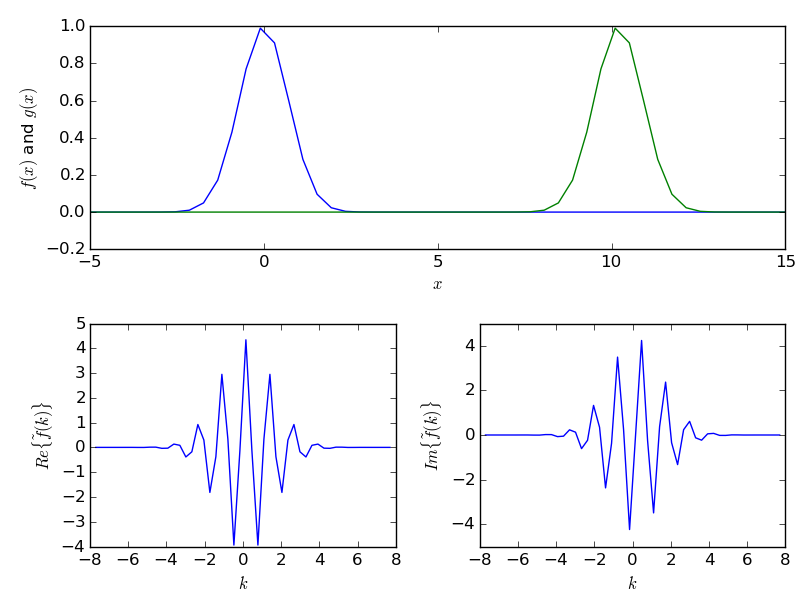
\includegraphics[width=14cm,keepaspectratio=true]{./FTShift.png}
 \caption{Output of Example \ref{ex:FTShift}.}
 \label{fig:FTShift}
\end{figure}

First, the command \texttt{fft} acts on an array $f$ and returns its Fourier transform $\tilde{f}$. Reciprocally, the command \texttt{ifft} acts on the array $\tilde{f}$ and returns its inverse Fourier transform $f$.

Notice that the array $f$ represents the function $f(x)$ over the discrete domain set by the array $x$. Conversely, the array $\tilde{f}$ represents the Fourier transformed function $\tilde{f}(k)$. The FFT implementation defines the domain of reciprocal space as $k \in [0, \frac{2\pi}{\Delta x})$. However, due to the periodicity of the Fourier transforms, the region $\frac{\pi}{\Delta x} \leq k < \frac{2\pi}{\Delta x}$ is actually equivalent to the region $-\frac{\pi}{\Delta x} \leq k < 0$. Typically, it is more interesting to work on the reciprocal space in the symmetric domain $k \in [-\frac{\pi}{\Delta x}, \frac{\pi}{\Delta x})$. 

One can use the commands \texttt{fftshift} and \texttt{ifftshift} to switch between these choices of domains above. The \texttt{fftshit} converts the domain from $k \in [0, \frac{2\pi}{\Delta x})$ into $k \in [-\frac{\pi}{\Delta x}, \frac{\pi}{\Delta x})$, while \texttt{ifftshift} performs the inverse operation.

The next example uses the translation property of the Fourier transform to shift a function by $x_0$. Check also Problem \ref{prob:FFTdiff}.

\begin{example}{Fourier transform using the FFT}
\label{ex:FTShift}
\begin{minted}[escapeinside=||,mathescape]{julia}
using PyPlot

n = 50; # using a small number of points for better visualization
x = linspace(-5.0, 15.0, n); # $x$ domain
dx = x[2]-x[1]; # spacing $\Delta x$
k = linspace(-pi/dx, pi/dx, n); # $k$ domain (symmetric)

# function in x-space
f = exp(-x.^2); # example function

# function in k-space
# and using fftshift to put ft in the symmetric domain
ft = fftshift(fft(f)); 

x0 = 10; # let's shift the function
gk = ft.* exp(-1im*x0*k); # see the Fourier transform properties
# goes back to the $[0,\frac{2pi}{dx})$ k-domain and apply ifft
g = ifft(ifftshift(gk)); 
# $g(x) = F^{-1}\big[ e^{-ix_0k}\tilde{f}(k)\big]$

clf(); # the plot is shown in $\text{Fig. \ref{fig:FTShift}}$
subplot2grid((2,2),(0,0),colspan=2)
plot(x,f); # plot the original function
plot(x, real(g)) # and shifted one
xlabel(L"$x$");
ylabel(L"$f(x)$ and $g(x)$")

# plot the real part of the Fourier transform
# shifting to the symmetric $k$-domain
subplot2grid((2,2),(1,0))
plot(k, real(ft));
xlabel(L"$k$")
ylabel(L"$Re\{\tilde{f}(k)\} $")

# plot the imaginary part of the Fourier transform
# shifting to the symmetric $k$-domain
subplot2grid((2,2),(1,1))
plot(k, imag(ft));
xlabel(L"$k$")
ylabel(L"$Im\{\tilde{f}(k)\} $")

tight_layout();
\end{minted}
\end{example}

\section{Applications of the FFT}

\subsection{Spectral analysis and frequency filters}

Let $\tilde{f}(\omega) = F[f(t)]$ be the Fourier transform of $f(t)$. The power spectrum of $f(t)$ is $S(\omega) = |\tilde{f}(\omega)|^2$. The plot of $S(\omega)$ \textit{vs} $\omega$ shows us which components (frequencies $\omega$) of the Fourier transform contribute to the signal $f(t)$. The power spectrum characterizes the color of a light beam, and the timbre of a musical instrument.

If our signal is simply $f(t) = A \sin(\omega_0 t)$, its Fourier transform is 

\begin{equation}
\tilde{f}(\omega) = i A \sqrt{\dfrac{\pi}{2}}\Big[\delta(\omega-\omega_0)-\delta(\omega+\omega_0)\Big],
\end{equation}
and the power spectrum will show two $\delta$-peaks at $\omega = \pm \omega_0$. This is the expected solution of the simple pendulum in the harmonic regime. Check Problem \ref{prob:FFTpendulum}.

\subsubsection{Noise and frequency filters}

What if our signal was noisy? There are many types of noise depending on their source\footnote{\href{https://en.wikipedia.org/wiki/Colors\_of\_noise}{The colors of noise (Wikipedia)}}. Musical instruments may suffer from high frequency noises due to electronic systems, bad cables, etc. The type of noise is defined by its power spectrum. For instance, a \textit{white noise} shows a constant power spectrum will all frequencies contributing equally. Hence the name \textit{white noise} as a reference to white light. The power spectrum of a \textit{pink noise} decays with $1/\omega$ and appears in most natural phenomena. The types of noise got their names as colors due to the initial analogy of white noise and white light.

In the next example, let's artificially generate and eliminate a white noise. The result is shown if Fig.~\ref{fig:whitenoise}. The white noise in this example have a power spectrum $S(\omega) \approx 10$, and two signal peaks show at $\omega = \pm 2\pi$. To filter the white noise we simply collect only the fft components that are above the white noise power spectrum.

\begin{example}{White noise}
\label{ex:whitenoise}
\begin{minted}[escapeinside=||,mathescape]{julia}
using PyPlot

N=300000; # generate signal with large number of points
t=linspace(0, 30, N); # time domain
dt=t[2]-t[1];
w=linspace(0, 2pi/dt, N); # frequency domain

w0 = 2pi; # original frequency of the signal
# signal + random fluctations:
f=(1+0.5*randn(N)).*sin((1+0.001*randn(N)).*w0.*t); 

g = fft(f); # fft of the signal
s = log(abs2(g)); # power spectrum of the signal

g2 = g.*(s .> 15); # filters the spectrum above the white noise (~10)
s2 = log(1e-10+abs2(g2)); # spectrum of the filtered signal
f2 = ifft(g2); # recovers filtered signal with inverse FFT

clf();
subplot(211)
# first half shows original signal with noise
# second half shows filtered signal, now clean
n2 = Int(N/2);
plot(t[1:n2], f[1:n2])
plot(t[n2:end], f2[n2:end]);
xlabel(L"t")
ylabel(L"f(t)");

subplot(212)
# plot the power spectra
plot(w-pi/dt, fftshift(s));
plot(w-pi/dt, fftshift(s2));
xlim([-3w0, 3w0]);
xlabel(L"\omega")
ylabel(L"\logS(\omega)");

tight_layout();
\end{minted}
\end{example}

\begin{figure}[ht!]
 \centering
 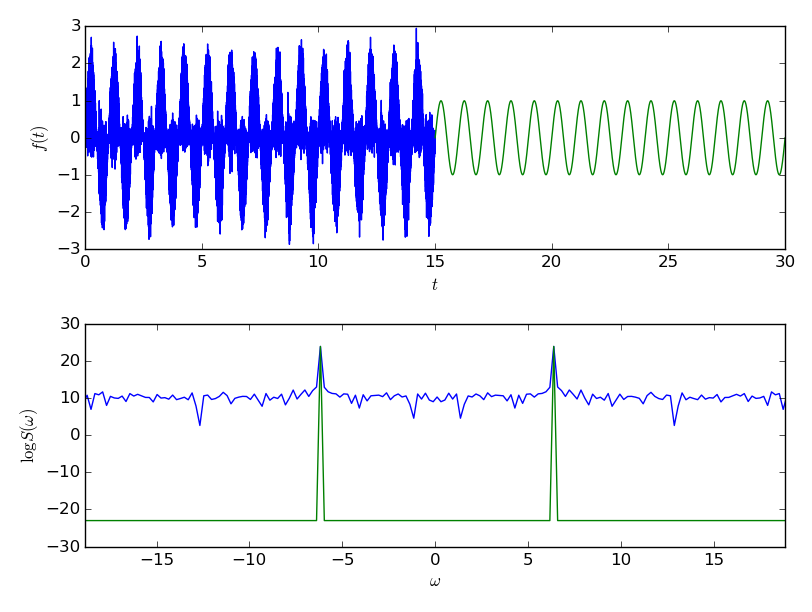
\includegraphics[width=14cm,keepaspectratio=true]{./whitenoise.png}
 \caption{Output of Example \ref{ex:whitenoise}.}
 \label{fig:whitenoise}
\end{figure}

In practice, each noise color requires a different method to be eliminated. Typical cases are the high-pass and low-pass filters, that apply frequency cuts to allow only high and low frequencies, respectively. 

\subsection{Solving ordinary and partial differential equations}
\label{sec:fourierPDE}

There are many different approaches to solve partial differential equations (PDE), which we will discuss in Chapter \ref{chap:PDE}. For now, we shall discuss only the a method using the Fourier transform. As paradigmatic examples, we will use the diffusion equation for the homogeneous case, and the Schrödinger equation for the inhomogeneous case. However, keep in mind that the method used in the Schrödinger equation is also valid for an inhomogeneous diffusion equation.

\subsubsection{Diffusion equation}

Let's consider the homogeneous diffusion equation in one dimension,

\begin{equation}
 \dfrac{\partial}{\partial t}u(x,t) - D \dfrac{\partial^2}{\partial x^2}u(x,t) + v \dfrac{\partial}{\partial x} u(x,t) = 0,
\end{equation}
where $D$ is the diffusion coefficient, $v$ is the drift velocity and $u(x,t)$ is density of the diffusing material (mass, temperature, ...).

In this very simple homogeneous case, the diffusion equation has an analytical solution. For an initial condition $u(x,0) = \delta(x)$,

\begin{equation}
 u(x,t) = \dfrac{1}{2\sqrt{\pi D t}}\exp \left[-\dfrac{(x-vt)^2}{4 D t}\right],
\end{equation}
which is a Gaussian packet with a center that moves as $x = vt$, and broadens with time.

To find this solution, we first take the Fourier transform $x \rightarrow k$ of the diffusion equation,

\begin{equation}
 \dfrac{\partial}{\partial t}\tilde{u}(k,t) + D k^2 \tilde{u}(k,t) + i v k \tilde{u}(k,t) = 0.
\end{equation}
It is easy to show that the solution in $k$-space is $\tilde{u}(k,t) = e^{(-ivk-dk^2)t}\tilde{u}(k,0)$, where $\tilde{u}(k,0)$ is the Fourier transform of the initial condition $u(x,0)$. If the initial condition is $u(x,0) = \delta(x)$, then $\tilde{u}(k,0) = 1/\sqrt{2\pi}$. The inverse Fourier transform can be easily calculated analytically to obtain the solution $u(x,t)$ above.

In this simple case we don't really need any numerical calculation. However, you could eventually face a more general diffusion equation (inhomogeneous, vectorial, coupled, ...) for which numerical methods will be necessary. Therefore, let's illustrate the numerical method assuming that you are able to obtain the solution in $k$-space $\tilde{u}(k,t)$ analytically, but you are not able to calculate the Fourier transform of the initial condition  $\tilde{u}(k,0) =  F[u(x,0)]$ and the inverse Fourier transform to recover $u(x,t) = F^{-1}[\tilde{u}(k,t)]$. The next example solves this problem.

\begin{example}{Diffusion equation}
\label{ex:diffusion}
\begin{minted}[escapeinside=||,mathescape]{julia}
using PyPlot

D = 1; # diffusion coefficient
v = 1; # drift velocity

N = 100; # number of points
L = -10; 
x = linspace(-L, L, N); # x domain
dx = x[2]-x[1]; # x step
k = linspace(-pi/dx, pi/dx, N); # k domain (symmetric)

ux0 = exp(-x.^2); # initial condition $u(x,0)$
uk0 = fftshift(fft(ux0)); # initial condition in k-space $\tilde{u}(k,0)$

# analytical solution in k-space written with the numerical k vector
ukt(t) = exp((-1im*v*k-D*k.^2)*t).*uk0;

# the solution $u(x,t)$ as a function that uses the inverse FFT
uxt(t) = ifft(ifftshift(ukt(t)));

# plot the resuts for different times $t = 0, 1, 2, 3$
clf();
plot(x, ux0);
plot(x, uxt(1));
plot(x, uxt(2));
plot(x, uxt(3));
xlabel(L"$x$");
ylabel(L"$u(x,t)$"];
\end{minted}
\end{example}

\subsubsection{Quantum operators in k-space, the split-step method}

\red{Trying to find an easy way to prove the $\mathcal{O}(\tau^3)$}

Let $H(x,p,t) = T(p,t) + V(x,t)$ be a general Hamiltonian that can be written as a sum of two terms, where the first, $T(p,t)$, is a function of the momentum operator $p = -i\hbar\partial_x$ and the time $t$, while the second, $V(x,t)$, is a function of the position $x$ and time $t$. In general the commutator $[T,V] \neq 0$. We want to solve the time-dependent Schrödinger equation

\begin{equation}
 i\hbar \dfrac{\partial}{\partial t} \psi(x,t) = H(x,p,t)\psi(x,t). 
\end{equation}

For a small time step $\tau$, an approximate numerical solution can be computed as

\begin{equation}
 \psi(x, t+\tau) \approx e^{-i\frac{V\tau}{2\hbar}}  e^{-i\frac{T\tau}{\hbar}}  e^{-i\frac{V\tau}{2\hbar}}\psi(x,t).
\end{equation}
Here we start with half of a time step, $\tau/2$ using V, followed by a full time step $\tau$ using $T$, and another $\tau/2$ to complete the evolution from $t$ to $t+\tau$. This spitting of the operators generates an error of order $\mathcal{O}(\tau^3)$.

More interestingly, this approach can be extremely efficient if we notice that $T$ is a function of momentum $p$, and, therefore, can be better represented in Fourier space (see the derivative property of the Fourier transform). The trick is to carry all operations using $V$ in coordinates space, while those involving $T$ are done in $k$-space. In terms of Fourier transforms, the evolution reads

\begin{equation}
 \psi(x, t+\tau) \approx \exp\left(-i\dfrac{V\tau}{2\hbar}\right) F^{-1}\Big[ \exp\left(-i\dfrac{\tilde{T}\tau}{\hbar}\right)  F\Big[\exp\left(-i\dfrac{V\tau}{2\hbar}\right)  \psi(x,t)\Big]\Big],
\end{equation}
where $\tilde{T} \equiv \tilde{T}(k,t)$ is the Fourier transform $p \rightarrow \hbar k$ of the $T(p,t)$ operator.

Notice that $V(x,t)$ becomes a diagonal matrix when we discretize $x$, but $T(p,t)$ is non-diagonal, as it contains derivatives in the momentum operator. However, in k-space, $\tilde{T}(k,t)$ is diagonal. Therefore, using the Fourier transform as in the equations above, all exponentials will be defined in terms of diagonal matrices, which is easy to calculate. In fact, calculating the exponential of a general matrix is much less efficient than the FFT. Hence the high efficiency of the split-step method. The next example illustrates the difference between the coordinate- and k-space calculations of $\phi = \exp\left(-i\frac{T\tau}{\hbar}\right)\phi_0$, where $T = -\frac{1}{2}p^2$.



\section{Problems}

\begin{problem}{Discrete Fourier Transform}
  \label{prob:DFT}

  Implement your own version of the Discrete Fourier Transform (DFT) in Julia and compare the results with Example \ref{ex:FTShift}. Your implementation will not be efficient and you shall use Julia's native \texttt{fft} function always. However, implementing the DFT will help you learn more about coding.

\end{problem}

\begin{problem}{Derivatives with the FFT package}
  \label{prob:FFTdiff}
  
  Check again Example \ref{ex:FTShift} and adapt it to use the derivative property of the Fourier transforms to calculate the first, second, and third derivatives of a function $f(x)$ set on a discrete domain. Choose a simple function $f(x)$, so that you can find its derivatives analytically and compare with the numeric results.  
 
\end{problem}

\begin{problem}{Pendulum: small vs large amplitudes}
 \label{prob:FFTpendulum}
 
 In the previous chapter, you have written a code to solve the differential equation of a pendulum,
 
 \begin{equation}
   \dfrac{d^2}{dt^2} x(t) = -\omega_0^2 \sin[x(t)] -\gamma v_x(t).
  \end{equation}
 
 For now, let's neglect the damping term, $\gamma = 0$. Consider $\omega_0 = 2\pi$ and the initial conditions $x(0) = x_0$, and $v(0) = 0$. Prepare your code to run over $0 \leq t \leq 100$.
 
 (a) Find $x(t)$ for small amplitudes set by $x_0 = 0.01\pi$ and use the \texttt{fft} command to obtain $\tilde{x}(\omega)$. Plot the spectral function $S(\omega) = |\tilde{x}(\omega)|^2$ for $-2\omega_0 \leq \omega \leq 2\omega_0$.

 (b) Do the same for large amplitudes set by $x_0 = 0.99\pi$.
 
 (c) Discuss the differences between the power spectra of cases (a) and (b).
 
\end{problem}


\begin{problem}{Pendulum: large amplitudes and damping}
 \label{prob:FFTpendulum2}
 
 Consider the same equation an parameters from the previous problem. But now let's start with a large amplitude $x_0 = 0.99\pi$, and a finite damping $\gamma = 0.001$. Solve the differential equation for $0 \leq t \leq 6000$ with a large number of points ($\sim 10^5$). As a function of $t$ you shall see the oscillations loosing amplitude due to the damping.
 
 (a) Plot the spectral function $S(\omega)$ using only the numerical data of $x(t)$ for small $t$, say in a window $0 \leq t \leq 500$.
 
 (b) Plot $S(\omega)$ for the data at large $t$, say in a window $5500 \leq t \leq 6000$.
 
 (c) Explain the difference between the spectral functions.
 
\end{problem}


\begin{problem}{Driven pendulum}
  \label{prob:drivenpendulum}

  Let's analyze the power spectrum of a driven pendulum\cite{pang2006introduction}. Consider a driven pendulum set by 
  
  \begin{equation}
   \dfrac{d^2}{dt^2} x(t) = -\omega_0^2 \sin[x(t)] -\gamma v_x(t) + f_0\cos(\omega_1 t).
  \end{equation}

  (a) Solve this differential equation for $x(0) = 0$, $v_x(0) = 2$, and $0 < t < 3000$, using the parameters $\omega_0 = 1$, $\omega_1 = 2/3$, $\gamma = 1/2$, and $f_0 = 0.9$.
  
  (b) Now try it with the same parameters, except for $f_0 = 1.15$.
  
  (c) The power spectrum is $S(\omega) = |\tilde{x}(\omega)|^2$, where $\tilde{x}(\omega)$ is the Fourier transform ($t \rightarrow \omega$) of $x(t)$. Compare the power spectra of cases (a) and (b). The first is periodic, and will show narrow peaks at the motion frequencies. The second is chaotic, almost all frequencies contribute and the power spectrum is fractal.
  
\end{problem}





% ***************************************
\chapter{Statistics \textcolor{red}{(TO DO)}}
\vspace*{-1cm}
\begin{flushright}
\texttt{What are the odds of having a silly quote here?}
\end{flushright}

\section{Random numbers}
\section{Random walk and diffusion}
\section{The Monte Carlo method}
% ***************************************


% ***************************************
\chapter{Partial Differential Equations \textcolor{red}{(TO DO)}}
\label{chap:PDE}
% \vspace*{-1cm}
% \begin{flushright}
% \texttt{What are the odds of having a silly quote here?}
% \end{flushright}

\section{Separation of variables}
\section{Discretization in multiple dimensions}
\section{Iterative methods, relaxation}
\section{Fourier transform (see \S\ref{sec:fourierPDE})}

% ***************************************

\chapter{Plotting  \textcolor{red}{(not finished)}}
\vspace*{-1cm}
\begin{flushright}
\texttt{... is worth a thousand words}
\end{flushright}

\lettrine[nindent=0.35em,lhang=0.40,loversize=0.3]{J}{ulia} has a few interesting packages for plotting:

\begin{itemize}
 \item \texttt{PyPlot}\footnote{PyPlot: \url{https://github.com/stevengj/PyPlot.jl}}: provides an interface to Python's MatPlotLib;
 \item \texttt{Gaston}\footnote{Gaston: \url{https://github.com/mbaz/Gaston.jl}}: provides a \texttt{gnuplot} interface to Julia;
 \item \texttt{Gadfly}\footnote{Gadfly: \url{http://dcjones.github.io/Gadfly.jl/}}: ``The Grammar of Graphics'';
 \item \texttt{Winston}\footnote{Winston: \url{https://github.com/nolta/Winston.jl}}: brings the MATLAB syntax to Julia plots.
\end{itemize}

Here we will discuss \texttt{PyPlot} to take advantage of its extensive documentation and large number of users, making it easy to find examples online. 
% Additionally we present \texttt{gnuplot}, which is a traditional and powerful tool for scientific plotting. \texttt{Gnuplot} can be used with Julia via the \texttt{Gaston} package, but we will not cover this package here.

\section{PyPlot}
\label{sec:PyPlot}

\subsection{Installing PyPlot}

To install \texttt{PyPlot}, first you need Python and Matplotlib. If you use Ubuntu Linux, run

\begin{minted}{bash}
 $ sudo apt-get update
 $ sudo apt-get install python python-matplotlib
\end{minted}

Now you can install PyPlot. Start Julia and run: \mintinline[escapeinside=||]{julia}{|\julia| Pkg.add("PyPlot")}.

\subsection{Using PyPlot}

To use \texttt{PyPlot}, first you have to initialize it by calling: \mintinline[escapeinside=||]{julia}{|\julia| using PyPlot}. 

\begin{example}{Using PyPlot}
\begin{minted}{julia}
using PyPlot
x = linspace(-3pi,3pi,200);
plot(x,  sin(x)./x, color="red", linewidth=2.0, linestyle="-");
plot(x, -sin(x)./x, color="blue", linewidth=2.0, linestyle="--");
xlabel("x");
ylabel("f(x)");
\end{minted}
\end{example}

Since the \texttt{PyPlot} package is an interface to Python's Matplotlib, one may use its extensive documentation\footnote{Matplotlib's documentation: \url{http://matplotlib.org/}}.


\subsection{Most useful features and examples}

\subsubsection{Calling non-ported functions from Matplotlib}

PyPlot's documentation says that only the documented Python's \texttt{matplotlib.pyplot} API is exported to Julia. Nonetheless, other functions from Python's \texttt{PyPlot} can be accessed as

\begin{center}
 \texttt{matplotlib.pyplot.foo(...)} $\longrightarrow$ \texttt{plt[:foo](...)},
\end{center} 
where on the left we have Python's notation, and on the right Julia's.

For instance, you can generate an histogram using:

\begin{example}{Using non-ported functions from \texttt{Matplotlib}}
\begin{minted}{julia}
using PyPlot
x = randn(100000);
plt[:hist](x);
xlabel("Random number");
ylabel("Number of occurrences");
\end{minted}
\end{example}

\subsubsection{Latex}

It is very easy to use Latex with Julia's PyPlot package. Implicitly, PyPlot uses the LaTexStrings package\footnote{LaTeXStrings: \url{https://github.com/stevengj/LaTeXStrings.jl}}. Therefore on can use Latex commands on a string simply constructing it prepending with a \texttt{L}. For instance:

\begin{example}{Using Latex}
\begin{minted}[escapeinside=||,breaklines]{julia}
 using PyPlot
 
 x = linspace(0, 2pi, 100);
 f = sin(x);
 
 plot(x, f);
 xlabel(L"$\theta$ [rads]");
 ylabel(L"$\sin\theta$ [a.u.]");
\end{minted}
\end{example}

This Latex notation can be used in all text elements of PyPlot.

\subsubsection{Subplot}

The \texttt{subplot} command allows you to break the plot window into a grid. Say that the desired grid has $N$ lines and $M$ columns, the command \mintinline{julia}{subplot(N, M, j)} specifies that you want to plot the next figure into the $j$-th element of the grid, with the elements sorted in a ``Z'' shape. Try the next example.

\begin{example}{Using subplot}
\begin{minted}[escapeinside=||,breaklines]{julia}
 using PyPlot
 
 x = linspace(-5pi, 5pi, 1000);

 clf();
 
 subplot(2,2,1);
 plot(x, sin(x));
 xlabel(L"$x$");
 ylabel(L"$\sin(x)$");
 
 subplot(2,2,2);
 plot(x, cos(x));
 xlabel(L"$x$");
 ylabel(L"$\cos(x)$");

 subplot(2,2,3);
 plot(x, exp(-x.^2));
 xlabel(L"$x$");
 ylabel(L"Gaussian");
 
 subplot(2,2,4);
 plot(x, sin(x)./x); 
 xlabel(L"$x$");
 ylabel(L"$sinc(x)$");
 
 tight_layout(); # adjust the subplots to better fit the figure

\end{minted}
\end{example}

In the example above we are using Latex notation for the labels. The final command \textbf{tight\_layout(...)} allows you to adjust the subplots spacings to better adjust them within the figure. This avoids overlapping of the labels and plots.

Even more control can be achieved with the command \textbf{subplot2grid(...)}, which we use in Fig.~\ref{fig:FourierSeries}, for instance. Here the shape is passed as a tuple $(N,M)$ to the first parameter, the second parameter takes the location of the desired plot an ordered pair $(i,j)$, where $0 \leq i \leq (N-1)$ and $0 \leq j \leq (M-1)$. The top-left corner grid element is $(i,j) = (0,0)$, and the bottom-right is $(i,j) = (N-1, M-1)$. The \texttt{subplot2grid} becomes more interesting as the next parameters allow you to set a \texttt{rowspan} and a \texttt{colspan} to span over cells. Check again Example \ref{ex:FourierSeries}.


\subsubsection{Labels}

\red{Relevant commands: text}

\subsubsection{Legends}

\red{Relevant commands: legend}

\subsubsection{Other plot elements}

\red{Relevant commands: annotate, arrow, axes, axis, axhline, axvline, contour, }

\subsubsection{Saving into files (PNG, PDF, SVG, EPS, ...)}

Figures are shown by default on screen as PNG. However, you can save it to files with many different formats using the \texttt{savefig(...)} command. Check the example:

\begin{example}{Using subplot}
\begin{minted}[escapeinside=||,breaklines]{julia}
 using PyPlot
 
 x = linspace(-5pi, 5pi, 1000);
 f = sin(x);
 plot(x, f);
 xlabel(L"$\theta$ [rads]");
 ylabel(L"$f(\theta) = \sin\theta$");
 
 savefig("myplot.png");
 savefig("myplot.pdf");
 savefig("myplot.svg");
 savefig("myplot.eps");
\end{minted}
\end{example}

Please check the full documentation of the \texttt{matplotlib} for more details. You can choose the paper size, dpi, etc.

\subsubsection{Animations}

Here's an example of using Julia and \texttt{matplotlib} to create animations\footnote{Adapted from Andee Kaplan's presentation at \url{http://heike.github.io/stat590f/gadfly/andee-graphics/}}. The \texttt{PyCall} package is used to import the \texttt{animation} library from Python, since it is not natively implemented in \texttt{PyPlot}.

\begin{example}{Animated plot}
\begin{minted}[escapeinside=||,breaklines]{julia}
using PyCall # package used to call Python functions
using PyPlot

# import the animation library
@pyimport matplotlib.animation as anim

# this function must plot a frame of the animation
# the parameter t will be iterated by the matplotlib
function animate(t)
  # in this example we willl plot a Gaussian moving around
  c = 3*sin(2pi*t);
  x = linspace(-10, 10, 200);
  y = exp(-(x-c).^2/2);

  # clear the figure before ploting the new frame
  clf(); 
  
  # plot the new frame
  plot(x,y)

  # for this basic usage, the returned value is not important
  return 0
end

# matplotlib's FuncAnimation require an explicit figure object
fig = figure();

tspan = linspace(0, 5, 100); # will be used to iterate the frames

# animation with a interval of 20 miliseconds between frames
video = anim.FuncAnimation(fig, animate, frames=tspan, interval=20)

# save the animation to a MP4 file using ffmpeg and the x264 codec
video[:save]("anim.mp4", extra_args=["-vcodec", "libx264"])
\end{minted}
\end{example}














% \section{Gnuplot \textcolor{red}{(unfinished)}}

\newcounter{gnuplothomework} \newcommand{\gphome}{\begin{large}Homework \arabic{gnuplothomework}\end{large}}
\newcounter{gnuplotexample}  \newcommand{\gpexample}{Example \arabic{gnuplotexample}}

% \vspace*{-1cm}
% \begin{flushright}
% \texttt{set term classnotes}
% \end{flushright}

Gnuplot is a tradicional, very useful and powerful tool for scientific plot. It can be used either for quick plots to visualize data, or to obtain fine figures for reports and publications. Gnuplot's current version at the time I'm writing these notes is \texttt{5.0}, and it can be found on the webpage \url{www.gnuplot.info}. There one also finds an extensive User Manual. In this chapter we elaborate on the main aspects of \texttt{gnuplot} to introduce the language and capabilities of this fantastic tool for the students.

\subsection{Installing gnuplot}

\subsection*{Debian/Ubuntu Linux}

Most Linux distributions have \texttt{gnuplot} in their repositories. If you use Ubuntu, you can install from the terminal with the commands:

\begin{example}{Installing gnuplot in Ubuntu Linux}
\begin{minted}[]{bash}
 sudo apt-get update
 sudo apt-get install gnuplot # this installs gnuplot version 4.6.6
 # or...
 sudo apt-get install gnuplot5 # this installs gnuplot version 5.0
 sudo apt-get install gnuplot-mode # To install gnuplot emacs mode
\end{minted}
\end{example}

If you use the \texttt{Emacs} text editor, the \texttt{gnuplot-mode} package above provides a full IDE for \texttt{gnuplot} within \texttt{Emacs}.

\subsection*{MS Windows and Apple OS X}

I highly recommend you to use \texttt{Linux}. However, if you are stubborn enough I allow you to waste time with another OS. If you have an Apple computer (at least that's UNIX-based) you can install \texttt{gnuplot} via \texttt{homebrew}\footnote{Homebrew: \url{brew.sh}.} or \texttt{MacPorts}\footnote{MacPorts: \url{www.macports.org}.}. If you use Windows (really?)... good luck!


\subsection{The command line interface}

\texttt{Gnuplot} runs on the command line, there's no GUI. If you really like graphical interfaces, please check \texttt{QtiPlot}\footnote{QtiPlot: \url{www.qtiplot.com}.}. To start \texttt{gnuplot} (in \texttt{Linux}) open the terminal, type \texttt{gnuplot} and press Enter... you will see this interface:

\begin{example}{Gnuplot's initial screen}
\begin{minted}{bash}
        G N U P L O T                                                                                                             
        Version 5.0 patchlevel 1    last modified 2015-06-07                                                                      
                                                                                                                                  
        Copyright (C) 1986-1993, 1998, 2004, 2007-2015                                                                                
        Thomas Williams, Colin Kelley and many others

        gnuplot home:     http://www.gnuplot.info
        faq, bugs, etc:   type "help FAQ"
        immediate help:   type "help"  (plot window: hit 'h')

Terminal type set to 'qt'
gnuplot> 
\end{minted}
\end{example}

From the start it tells you that if you need help, just type \texttt{help}. In \texttt{gnuplot} this is extremely useful, as it comes with an extensive and well written documentation. Therefore, let's start with the most important command: \mintinline[escapeinside=||]{gnuplot}{|gnuplot>| help plot}. Read it! Check and test the examples by yourself.

In the examples you will see that you can call sine and cosine functions natively. Actually, \texttt{gnuplot} supports all functions from the Unix math library. When in doubt try common names for the functions. For instance, let's try to plot a Gaussian:

\begin{example}{Plotting Gaussians with gnuplot}
\begin{minted}[escapeinside=||]{gnuplot}
 |gnuplot>| w = 2.0; # set variable w to store the Gaussian width
 |gnuplot>| set xrange [-10:10]; # set the range of horizontal axes
 |gnuplot>| f(x)=exp(-0.5*(x/w)**2); # define a Gaussian function
 |gnuplot>| plot f(x); # plot f(x)
 |gnuplot>| plot f(x), f(x-1); # plot two functions
\end{minted}
\end{example}

Try to run this example line-by-line in \texttt{gnuplot}. If all goes well you should get Fig.~\ref{fig:gnuplotgaussian}. Excellent! Now you understand how the \texttt{gnuplot} interface works and you made your first plot. Play around and try to plot other functions, change the axes range and read again the plot help to see what you can do. By default you are probably using the `qt' terminal, which allows you to save, copy and print your figure from the plot window.

\begin{figure}[ht!]
 \centering
 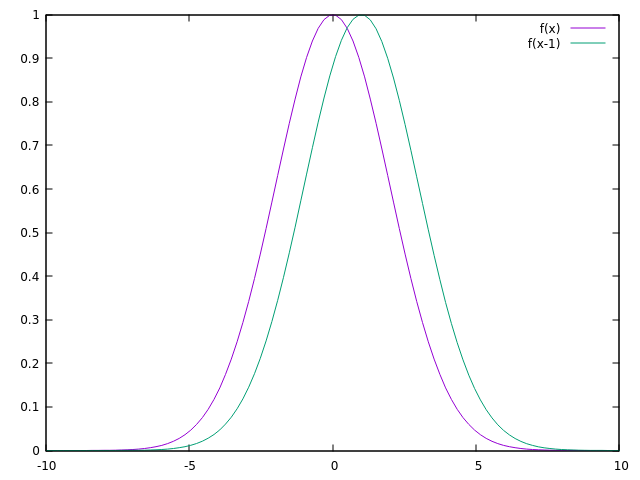
\includegraphics[width=0.5\textwidth]{gnuplot-gaussian.png}
 \caption{Plot of Gaussian functions in \texttt{gnuplot}.}
 \label{fig:gnuplotgaussian}
\end{figure}

\subsection{Using a script file}

While the command line interface is very useful for quick plots, for final figures you will probably need to customize colors, styles, sizes, labels... this can be easily accomplished using a script file, which is simply a text file containing all the commands you want to run. Using your favorite text editor create a file \texttt{gaussian.gp} with the content:

\begin{example}{gnuplot script file `gaussian.gp'}
\begin{minted}[]{gnuplot}
  reset; # cleans the variables and functions
  w = 2.0; # set variable w to store the Gaussian width
  f(x)=exp(-0.5*(x/w)**2); # define a Gaussian function
  set xrange [-10:10]; # set the range of horizontal axes
  set yrange [-0.1:1.1]; # set the range of vertical axes
  set title 'Gaussians'
  set xlabel 'here goes x'
  set ylabel 'here goes f(x)'
  plot f(x) lw 4, f(x-1) lw 2; # plot two functions
\end{minted}
\end{example}

From the \texttt{gnuplot} interface call: \mintinline[escapeinside=||]{gnuplot}{|gnuplot>| load 'gaussian.gp'}. It will open a plot window similar to the previous one, check the differences to understand the new commands on the example.

\subsection{The terminals}

\subsubsection{Example script: epslatex}

\subsection{Using gnuplot with Julia}

\subsection{Most useful commands and examples}

% \section{Another choice: Asymptote}




% ***************************************
\chapter{Other topics \textcolor{red}{(TO DO)}}
\vspace*{-1cm}
\begin{flushright}
\texttt{... and yet another silly quote}
\end{flushright}
\section{Linear algebra}
\section{Root finding}
\section{Linear systems}
\section{Least squares}
% ***************************************


% \chapter{Solution to the proposed problems}
% \section{Problems of Chapter 1}

\subsection*{Problem 1.1: Int64 and Float64}

Float-point numbers (Float64) are approximations of real numbers, while Int64 is for sure an integer. The main different is that if an integer can be expressed with 64 bits, it is exactly expressed. However, if your real number is irrational (which is most often the case) you cannot store it exactly on a computer. Real numbers in computers are always approximated. They are always restricted to numerical errors, specially when we have to deal with comparisons. For instance, after some calculation you end up with two numbers $A$ and $B$. If they are for sure integers (Int64 indeed), you may check if they are equal using a simple command as \texttt{if A == B ...}, however, if they are Float64, the equality could fail due to possible numerical fluctuations at irrelevant decimal cases. So, a comparison should be done as \texttt{if abs(A-B) < abstol ...}, where \texttt{abstol} is a small number (say $10^{-8}$) that specifies your tolerance for the equality.


\subsection*{Problem 1.2: Bhaskara}

\begin{minted}[mathescape]{julia}
# define a function that receives a, b, c, and solve $ax^2 + bx + c = 0$
function bhaskara(a, b, c)
  # calculates $\Delta = b^2 - 4ac$
  delta = b^2 - 4a*c;
  # if $\Delta < 0$, convert it to Complex
  delta = (delta>0.0) ? delta : convert(Complex{Float64}, delta);
  r1 = (-b+sqrt(delta))/(2a); # first root
  r2 = (-b-sqrt(delta))/(2a); # second root
  return (r1, r2); # return roots as a tuple
end

# call the function Bhaskara with parameters a=2, b=-2, c=-12
# as indicated by the tuple above:
# root1 will receive the first root
# root2 will receive the second root
root1, root2 = bhaskara(2.0, -2.0, -12.0);
# print the results on screen
println("The first root is ", root1)
println("The second root is ", root2)

# testing the code for negative $\Delta$
root1, root2 = bhaskara(2.0, -2.0, +12.0);
println("The first root is ", root1)
println("The second root is ", root2)
\end{minted}

\subsection*{Problem 1.3: Scripts}

If you run your script from inside Julia using the \texttt{include} command, you have access to the variables after the code finishes, and you can use \texttt{PyPlot} to plot your data on a plot window. If you run from the BASH command line, you have to save into files, or print on the screen everything you'll need later on. 

\subsection*{Problem 1.5: Conditional evaluations}

\begin{minted}[mathescape,escapeinside=||]{julia}
using PyPlot # start the PyPlot package

# psi receives two parameters: x and a
# you could've set ``a'' globaly as well
psi(x,a) = (abs(x)>a) ? 1.0 : (x/a)^2; # ternary operator (short if)

# using a different letter for the limits just to remind you about the scopes
b = 10.0; 

xvec = linspace(-2b, 2b, 100); # x vector
# calculate psi for each x in xvec and save as a vector f
f = [ psi(x, b) for x=xvec ]; # comprehension

# plot the result
plot(xvec, f);  # $\text{see Fig. \ref{fig:probl1.5}}$
axis([-2b, 2b, 0.0, 1.1]);
\end{minted}

\begin{figure}[ht!]
 \centering
 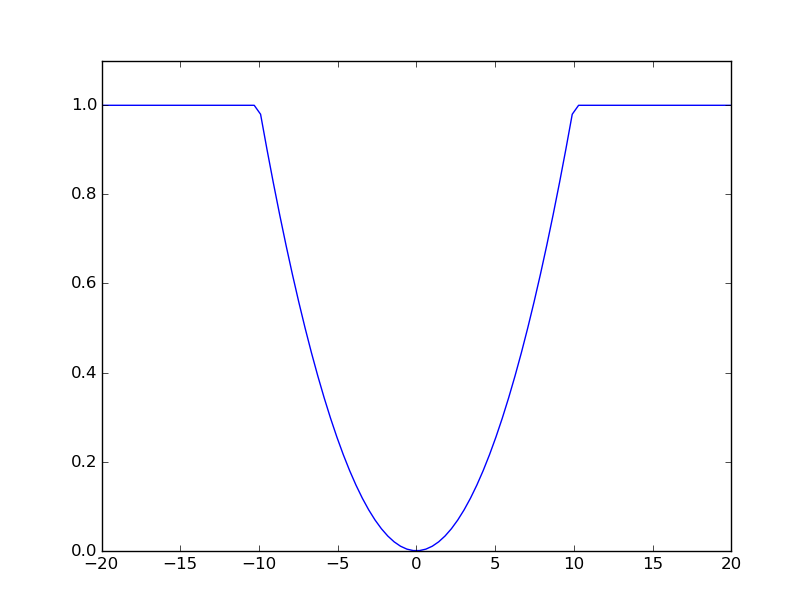
\includegraphics[width=10cm,keepaspectratio=true]{Prob-1-5.png}
 \caption{Output figure of Problem 1.5.}
 \label{fig:probl1.5}
\end{figure}

\subsection*{Problem 1.6: While and For Loops}

\begin{minted}[mathescape]{julia}
# fact receives $n$ and calculates $n!$
function fact(n::Int64)
    res = 1; # initialize the result as 1 since $n! = 1\cdot 2 \cdot 3 \cdot 4 \cdots n$
    i = n; # initialize the counter
    while i > 1 # looping from n to 1
        res = res*i; # since $n! = 1\cdot 2 \cdot 3 \cdot 4 \cdots n$
        i = i-1; # decrease counter
    end # end loop
    return res; # return the result
end

# test the code
fact(4)
\end{minted}


\subsection*{Problem 1.7: Input and Output}

\begin{minted}[mathescape]{julia}
# assuing that the content of bar.dat is
#  1.0   2.0   3.0   4.0   5.0
#  6.0   7.0   8.0   8.0   9.0
# 10.0  11.0  12.3  13.0  14.0
# 15.0  16.0  17.3  18.2  19.0
# 20.1  21.0  22.3  24.0  25.0

# a) read the CSV file
data = readcsv("bar.dat");

# and write using ; separator
writedlm("semicolon.dat", data, ';');

# b) read the ; separated file as String
data = readdlm("semicolon.dat", ';', ASCIIString);

# and write it back as text.dat
writedlm("text.dat", data);
\end{minted}


\subsection*{Problem 1.8:  Random numbers and histograms}

\begin{minted}[mathescape]{julia}
using PyPlot # start the package

list = randn(100000); # sample many random numbers
x, y = hist(list, 100); # calculate the historam with 100 bins

# x has the bin limits
# y has the bin counts
# to plot we need the bin middlepoint:
xav = (x[1:end-1] + x[2:end])/2;

# plot the histogram
plot(xav,  y);

# compare with the PyPlot :hist function
out = plt[:hist](list, 100); # also using 100 bins
x = out[2]; # equivalent to x from hist
y = out[1]; # equivalent to y from hist

# $\text{see output in Fig. \ref{fig:probl1.8}}$
\end{minted}

\begin{figure}[ht!]
 \centering
 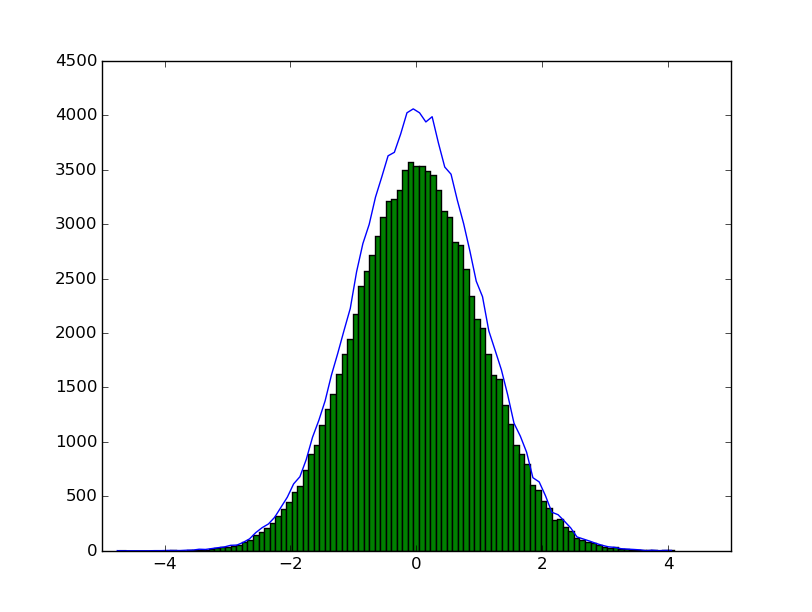
\includegraphics[width=10cm,keepaspectratio=true]{Prob-1-8.png}
 \caption{Output figure of Problem 1.8.}
 \label{fig:probl1.8}
\end{figure}


\subsection*{Problem 1.9: Cross and dot products}

\begin{minted}[mathescape]{julia}
# always use column vectors, since line vectors are seen as matrices
a = [1; 0; 0]; 
b = [0; 1; 0];
c = [5; 5; 1];

v = dot(a, cross(b,c)); # $v = a \cdot (b\times c)$
\end{minted}

\subsection*{Problem 1.10: Calculate $\pi$ using random numbers}

\begin{minted}[mathescape]{julia}
using PyPlot

# initialize vectors to store points
vecin = [0.0 0.0]; # these will be deleted afterwards
vecout = [0.0 0.0]; # these will be deleted afterwards

Pn = 0; # initilize vector to store Pi as a function of n
in=0; # initialize number of in points
out=0; # initialize number of out points
x=1:1000; # range of sampled points

for i=x # loop
    r = rand(2); # sample a point r=(x, y)
    if norm(r) <= 1 # if $|r| < 1$ the point is inside the circle
        in += 1; # increase the in counter
        vecin = [vecin; r[1] r[2]]; # store the point r=(x,y)
    else
        out += 1; # increase the out counter if point is out of the circle
        vecout = [vecout; r[1] r[2]]; # store the out point
    end
    Pn = [Pn; 4*in/(in+out)]; # recalculate pi and store each partial result
end

# the [2:end] below is used to ignore the first data from initialization

subplot(121)
plot(x, Pn[2:end]); # plot partial results as a function of n

subplot(122) # plot stored points
scatter(vecin[2:end,1], vecin[2:end,2], color="blue")
scatter(vecout[2:end,1], vecout[2:end,2], color="red") # see output in $\text{Fig. \ref{fig:probl1.10}}$

# 
\end{minted}


\begin{figure}[ht!]
 \centering
 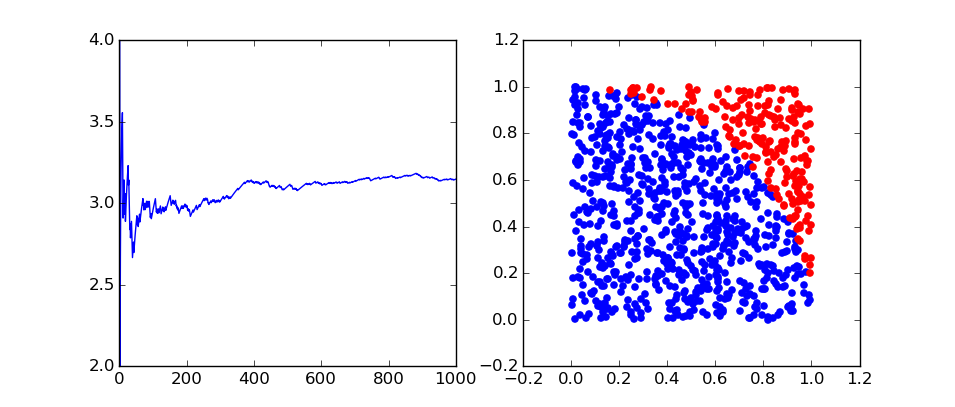
\includegraphics[width=15cm,keepaspectratio=true]{Prob-1-10.png}
 \caption{Output figure of Problem 1.10.}
 \label{fig:probl1.10}
\end{figure}





















% \postextual
\bibliography{biblio}
\end{document}
